% ============================================================
%  EduBoard – Plateforme E-Learning Intelligente avec IA
%  Rapport de Projet de Fin d'Études – ESPITA 2025/2026
%  Auteure : Hayet BERRIRI
% ============================================================
\documentclass[12pt, a4paper, twoside]{report}

% ---- Encodage & langue ----
\usepackage[utf8]{inputenc}
\usepackage[T1]{fontenc}
\usepackage[french]{babel}

% ---- Mise en page ----
\usepackage[top=2.5cm, bottom=2.5cm, left=3cm, right=2.5cm]{geometry}
\usepackage{setspace}
\onehalfspacing
\usepackage{fancyhdr}
\usepackage{emptypage}

% ---- Typographie ----
\usepackage{lmodern}
\usepackage{microtype}

% ---- Graphiques & couleurs ----
\usepackage{graphicx}
\usepackage[dvipsnames,table]{xcolor}
\usepackage{pdfpages}
\graphicspath{{figures/images/}{figures/diagrams/}{figures/pdfs/}}

% ---- Tableaux ----
\usepackage{booktabs}
\usepackage{longtable}
\usepackage{multirow}
\usepackage{array}
\usepackage{tabularx}

% ---- Code source ----
\usepackage{listings}
\usepackage{minted}   % requiert --shell-escape

% ---- Liens & références ----
\usepackage[hidelinks, colorlinks=true,
            linkcolor=espitablue,
            urlcolor=espitablue,
            citecolor=espitablue]{hyperref}
\usepackage{amsmath, amssymb}
% ---- Divers ----
\usepackage{acronym}
\usepackage{pifont}
\usepackage{float}
\usepackage{caption}
\usepackage{subcaption}
\usepackage{enumitem}
\usepackage{amsmath, amssymb}
\usepackage{titlesec}   % personnalisation des titres

% ============================================================
%  COULEURS – extraites du PDF original
% ============================================================
\definecolor{espitablue}{RGB}{31, 78, 151}   % bleu foncé principal
\definecolor{headergray}{RGB}{89, 89, 89}    % gris en-tête (non utilisé ici)

% ============================================================
%  STYLE DES TITRES – bleu, comme dans le PDF
% ============================================================
% Chapitre : "Chapitre N" en petit bleu, titre en grand bleu
\titleformat{\chapter}[display]
  {\normalfont\bfseries\color{espitablue}}
  {\large Chapitre \thechapter}
  {4pt}
  {\Huge}

% Section : bleu gras
\titleformat{\section}
  {\normalfont\large\bfseries\color{espitablue}}
  {\thesection}{1em}{}

% Subsection : bleu gras
\titleformat{\subsection}
  {\normalfont\normalsize\bfseries\color{espitablue}}
  {\thesubsection}{1em}{}

% Subsubsection : bleu normal
\titleformat{\subsubsection}
  {\normalfont\normalsize\bfseries\color{espitablue}}
  {\thesubsubsection}{1em}{}

% ============================================================
%  EN-TÊTES – style exact du PDF original
%  Gauche (pages paires) : EduBoard – Plateforme E-Learning Intelligente  (bleu italique)
%  Droite (pages impaires) :  Hayet BERRIRI  (bleu italique)
%  Ligne de séparation en dessous
% ============================================================
\pagestyle{fancy}
\fancyhf{}

% Pages paires (gauche) : titre du rapport | pages impaires (droite) : auteure
\fancyhead[LE]{\textcolor{espitablue}{\textit{EduBoard -- Plateforme E-Learning Intelligente}}}
\fancyhead[RO]{\textcolor{espitablue}{\textit{Hayet BERRIRI}}}

% Numéro de page centré en pied de page
\fancyfoot[C]{\thepage}

% Ligne d'en-tête en bleu, épaisseur 0.4pt
\renewcommand{\headrule}{%
  {\color{espitablue}\hrule width\headwidth height 0.4pt}}
\renewcommand{\headrulewidth}{0.4pt}

% Ligne de pied de page fine
\renewcommand{\footrulewidth}{0.4pt}
\renewcommand{\footrule}{%
  {\color{espitablue}\hrule width\headwidth height 0.4pt}}

% Style pour les pages de début de chapitre (plain)
\fancypagestyle{plain}{%
  \fancyhf{}%
  \fancyfoot[C]{\thepage}%
  \renewcommand{\headrulewidth}{0pt}%
  \renewcommand{\footrulewidth}{0.4pt}%
  \renewcommand{\footrule}{{\color{espitablue}\hrule width\headwidth height 0.4pt}}%
}

% ============================================================
%  LÉGENDES – petites et centrées
% ============================================================
\captionsetup{font=small, labelfont={bf,color=espitablue}, textfont=it}

% ============================================================
\begin{document}

% ---- Page de garde ----
% ============================================================
%  01_page_garde.tex  –  Page de garde & page jury
% ============================================================
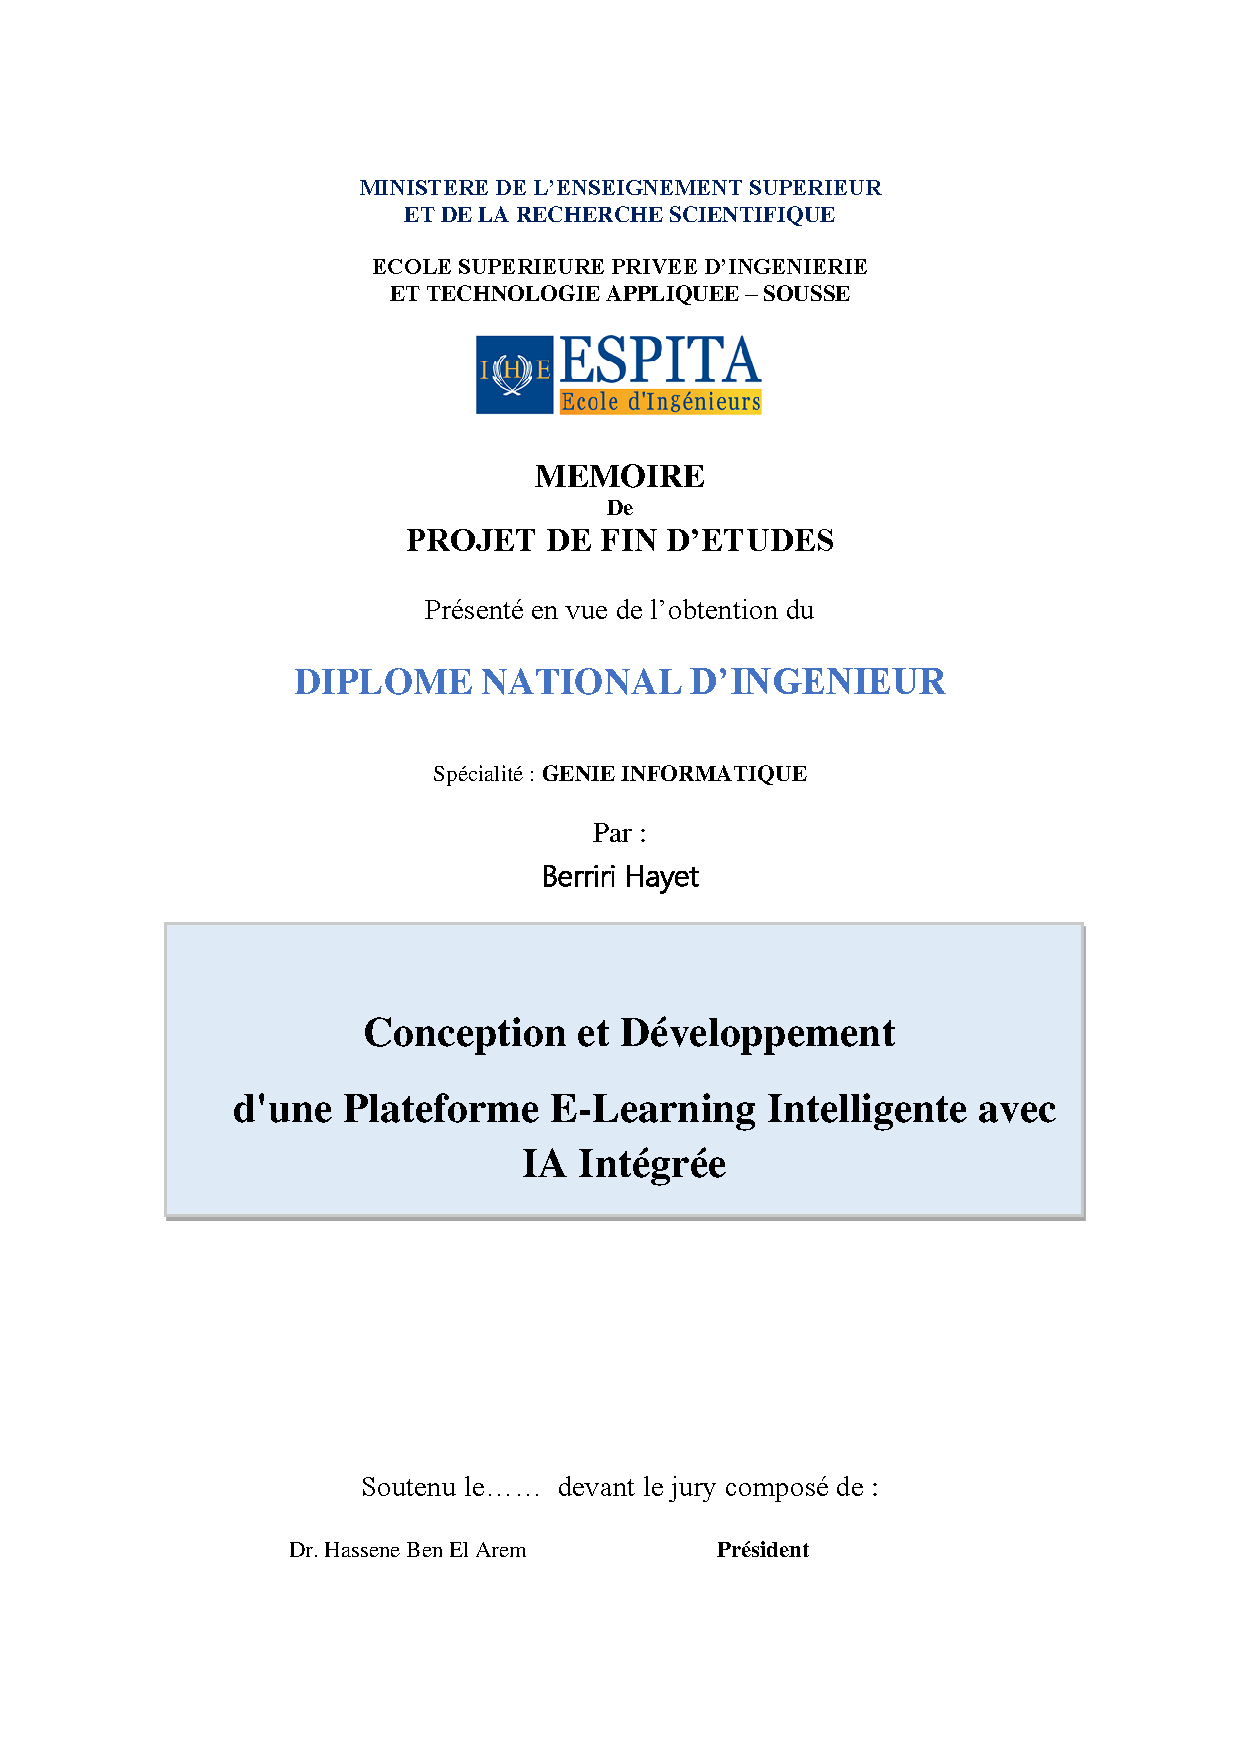
\includepdf[pages=-]{figures/pdfs/page de garde1.pdf}

\clearpage


% ---- Dédicaces ----
% ============================================================
%  02_dedicaces.tex  –  Dédicaces
% ============================================================
\chapter*{Dédicaces}
\addcontentsline{toc}{chapter}{Dédicaces}
\thispagestyle{empty}

\begin{center}
\textit{Du plus profond de mon cœur, je dédie ce travail à toutes les\\
personnes qui me sont chères\ldots}
\end{center}

\vspace{1cm}

\noindent\textbf{À ma précieuse fille Céline,}\\
source inépuisable de motivation, dont le sourire et la présence ont illuminé mes
journées et m'ont donné la force de persévérer.

\vspace{0.8cm}

\noindent\textbf{À mon cher mari Selim,}\\
j'exprime ma profonde reconnaissance pour son soutien indéfectible, sa patience et
ses encouragements constants. Sa présence à mes côtés a été essentielle tout au long
de ce parcours.

\vspace{0.8cm}

\noindent\textbf{À mes chers parents,}\\
ma mère Laila et mon père Taoufik, pour leur amour inconditionnel, leurs sacrifices
et leur confiance. Vous avez été et demeurez une source d'inspiration, de courage et
de force.

\vspace{0.8cm}

\noindent\textbf{À ma belle-famille,}\\
que je considère comme une seconde famille, pour sa bienveillance et son soutien
précieux.

\vspace{0.8cm}

\noindent\textbf{À ma chère amie Maissa,}\\
pour sa présence constante, son écoute et son soutien dans les moments de joie
comme dans les moments de doute.

\vspace{2cm}
\begin{flushright}
\textit{Hayet}
\end{flushright}


% ---- Remerciements ----
% ============================================================
%  03_remerciements.tex  –  Remerciements
% ============================================================
\chapter*{Remerciements}
\addcontentsline{toc}{chapter}{Remerciements}
\thispagestyle{empty}

En premier lieu, je remercie Dieu le tout-puissant de m'avoir accordé la volonté,
la patience et la santé nécessaires pour accomplir ce travail.
\vspace{0.5cm}


Je tiens à exprimer ma profonde reconnaissance à mon encadrant académique,
\textbf{Anouar Bouazza}, pour son encadrement bienveillant, ses conseils pertinents
et le temps précieux qu'il m'a consacré tout au long de ce projet.
\vspace{0.5cm}


Mes sincères remerciements vont à mon encadrant professionnel \textbf{Wael Boukadida}
au sein de Whitecape Technologies, pour son accueil chaleureux, sa disponibilité permanente et son accompagnement expert qui ont permis de mener ce projet à bien dans les meilleures conditions.
\vspace{0.5cm}


Je remercie l'ensemble de l'équipe de Whitecape Technologies, société franco-tunisienne
reconnue pour son expertise nearshore depuis 2008, pour leur professionnalisme, leur
esprit d'équipe et leur soutien technique tout au long de mon stage.
\vspace{0.5cm}

Je tiens également à remercier les membres du jury qui ont bien voulu accepter
d'évaluer ce travail et lui accorder de l'intérêt.
\vspace{0.5cm}

Mes remerciements vont enfin à tous mes enseignants qui ont contribué à ma
formation et à tous ceux qui, de près ou de loin, ont participé à la réalisation de
ce projet.


% ---- Front matter ----
\pagenumbering{roman}
\setcounter{page}{1}

\tableofcontents
\clearpage

\listoffigures
\clearpage

\listoftables
\clearpage

% ---- Liste des abréviations ----
% ============================================================
%  00_acronymes_def.tex  –  Définition des acronymes (package acronym)
% ============================================================
\chapter*{Liste des Abréviations}
\addcontentsline{toc}{chapter}{Liste des Abréviations}

\begin{acronym}[XXXXXX]
%  \acro{API}  {Application Programming Interface}
  \acro{ASP}  {Active Server Pages}
  \acro{BDD}  {Base De Données}
  \acro{BLOB} {Binary Large Object}
  \acro{CORS} {Cross-Origin Resource Sharing}
  \acro{CRUD} {Create, Read, Update, Delete}
  \acro{EF}   {Entity Framework}
  \acro{IA}   {Intelligence Artificielle}
  \acro{JWT}  {JSON Web Token}
  \acro{LLM}  {Large Language Model}
  \acro{MVC}  {Model-View-Controller}
  \acro{ORM}  {Object-Relational Mapping}
  \acro{PFE}  {Projet de Fin d'Études}
  \acro{REST} {Representational State Transfer}
  \acro{SPA}  {Single Page Application}
  \acro{SQL}  {Structured Query Language}
  \acro{SaaS} {Software as a Service}
  \acro{SSL}  {Secure Sockets Layer}
  \acro{TLS}  {Transport Layer Security}
  \acro{UI}   {User Interface}
  \acro{UML}  {Unified Modeling Language}
  \acro{UX}   {User Experience}
\end{acronym}

\clearpage

% ---- Corps du rapport ----
\pagenumbering{arabic}
\setcounter{page}{1}

% ============================================================
%  05_introduction_generale.tex  –  Introduction Générale
% ============================================================
\chapter*{Introduction Générale}
\addcontentsline{toc}{chapter}{Introduction Générale}
\markboth{Introduction Générale}{Introduction Générale}

La transformation numérique a profondément modifié les pratiques d'apprentissage,
aussi bien dans les établissements d'enseignement que dans les entreprises. Dans un
contexte marqué par la formation à distance, la montée en puissance de la formation
continue et l'évolution rapide des compétences numériques, les plateformes e-learning
sont devenues des outils essentiels pour diffuser, suivre et évaluer les apprentissages.
\vspace{1cm}
\medskip


Toutefois, de nombreuses solutions existantes restent limitées par une faible personnalisation
des parcours, des évaluations essentiellement quantitatives et une assistance pédagogique
insuffisante. L'émergence de l'intelligence artificielle générative, notamment des grands
modèles de langage, offre de nouvelles perspectives pour accompagner les apprenants,
automatiser certaines tâches pédagogiques et proposer des recommandations adaptées
aux besoins réels des étudiants.
\vspace{1cm}

\medskip

C'est dans ce cadre que s'inscrit le présent projet de fin d'études, réalisé au sein de
Whitecape Technologies. Il porte sur la conception et le développement d'\textbf{EduBoard},
une plateforme e-learning intelligente visant à combiner gestion pédagogique, suivi
de progression, évaluation assistée par \ac{IA}, recommandation personnalisée, chatbot
pédagogique et génération automatique de certificats.
\vspace{1cm}

\medskip

Ce rapport est organisé en quatre chapitres principaux, encadrés par une introduction
et une conclusion générales~:
\vspace{0.5cm}

\begin{itemize}
  \item \textbf{Chapitre~1} présente le contexte général du projet~: l'organisme
        d'accueil, la problématique, l'étude de l'existant, la solution proposée et la
        méthodologie de travail.
  \item \textbf{Chapitre~2} expose la spécification détaillée des besoins fonctionnels
        et non fonctionnels, avec les diagrammes \ac{UML} de cas d'utilisation et les
        scénarios principaux.
  \item \textbf{Chapitre~3} détaille la conception globale de la solution~: architecture,
        modèle de données, diagrammes d'activité, de séquence, de classes et de
        déploiement.
  \item \textbf{Chapitre~4} présente la réalisation concrète, les interfaces développées
        et les tests de validation effectués.
\end{itemize}

% ============================================================
%  06_chapitre1_presentation.tex  –  Chapitre 1 : Contexte Général
% ============================================================
\chapter{Contexte Général du Projet}

\section*{Introduction}
\addcontentsline{toc}{section}{Introduction}

Ce premier chapitre pose les bases de notre travail. Il présente l'organisation hôte,
le problème auquel notre solution répond, l'étude de la situation existante, la solution
adoptée et la méthodologie de travail choisie.

% ------------------------------------------------------------
\section{Cadre du Projet}

\subsection{Présentation de l'organisme d'accueil : Whitecape Technologies}

Whitecape Technologies est une entreprise franco-tunisienne spécialisée dans le
développement de solutions informatiques sur mesure. Située à Sousse, en Tunisie,
l'entreprise possède une vaste expérience en gestion de projets tant localement qu'en
modèle nearshore. Whitecape Technologies se distingue par son expertise dans la
création de solutions innovantes adaptées aux besoins spécifiques de chaque client,
en s'appuyant sur des équipes pluridisciplinaires et hautement qualifiées.

\begin{figure}[H]
  \centering
  
\includegraphics[width=0.35\textwidth]{whitecape_technologies_logo.jpg}
  \caption{Logo de Whitecape Technologies}
  \label{fig:logo_whitecape}
\end{figure}

\subsection{Objectif et Contexte}

Fondée en 2007, Whitecape Technologies vise à devenir un leader dans le secteur
des technologies de l'information en Tunisie et au-delà. L'entreprise se concentre
sur la fourniture de solutions technologiques avancées pour aider les entreprises à
optimiser leurs opérations, améliorer leur productivité et atteindre leurs objectifs
stratégiques.

\subsection{Services et Solutions}

\paragraph{Développement et ingénierie}
\begin{itemize}
  \item Développement d'applications web dynamiques et interactives.
  \item Développement d'applications mobiles iOS et Android.
  \item Solutions sur mesure et DevOps / automatisation (\ac{CI}/\ac{CD}).
\end{itemize}

\paragraph{Consultation en technologie}
Audit, évaluation et définition de la feuille de route technologique.

\paragraph{Intégration des systèmes}
Intégration ERP et CRM, support technique, maintenance préventive et corrective.

\paragraph{Services d'Assurance Qualité}
Tests manuels et automatisés, frameworks d'automatisation, audits qualité.

\medskip
\noindent\textbf{Fiche technique :}
\begin{itemize}
  \item \textbf{Entreprise :} Whitecape Technologies
  \item \textbf{Email :} \href{mailto:info@whitecapetech.com}{info@whitecapetech.com}
  \item \textbf{Téléphone :} +216 31 20 88 88 – +33 5 32 10 80 56
  \item \textbf{Adresse :} Avenue de la République, Akouda 4022, Sousse – Tunisie
  \item \textbf{Site web :} \url{https://www.whitecapetech.com}
\end{itemize}

\subsection{Problématique}

Le marché de la formation en ligne connaît une croissance exponentielle. Cependant,
les solutions existantes présentent des lacunes majeures~:

\begin{itemize}
  \item \textbf{Absence de personnalisation} des parcours selon le niveau et le rythme
        de chaque apprenant.
  \item \textbf{Évaluations statiques} sans feedback pédagogique contextuel.
  \item \textbf{Absence d'assistance 24h/24} pour accompagner l'étudiant.
  \item \textbf{Taux d'abandon élevé} dû au manque de motivation.
  \item \textbf{Gestion administrative lourde} pour enseignants et administrateurs.
\end{itemize}

\medskip
La question centrale est donc~:

\begin{quote}
\textit{Comment concevoir une plateforme e-learning moderne, scalable et intelligente,
qui exploite l'\ac{IA} générative pour personnaliser l'expérience de chaque apprenant
tout en simplifiant la gestion pour les enseignants et administrateurs~?}
\end{quote}

\subsection{Étude de l'existant}

\begin{table}[H]
  \centering
  \caption{Analyse comparative des plateformes e-learning existantes}
  \label{tab:existant}
  \begin{tabularx}{\textwidth}{lXXc}
    \toprule
    \textbf{Plateforme} & \textbf{Points forts} & \textbf{Limitations} & \textbf{\ac{IA}~?} \\
    \midrule
    Moodle      & Open source, flexible, large communauté & Interface vieillissante, installation complexe & Non \\
    \midrule
    Udemy       & Large catalogue (200k+ cours), mobile  & Pas de personnalisation du parcours & Partiel \\
    \midrule
    Coursera    & Certifications reconnues, partenariats universités & Coûteux, peu adapté PME tunisiennes & Partiel \\
    \midrule
    Google Classroom & Intégration Google, simplicité & Très limité, pas de marketplace & Non \\
    \midrule
    \textbf{EduBoard} & IA complète, multi-rôles, chapitres verrouillés, certificats auto & Solution en développement & \textbf{Oui (complet)} \\
    \bottomrule
  \end{tabularx}
\end{table}

\subsection{Solution proposée : EduBoard}

EduBoard est une plateforme e-learning intelligente et complète, développée avec des
technologies modernes. Elle répond à l'ensemble des lacunes identifiées~:

\begin{enumerate}
  \item Gestion multi-rôles avec tableau de bord dédié (Admin, Enseignant, Étudiant).
  \item Cours structurés en chapitres et leçons (article, PDF).
  \item Chapitres verrouillés séquentiellement : accès au chapitre $N$ conditionné
        par la complétion du chapitre $N-1$.
  \item Quiz adaptatifs avec feedback \ac{IA} généré par Claude (Anthropic).
  \item Chatbot pédagogique 7j/7 propulsé par l'API Groq.
  \item Moteur de recommandation basé sur le comportement et la progression.
  \item Génération automatique de certificats PDF via QuestPDF avec QR code.
  \item Système de paiement Flouci pour les cours payants.
\end{enumerate}

% ------------------------------------------------------------
\section{Méthodologie de Travail : SCRUM}

\subsection{Présentation du Framework SCRUM}

\noindent Conformément aux pratiques de gestion de projet adoptées par \textbf{Whitecape Technologies}, le projet EduBoard a été conduit selon une démarche agile inspirée du framework \textbf{SCRUM}. Ce choix se justifie par la nature intrinsèquement évolutive des besoins d'une plateforme e-learning, la nécessité de produire des livrables testables à chaque itération et l'importance d'une communication régulière entre les parties prenantes.

\vspace{0.5cm}

\noindent SCRUM est un cadre de travail agile léger mais puissant, issu de la métaphore du rugby (la mêlée, ou \textit{scrum} en anglais). Il repose sur trois piliers fondamentaux : la \textbf{transparence} (tous les aspects du processus sont visibles par tous), l'\textbf{inspection} (les artefacts et la progression sont régulièrement examinés) et l'\textbf{adaptation} (le plan est ajusté en fonction des résultats des inspections).

\vspace{0.5cm}

\noindent Les éléments constitutifs de SCRUM se déclinent en trois catégories :

\textbf{Rôles :}
\begin{itemize}
  \item \textbf{Product Owner :} Représente les intérêts des parties prenantes, gère et priorise le Product Backlog. Dans notre contexte : l'encadrant professionnel Wael Boukadida.
  \item \textbf{Scrum Master :} Garant de l'application du framework, facilitateur et protecteur de l'équipe. Rôle assumé par l'auteure.
  \item \textbf{Équipe de Développement :} Auto-organisée et pluridisciplinaire. Composée de l'auteure pour le développement full-stack.
\end{itemize}

\textbf{Artefacts :}
\begin{itemize}
  \item \textbf{Product Backlog :} Liste priorisée de toutes les fonctionnalités souhaitées pour le produit final.
  \item \textbf{Sprint Backlog :} Sous-ensemble du Product Backlog sélectionné pour le sprint en cours.
  \item \textbf{Incrément :} Somme de toutes les user stories complétées, constituant une version potentiellement livrable du produit.
\end{itemize}

\textbf{Cérémonies :}
\begin{itemize}
  \item \textbf{Sprint Planning :} Réunion de planification du sprint (objectifs, user stories sélectionnées, estimations).
  \item \textbf{Daily Scrum :} Point quotidien de 15 minutes (avancement, blocages, plan du jour).
  \item \textbf{Sprint Review :} Démonstration et validation des fonctionnalités développées.
  \item \textbf{Sprint Retrospective :} Analyse du processus pour améliorer la productivité et la qualité.
  \vspace{0.7cm}
\end{itemize}

\begin{figure}[H]
    
  \centering
  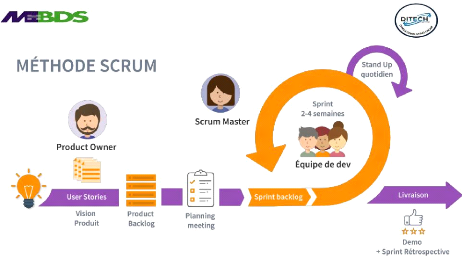
\includegraphics[width=0.85\textwidth]
  {scrum.png}
  \caption{Cycle de vie du framework SCRUM}
  \label{fig:scrum}
\end{figure}


\section*{Conclusion}
\addcontentsline{toc}{section}{Conclusion}

Ce chapitre a posé le cadre du projet~: présentation de l'organisme d'accueil,
analyse de la problématique et des solutions existantes, définition de la solution
EduBoard et planification SCRUM. Le chapitre suivant formalise les besoins fonctionnels
et non fonctionnels de la plateforme.

% ============================================================
%  07_chapitre2_specifications.tex  –  Chapitre 2 : Spécification des Besoins
% ============================================================
\chapter{Spécification des Besoins}

\section*{Introduction}
\addcontentsline{toc}{section}{Introduction}

Ce chapitre présente l'analyse et la modélisation des exigences pour la plateforme
EduBoard. Nous identifions les acteurs, leurs rôles, les exigences fonctionnelles et
non fonctionnelles, puis nous les formalisons à travers des diagrammes \ac{UML}.

% ------------------------------------------------------------
\section{Identification des Acteurs}

La plateforme EduBoard implique trois acteurs humains principaux et un acteur
applicatif~:

\begin{table}[H]
  \centering
  \caption{Description des acteurs de la plateforme EduBoard}
  \label{tab:acteurs}
  \begin{tabularx}{\textwidth}{|l|X|l|}
    \hline
    \textbf{Acteur} & \textbf{Rôle} & \textbf{Accès principal} \\
    \hline
    Administrateur & Supervise la plateforme, gère les utilisateurs et les contenus & \texttt{/dashboard} \\
    \hline
    Enseignant     & Crée et gère les cours, modules, leçons et quiz               & \texttt{/teacher-dashboard} \\
    \hline
    Étudiant       & Consulte, achète les cours, passe les quiz, obtient des certificats & \texttt{/student-dashboard} \\
    \hline
    Système \ac{IA}     & Génère feedback quiz, recommandations, répond au chatbot       & API interne \\
    \hline
  \end{tabularx}
\end{table}

% ------------------------------------------------------------
\section{Diagrammes de Cas d'Utilisation}

\subsection{Diagramme de Cas d'Utilisation Global}

\begin{figure}[H]
  \centering
  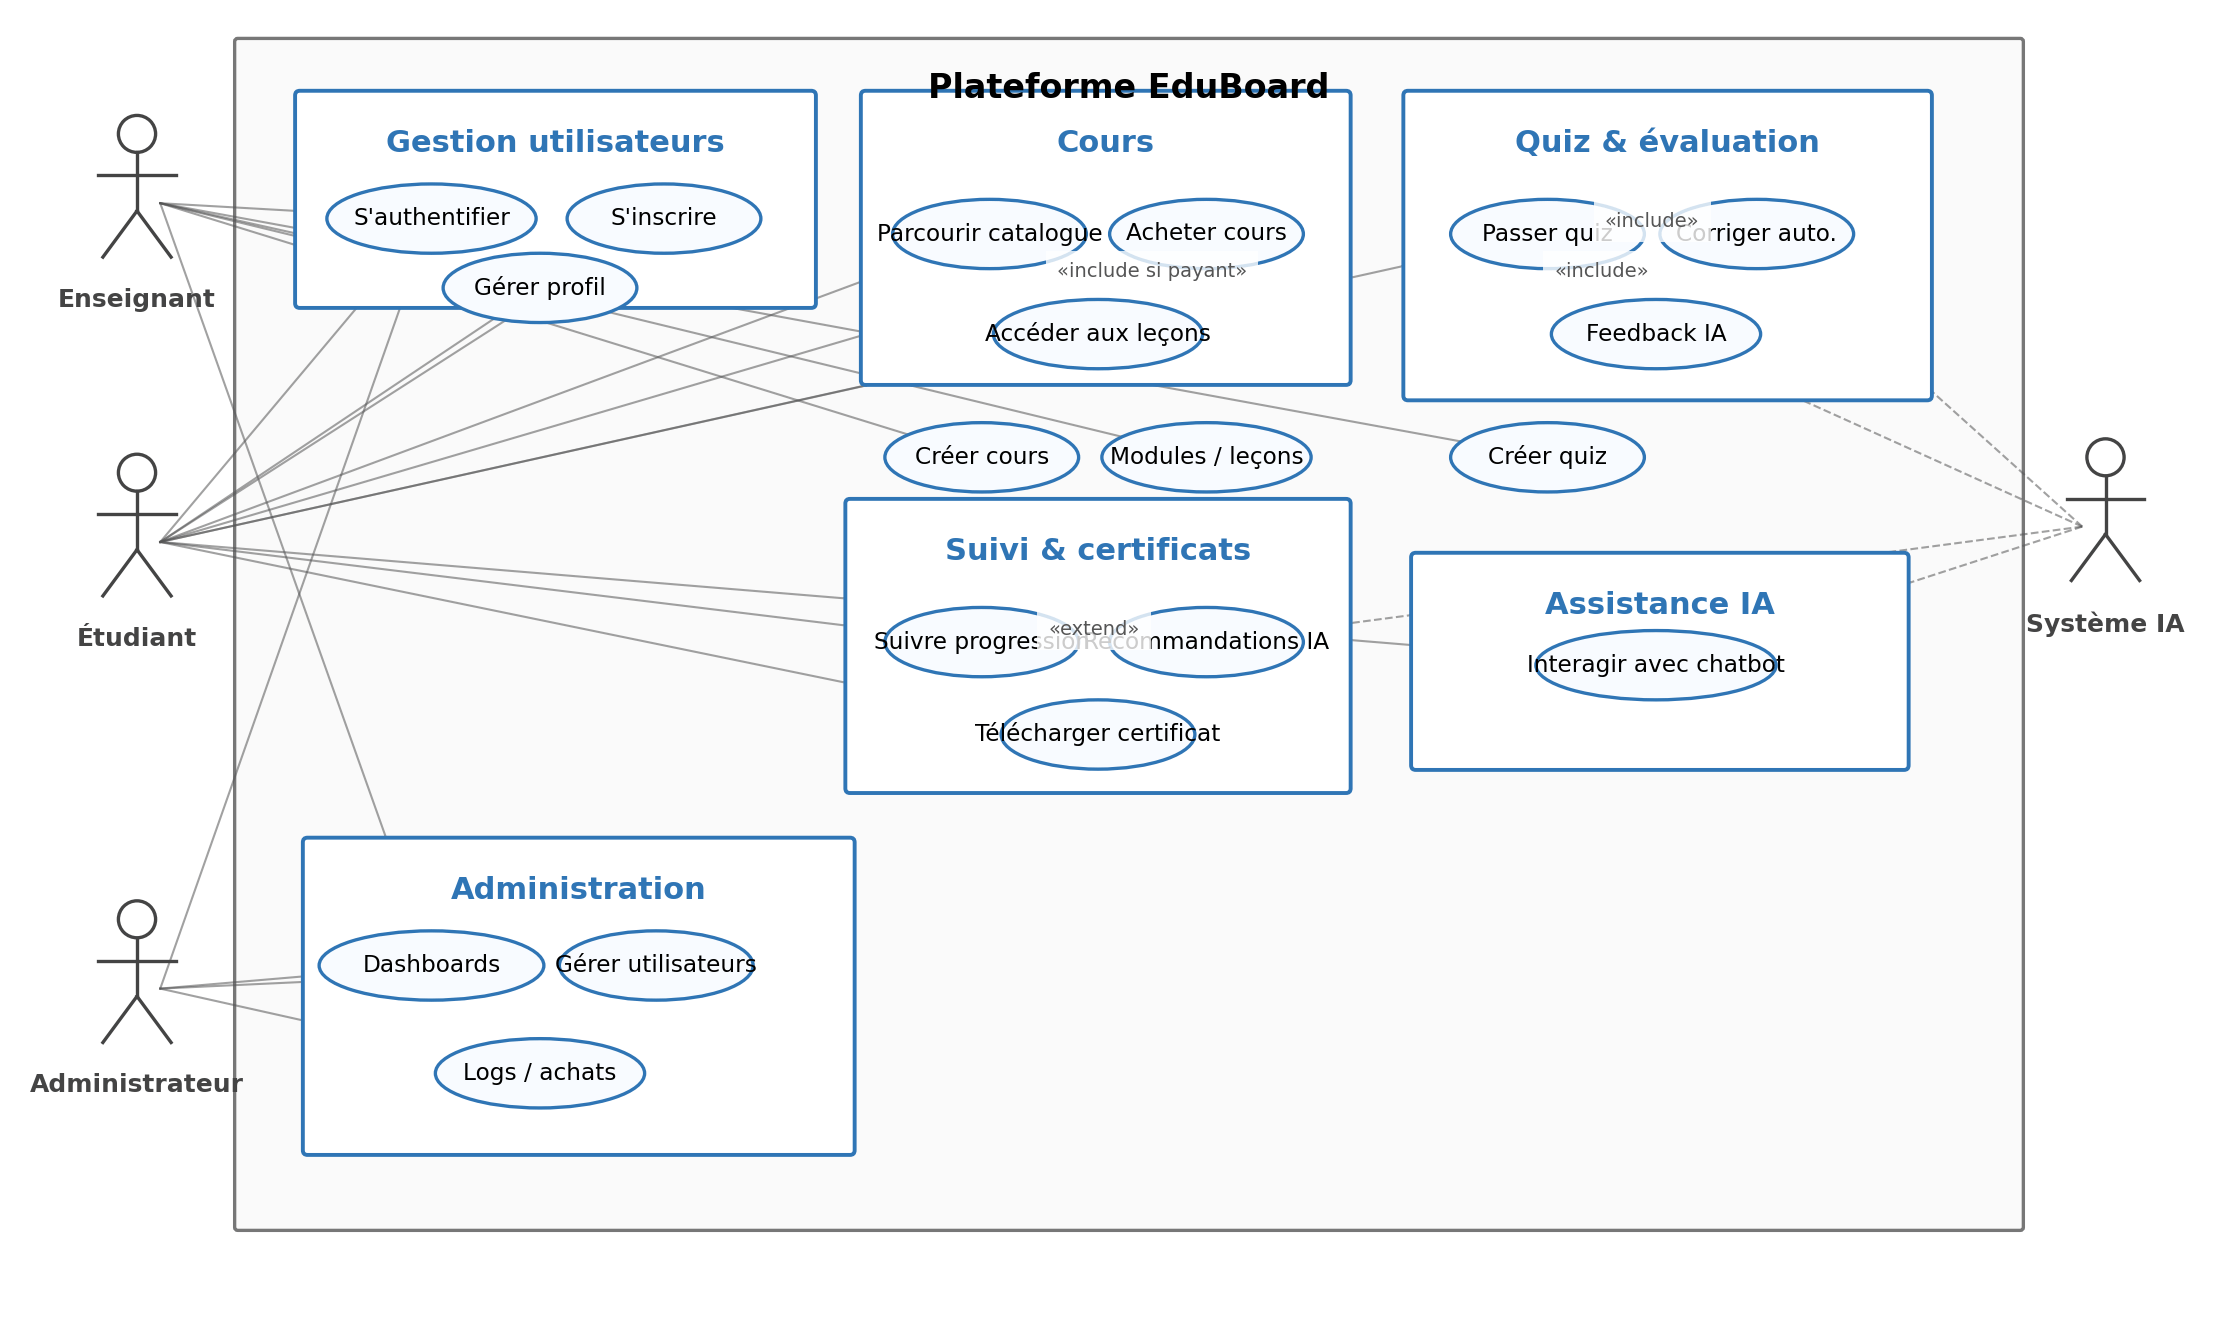
\includegraphics[width=\textwidth]
  {cas_d_utilisation_sprint_1_et_2.png}
  \caption{Diagramme de cas d'utilisation global – Plateforme EduBoard}
  \label{fig:uc_global}
\end{figure}

\noindent  Ce diagramme offre une vue panoramique de l’ensemble des fonctionnalités proposées par la plateforme \textbf{EduBoard} ainsi que de leur répartition entre les différents acteurs du système. Il constitue le document de référence fonctionnel du projet en synthétisant tout le périmètre applicatif au sein d’un schéma unique.

\medskip

\noindent  Son objectif est d’identifier de manière exhaustive les cas d’utilisation du système, les acteurs qui y sont associés ainsi que les relations de dépendance de type \textit{include} et \textit{extend}, afin de garantir une couverture fonctionnelle complète et de faciliter la validation des besoins avec l’ensemble des parties prenantes.

\medskip

\noindent Le diagramme met en évidence quatre acteurs principaux : l’Administrateur, l’Enseignant, l’Étudiant et le Système IA. Les fonctionnalités sont organisées en cinq packages fonctionnels : Authentification, Gestion des cours, Quiz \& Évaluation, Suivi \& Progression et Administration. Il représente également l’héritage entre acteurs, où les trois rôles humains partagent des fonctionnalités communes telles que l’authentification et la gestion du profil. Les relations \textit{include} permettent de modéliser les comportements obligatoirement inclus dans d’autres cas d’utilisation, comme le fait que « Passer un quiz » nécessite préalablement de « S’authentifier ». Les relations \textit{extend} décrivent quant à elles des comportements optionnels venant enrichir un cas d’utilisation principal, à l’image de la génération d’un certificat après la complétion d’un cours.




\medskip

\noindent  Ce diagramme justifie l'architecture multi-rôles de la plateforme et fournit une vision globale des interactions entre les utilisateurs et les différents modules fonctionnels du système.

\subsection{Diagramme de Cas d'Utilisation – Étudiant}

\begin{figure}[H]
  \centering
  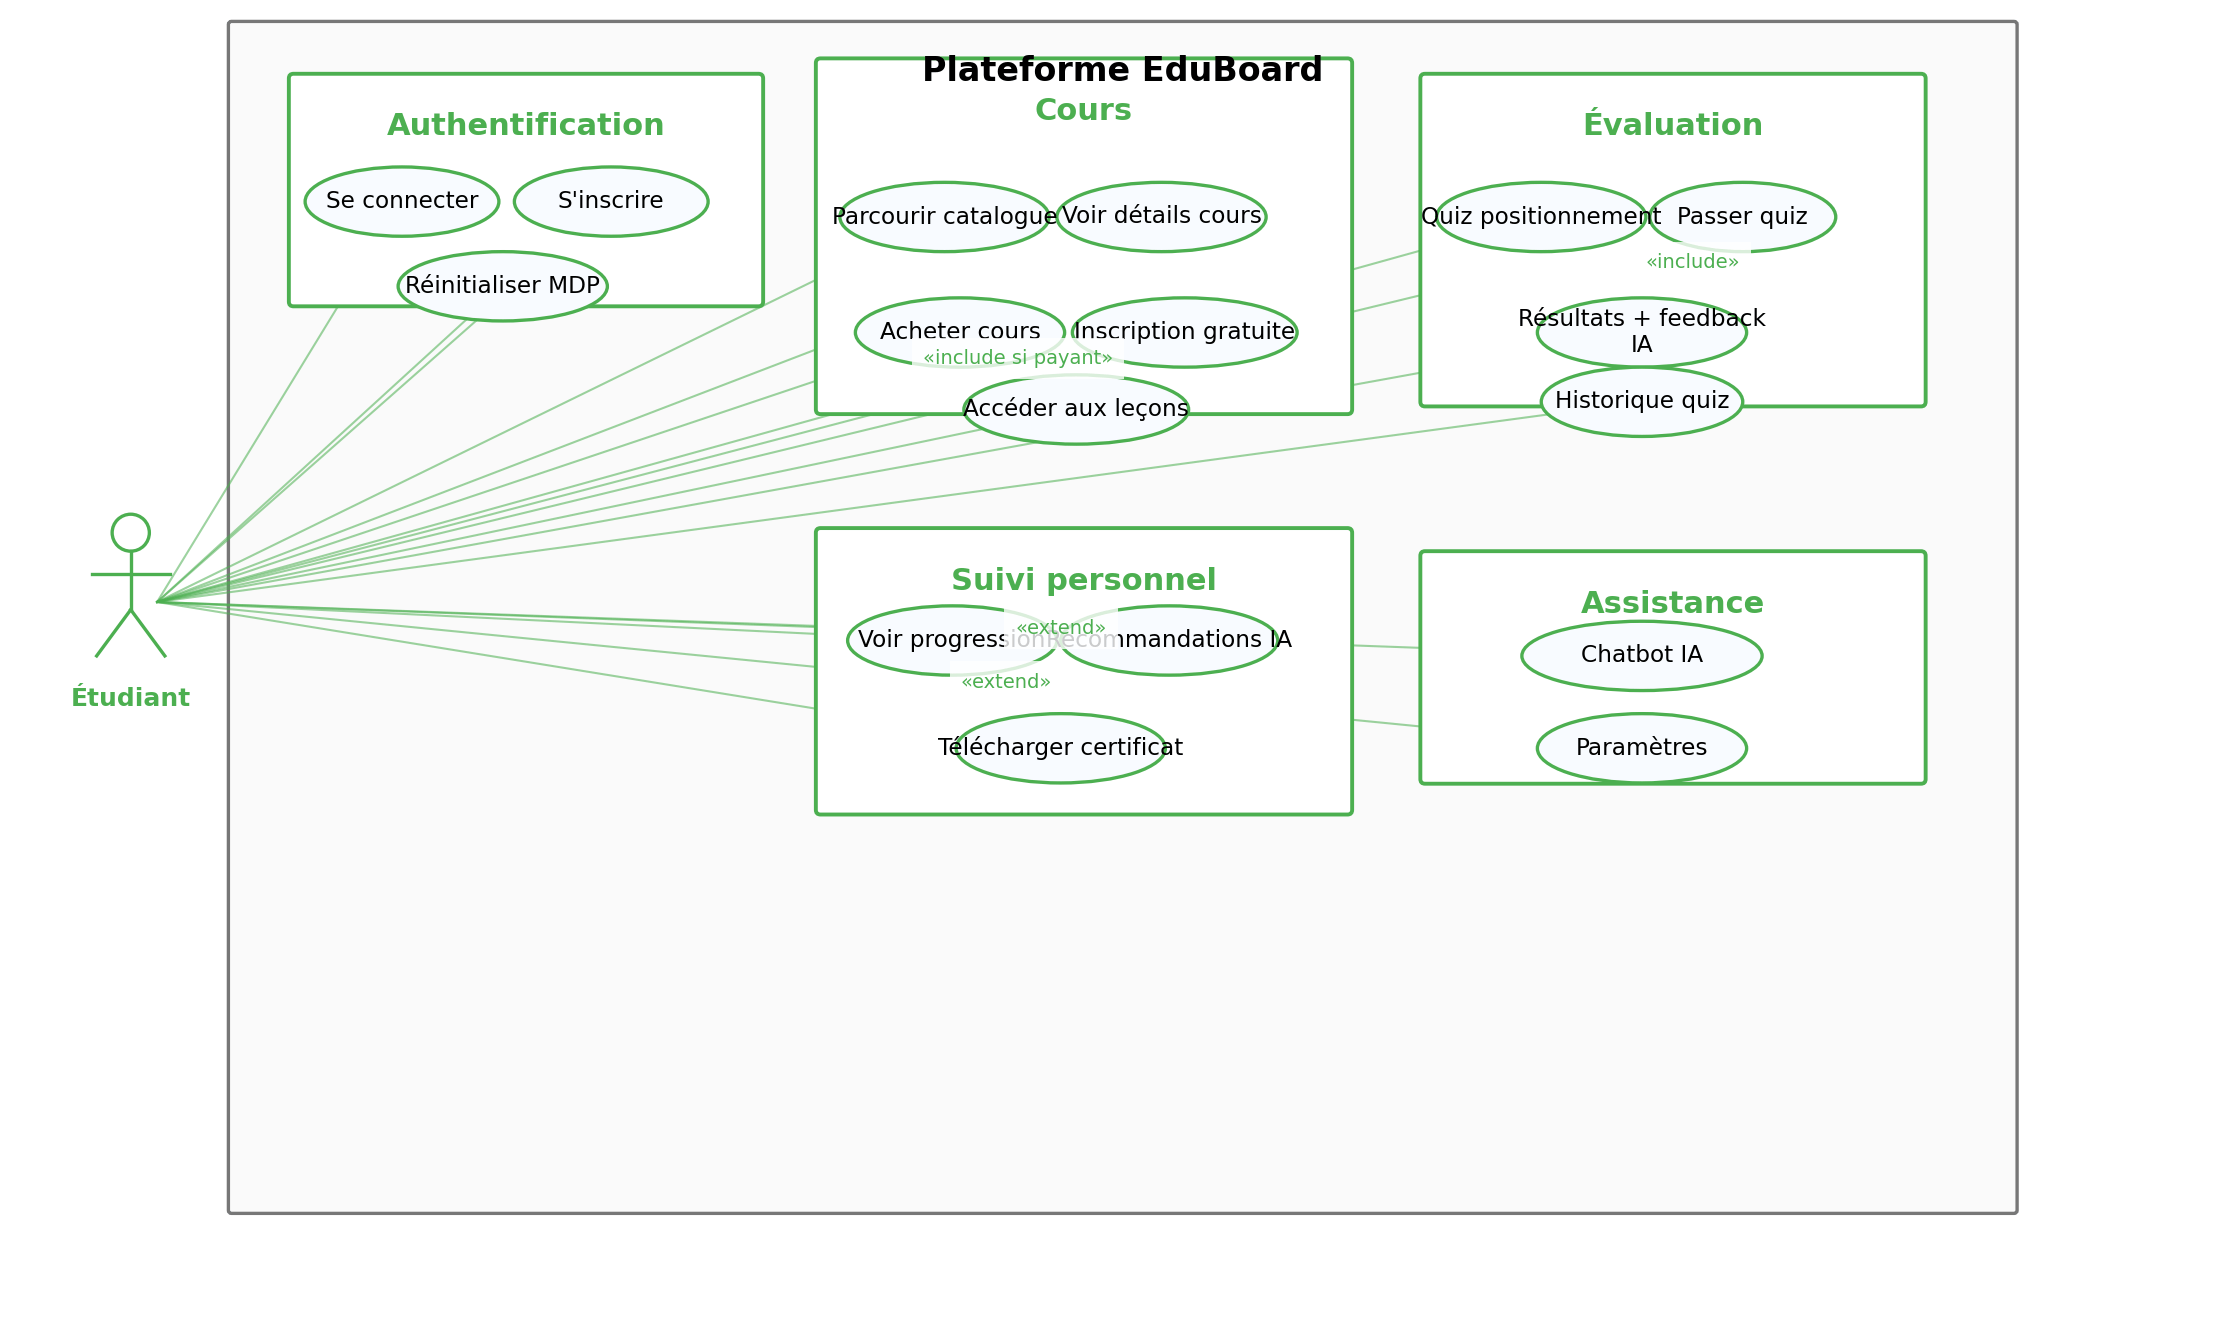
\includegraphics[width=\textwidth]{DIAGRAMME_DE_CAS_D_UTILISATION_-_ETUDIANT.png}
  \caption{Diagramme de cas d'utilisation – Espace Étudiant}
  \label{fig:uc_etudiant}
\end{figure}
\noindent Ce diagramme de cas d'utilisation détaille le périmètre fonctionnel associé à l'acteur \textbf{Étudiant}, principal bénéficiaire de la plateforme \textbf{EduBoard}. Il représente l'ensemble du parcours d'apprentissage, depuis la découverte et l'acquisition des cours jusqu'à leur validation et l'obtention d'un certificat de réussite.

\medskip

\noindent  L'objectif de ce diagramme est de spécifier avec précision les actions accessibles à l'étudiant au sein de son espace dédié (\textit{/student-dashboard}), afin de servir de référence pour le développement des fonctionnalités frontend et backend qui lui sont destinées.

\medskip

\noindent  L'étudiant peut parcourir le catalogue des cours et consulter leurs détails, acheter un cours payant via la solution de paiement \textit{Flouci}, suivre les leçons sous différents formats (vidéos, articles et documents PDF), passer les quiz associés aux chapitres et recevoir un feedback personnalisé généré par l'intelligence artificielle. Il dispose également d'outils lui permettant de consulter sa progression globale ainsi que sa progression par cours, d'accéder à des recommandations personnalisées adaptées à son parcours, de télécharger un certificat au format PDF après la complétion d'un cours et d'interagir avec le chatbot pédagogique basé sur l'intelligence artificielle (\textit{ChatbotWidget}) pour obtenir une assistance en temps réel.

\medskip

\noindent  Une caractéristique essentielle de la plateforme EduBoard réside dans le verrouillage séquentiel des chapitres. L'accès à un chapitre donné est conditionné par la complétion du chapitre précédent ainsi que par la réussite du quiz correspondant. Cette contrainte, modélisée dans le diagramme à travers une relation \textit{extend}, garantit une progression pédagogique structurée et favorise l'acquisition progressive des connaissances.

\subsection{Diagramme de Cas d'Utilisation – Enseignant}

\begin{figure}[H]
  \centering
  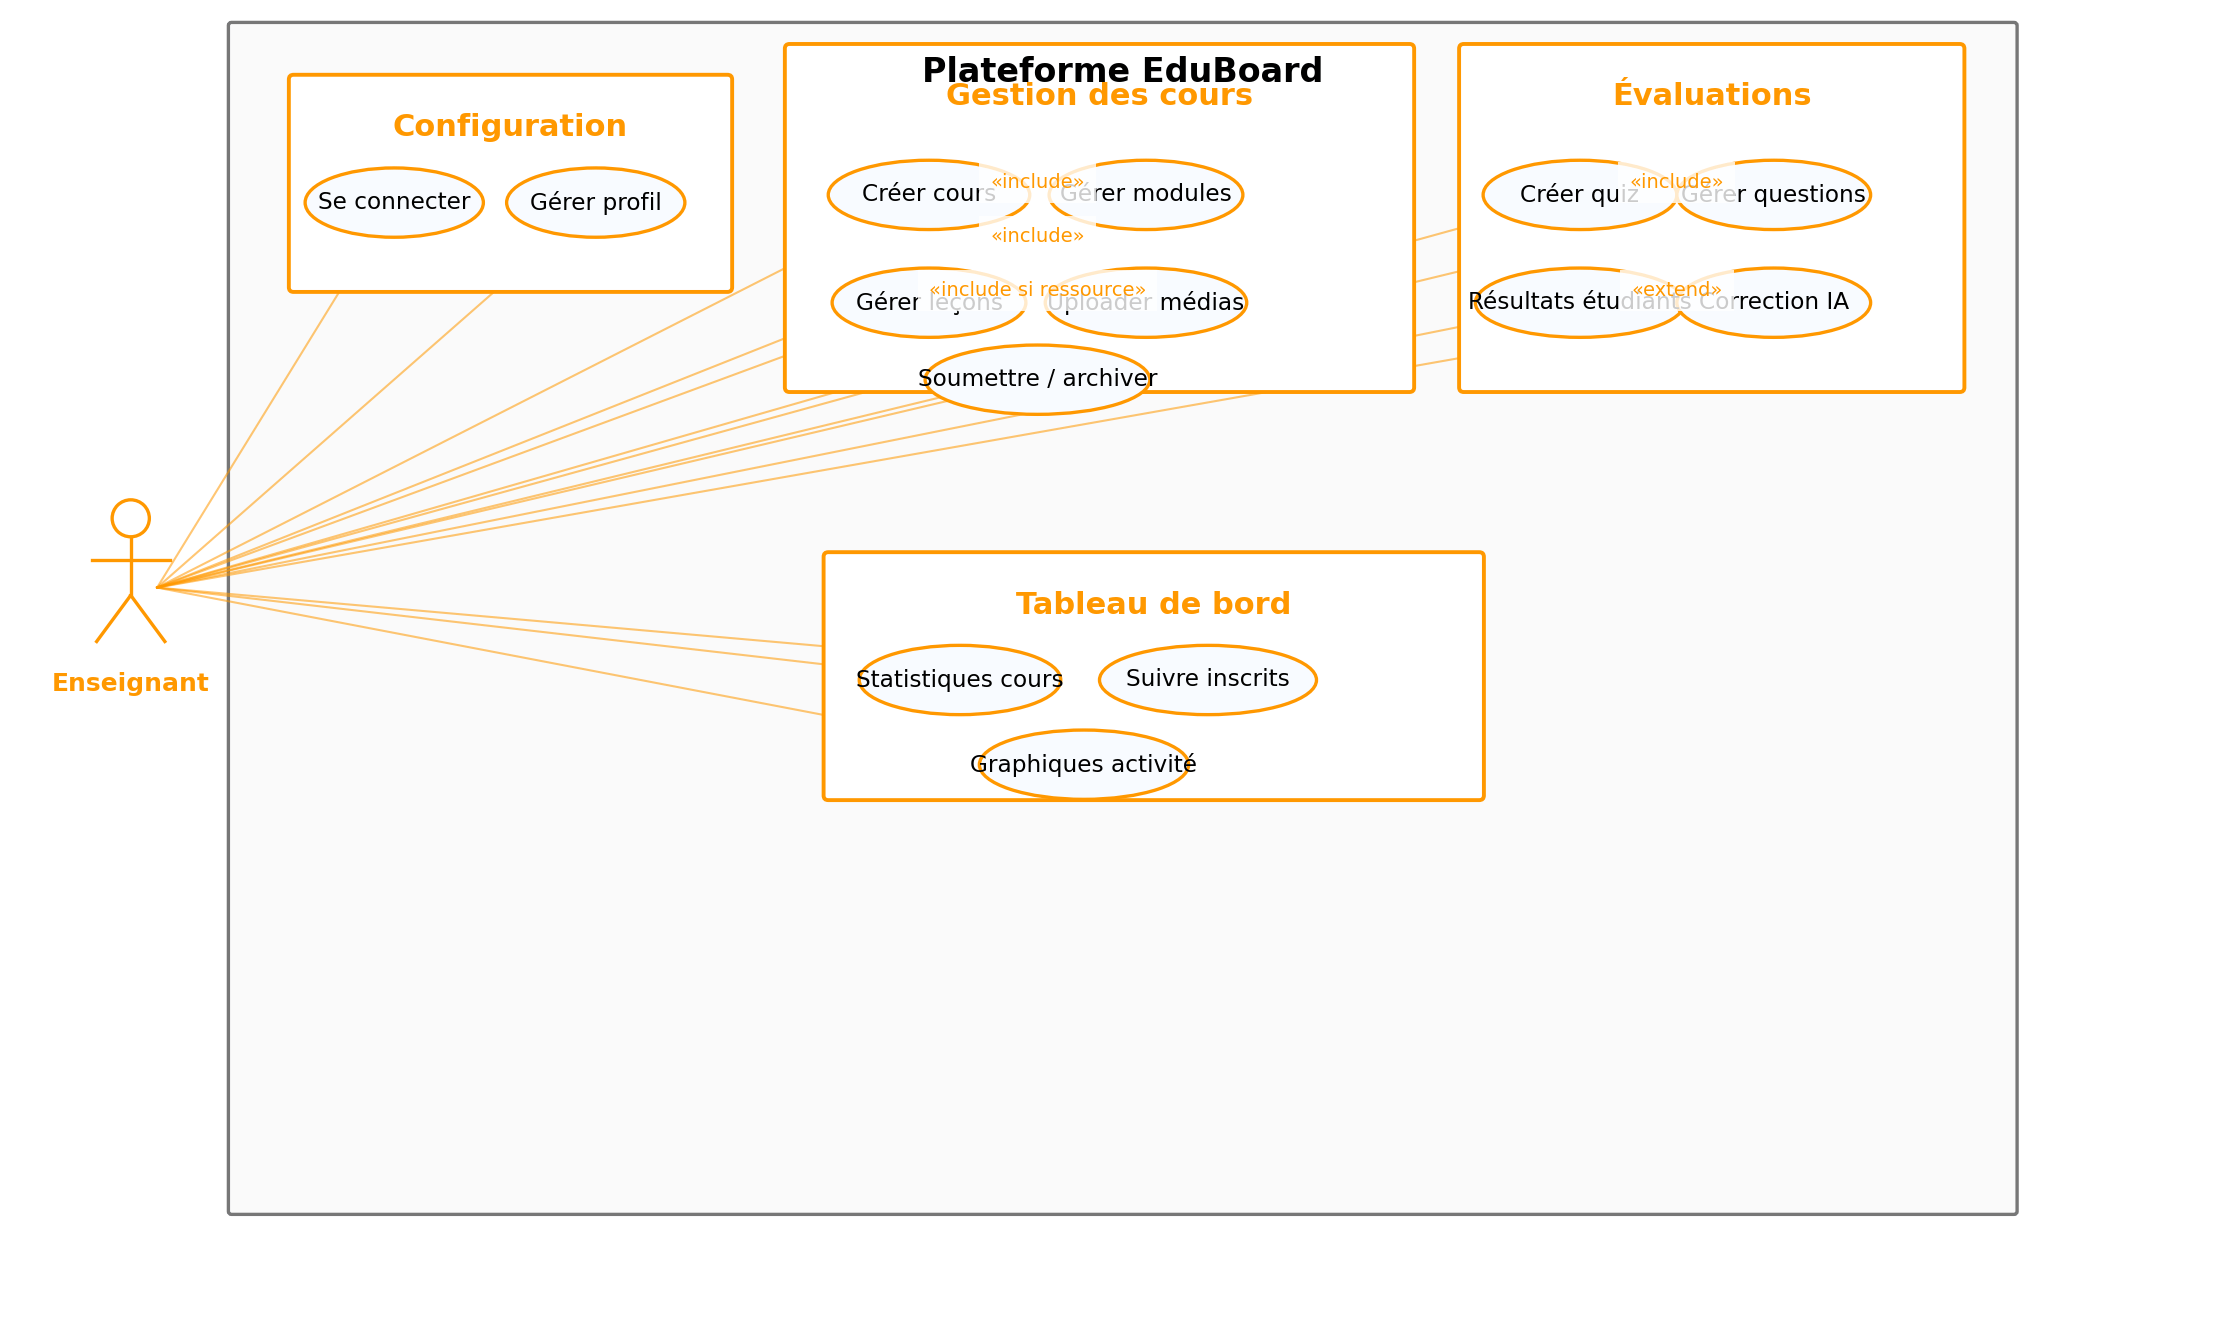
\includegraphics[width=\textwidth]{DIAGRAMME_DE_CAS_D_UTILISATION_-_ENSEIGNANT.png}
  \caption{Diagramme de cas d'utilisation – Espace Enseignant}
  \label{fig:uc_enseignant}
\end{figure}
\noindent  Ce diagramme représente le périmètre fonctionnel de l'acteur \textbf{Enseignant}, responsable de la création et de la gestion du contenu pédagogique au sein de la plateforme \textbf{EduBoard}. Il illustre les principales interactions de l'enseignant avec son espace dédié ainsi que son rôle dans l'organisation des formations.

\medskip

\noindent  Définir les responsabilités de l'enseignant dans le cycle de vie des cours, depuis leur création jusqu'au suivi des apprenants, afin de préciser les fonctionnalités qui lui sont accessibles.

\medskip

\noindent  L'enseignant peut créer et gérer des cours, organiser leur contenu en chapitres et leçons, importer des ressources pédagogiques, concevoir des quiz, publier ou dépublier des contenus, consulter les statistiques de ses formations et gérer son profil personnel.

\medskip

\noindent  Ce diagramme met en évidence les fonctionnalités dédiées aux enseignants et justifie l'architecture de gestion des contenus pédagogiques ainsi que les mécanismes de suivi des apprenants implémentés dans la plateforme.


\subsection{Diagramme de Cas d'Utilisation – Administrateur}

\begin{figure}[H]
  \centering
  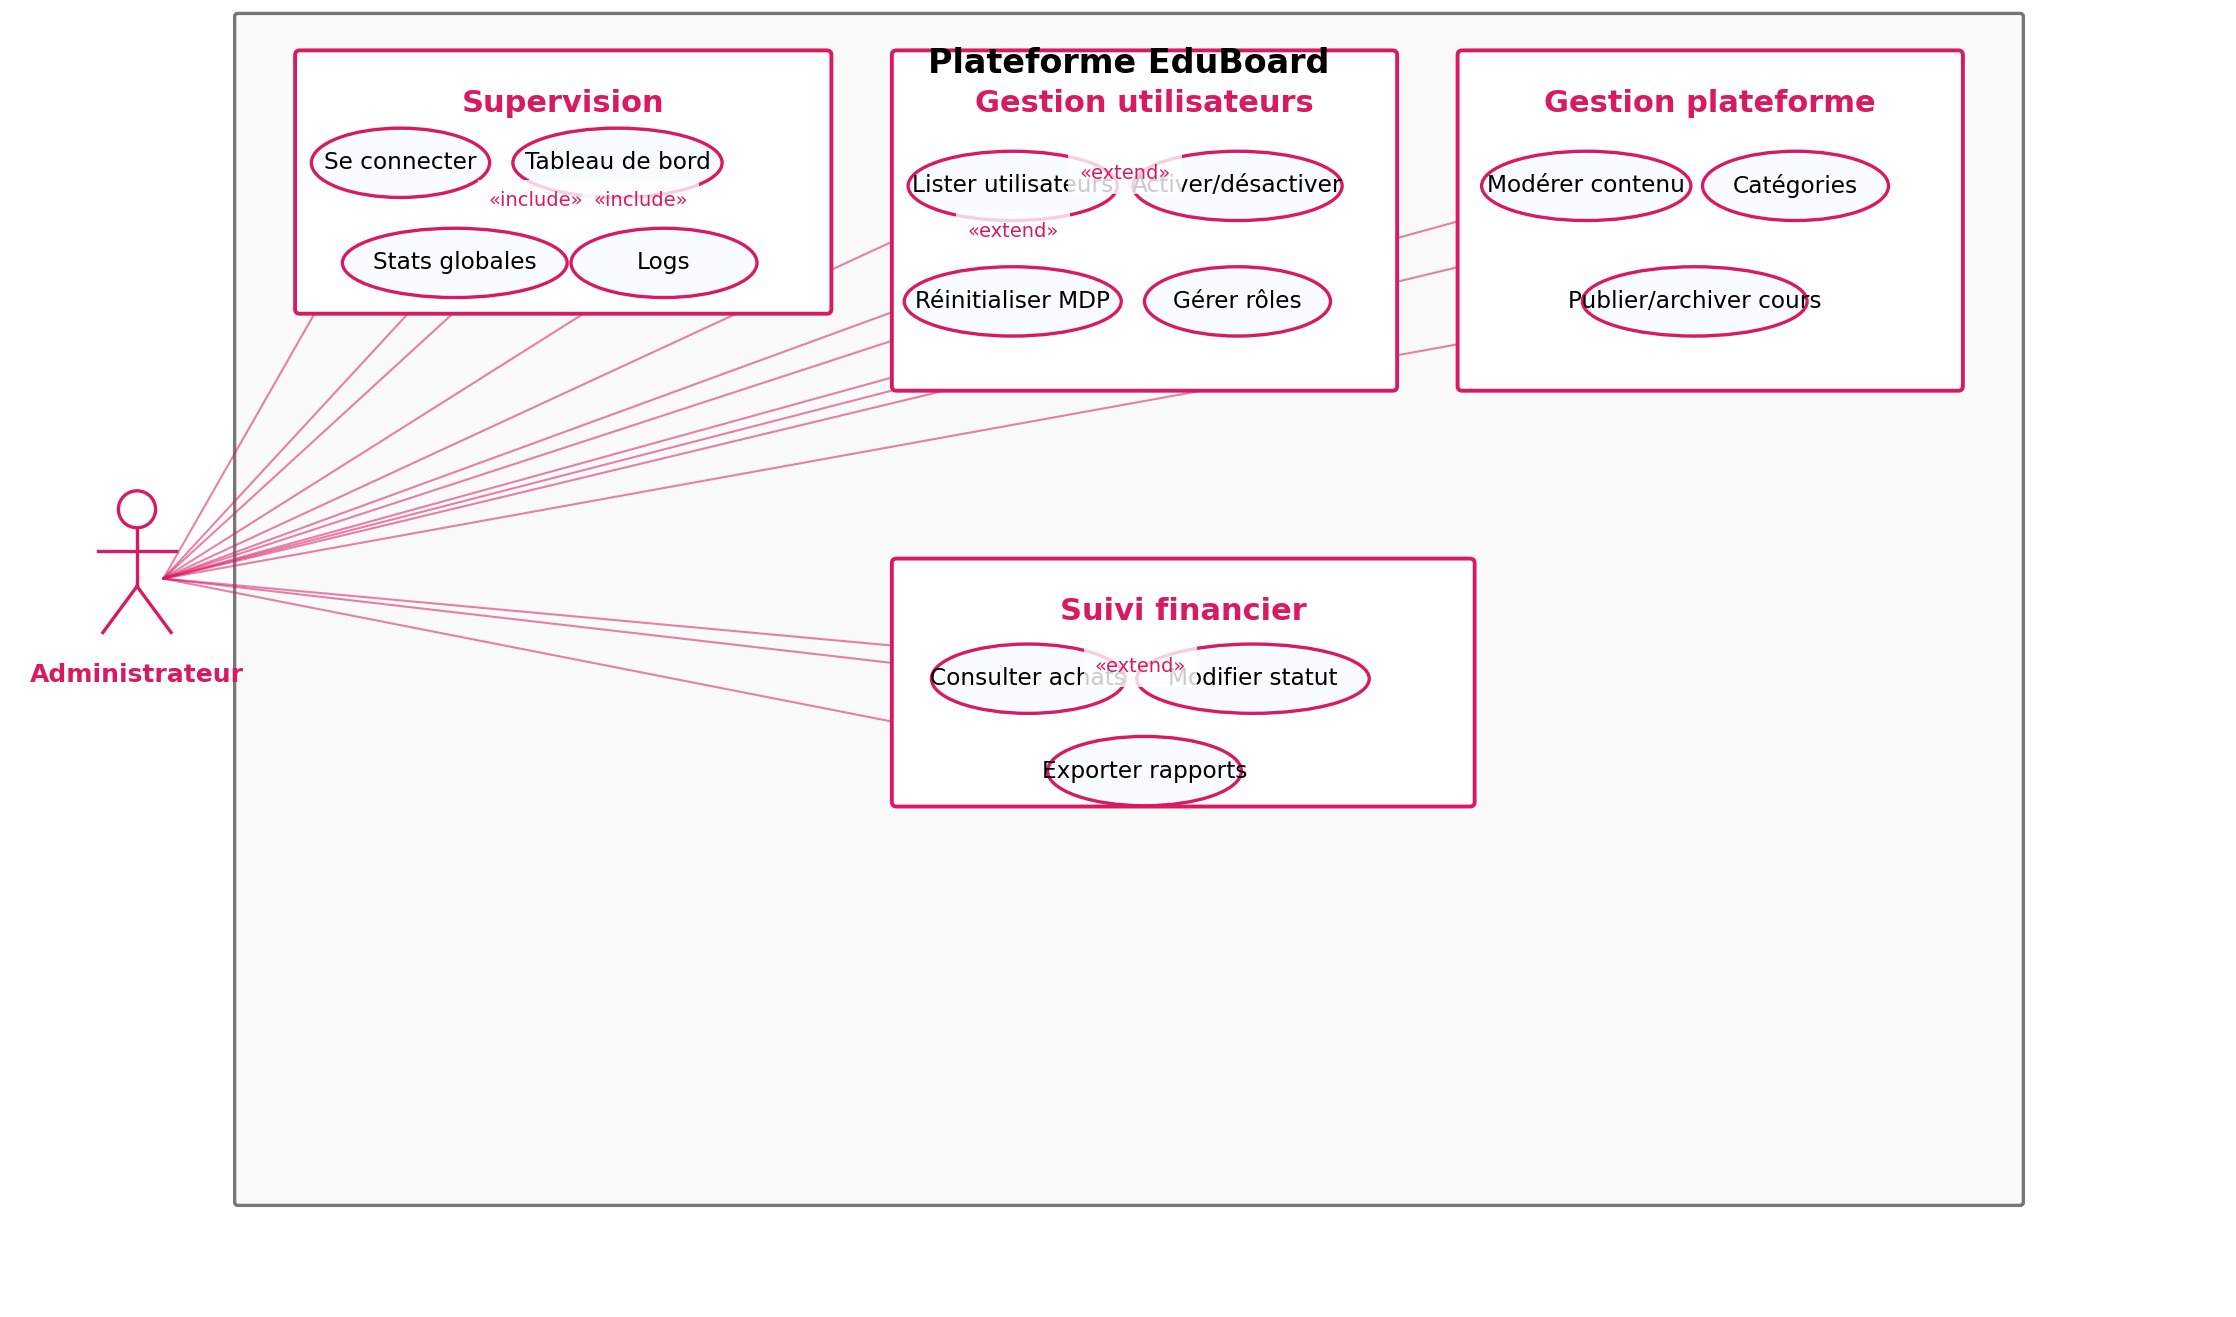
\includegraphics[width=\textwidth]{DIAGRAMME_DE_CAS_D_UTILISATION_-_ADMINISTRATEUR.png}
  \caption{Diagramme de cas d'utilisation – Espace Administrateur}
  \label{fig:uc_admin}
\end{figure}
\noindent  Ce diagramme représente le périmètre fonctionnel de l'acteur \textbf{Administrateur}, chargé de la supervision et de la gouvernance de la plateforme \textbf{EduBoard}. Il offre une vision globale des fonctionnalités de contrôle et de gestion accessibles depuis son tableau de bord.

\medskip

\noindent  Définir les responsabilités de l'administrateur en matière de gestion des utilisateurs, de supervision des contenus, de suivi des transactions et d'accès aux statistiques globales de la plateforme.

\medskip

\noindent  L'administrateur peut gérer les comptes utilisateurs et leurs rôles, modérer les contenus publiés, consulter les statistiques globales de la plateforme, superviser les transactions et l'historique des achats, accéder aux informations de suivi des utilisateurs et configurer les paramètres généraux du système.

\medskip

\noindent  Ce diagramme justifie la mise en œuvre du contrôle d'accès basé sur les rôles (\textit{RBAC}) et garantit que les fonctionnalités administratives sont exclusivement réservées aux utilisateurs disposant des autorisations appropriées.


% ------------------------------------------------------------

\section{Besoins Fonctionnels}

\begin{table}[H]
\centering
\caption{Besoins fonctionnels de la plateforme EduBoard}
\label{tab:bf}
\renewcommand{\arraystretch}{1.3}

\begin{tabularx}{\textwidth}{|p{4cm}|X|}
\hline
\textbf{Module} & \textbf{Fonctionnalités} \\
\hline

Gestion des utilisateurs et authentification &
Inscription des utilisateurs, connexion avec jeton \ac{JWT}, réinitialisation du mot de passe, gestion du profil, activation ou désactivation des comptes par l'administrateur et redirection selon le rôle utilisateur. \\
\hline

Gestion des cours, chapitres et leçons &
Création et gestion des cours, organisation hiérarchique (Cours $\rightarrow$ Chapitres $\rightarrow$ Leçons), ajout de contenus pédagogiques (vidéos, articles, PDF), importation de fichiers, publication des chapitres et gestion de la progression séquentielle. \\
\hline

Évaluation et quiz intelligents &
Création de quiz, passage des évaluations par les étudiants, correction automatique, calcul des scores, génération de feedback personnalisé par l'\ac{IA}, conservation de l'historique des tentatives et quiz de positionnement. \\
\hline

Suivi, progression et recommandations &
Suivi de la progression des apprenants, calcul des taux de complétion, recommandations personnalisées, apprentissage adaptatif et génération automatique de certificats PDF. \\
\hline

Paiement et commerce &
Achat de cours payants, gestion des transactions et des statuts de paiement, consultation de l'historique des achats, envoi des confirmations par email et gestion des remboursements. \\
\hline

Chatbot pédagogique IA &
Assistant conversationnel intégré accessible depuis toutes les pages, réponses contextualisées selon le parcours de l'étudiant et conservation de l'historique des échanges durant la session. \\
\hline

\end{tabularx}
\end{table}



% ------------------------------------------------------------

\begin{table}[H]
\centering
\caption{Besoins non fonctionnels de la plateforme EduBoard}
\label{tab:bnf}

\renewcommand{\arraystretch}{1.2}

\begin{tabularx}{\textwidth}{|p{3.5cm}|X|}
\hline
\textbf{Critère} & \textbf{Exigence} \\
\hline

Performance &
Temps de réponse inférieur à 2 secondes pour les opérations standard et inférieur à 500 ms pour les lectures simples. \\
\hline

Sécurité &
Authentification JWT, utilisation obligatoire du protocole HTTPS et hachage des mots de passe avec BCrypt. \\
\hline

Scalabilité &
Architecture orientée services avec séparation Frontend/Backend et conteneurisation Docker. \\
\hline

Disponibilité &
Taux de disponibilité cible supérieur à 99\% en environnement de production. \\
\hline

Compatibilité &
Interface responsive compatible avec Chrome, Firefox, Safari ainsi que les plateformes iOS et Android. \\
\hline

Upload fichiers &
Prise en charge de l'importation de vidéos jusqu'à 500 MB via Azure Blob Storage. \\
\hline

Maintenabilité &
Architecture Controller--Service--Repository avec injection de dépendances. \\
\hline

\ac{CORS} &
Origines autorisées : \texttt{localhost:3000} et \texttt{localhost:5173}. \\
\hline

Documentation \ac{API} &
Documentation Swagger/OpenAPI intégrée et accessible via \texttt{/swagger}. \\
\hline

\end{tabularx}
\end{table}



% ------------------------------------------------------------
\section{Description des Scénarios Principaux}

\begin{table}[H]
  \centering
  \caption{Description textuelle du cas d'utilisation « Acheter un cours »}
  \label{tab:sc_achat}
  \begin{tabularx}{\textwidth}{|l|X|}
    \hline
    Acteur principal  & Étudiant \\
    \hline
    Préconditions     & Étudiant authentifié, cours non encore acheté \\
    \hline
    Scénario nominal  &
      1.~L'étudiant voit le bouton « Acheter » sur le cours payant.\newline
      2.~Il clique \textrightarrow{} POST \texttt{/api/purchase/initiate}.\newline
      3.~Le backend crée un achat en statut « Pending ».\newline
      4.~Flouci retourne une URL de paiement.\newline
      5.~Redirection vers la page Flouci.\newline
      6.~Après paiement~: GET \texttt{/api/purchase/\{id\}/verify}.\newline
      7.~Statut passe à « Completed », email envoyé. \\
    \hline
    Alt. 1            & Flouci non configuré (dev)~: simulation automatique \\
    \hline
    Alt. 2            & Paiement refusé~: statut « Failed » \\
    \hline
    Postconditions    & Accès au cours débloqué, chapitre 1 accessible \\
    \hline
  \end{tabularx}
\end{table}


\subsection{Scénario : Acheter un cours}

\begin{table}[H]
  \centering
  \caption{Description textuelle du cas d'utilisation « Acheter un cours »}
  \label{tab:sc_achat}
  \begin{tabularx}{\textwidth}{|l|X|}
    \hline
    Acteur principal  & Étudiant \\
    \hline
    Préconditions     & Étudiant authentifié, cours non encore acheté \\
    \hline
    Scénario nominal  &
      1.~L'étudiant voit le bouton « Acheter » sur le cours payant.\newline
      2.~Il clique \textrightarrow{} POST \texttt{/api/purchase/initiate}.\newline
      3.~Le backend crée un achat en statut « Pending ».\newline
      4.~Flouci retourne une URL de paiement.\newline
      5.~Redirection vers la page Flouci.\newline
      6.~Après paiement~: GET \texttt{/api/purchase/\{id\}/verify}.\newline
      7.~Statut passe à « Completed », email envoyé. \\
    \hline
    Alt. 1            & Flouci non configuré (dev)~: simulation automatique \\
    \hline
    Alt. 2            & Paiement refusé~: statut « Failed » \\
    \hline
    Postconditions    & Accès au cours débloqué, chapitre 1 accessible \\
    \hline
  \end{tabularx}
\end{table}

\subsection{Scénario : Progresser dans un chapitre}

\begin{table}[H]
  \centering
  \caption{Description textuelle du cas d'utilisation « Progresser dans un chapitre »}
  \label{tab:sc_progression}
  \begin{tabularx}{\textwidth}{|l|X|}
    \hline
    Acteur principal  & Étudiant \\
    \hline
    Préconditions     & Étudiant inscrit au cours, chapitre précédent complété \\
    \hline
    Scénario nominal  &
      1.~L'étudiant clique sur le chapitre $N$.\newline
      2.~POST \texttt{/api/chapters/\{id\}/access} -- l'\ac{IA} enregistre l'accès.\newline
      3.~Le système vérifie le déverrouillage.\newline
      4.~L'étudiant consulte les leçons et télécharge les \ac{PDF}s.\newline
      5.~Toutes les 30\,s~: PUT \texttt{/api/chapters/\{id\}/time}.\newline
      6.~L'étudiant passe le quiz \textrightarrow{} feedback \ac{IA}.\newline
      7.~POST \texttt{/api/chapters/\{id\}/complete} \textrightarrow{} chapitre validé.\newline
      8.~Si dernier chapitre~: certificat \ac{PDF} généré automatiquement. \\
    \hline
    Alt. 1            & Chapitre précédent non complété~: message de verrouillage \\
    \hline
    Alt. 2            & Quiz non réussi~: message d'encouragement, nouvelle tentative \\
    \hline
    Postconditions    & \texttt{ChapterProgress} mis à jour, chapitre $N+1$ déverrouillé \\
    \hline
  \end{tabularx}
\end{table}
\section*{Conclusion}
\addcontentsline{toc}{section}{Conclusion}

Ce chapitre a permis l'identification et la formalisation rigoureuse de toutes les
exigences fonctionnelles et non fonctionnelles de la plateforme EduBoard. La
modélisation \ac{UML} jette les bases solides de la conception détaillée présentée dans le chapitre suivant.

% ============================================================
%  08_chapitre3_conception.tex  –  Chapitre 3 : Conception de la Solution
% ============================================================
\chapter{Conception de la Solution}

\section*{Introduction}
\addcontentsline{toc}{section}{Introduction}

Ce chapitre décrit l'architecture globale d'EduBoard et sa conception détaillée. Nous
présentons les choix architecturaux justifiés, le modèle de données, les diagrammes
d'activité, de séquence, les diagrammes de classes et de déploiement.
% ------------------------------------------------------------
\section{Architecture Globale}

EduBoard adopte une architecture en couches assurant une séparation claire des responsabilités.

\begin{table}[H]
  \centering
  \caption{Architecture N-Tiers de la plateforme EduBoard}
  \label{tab:architecture}
  \renewcommand{\arraystretch}{1.3}
  \begin{tabularx}{\textwidth}{>{\raggedright\arraybackslash}p{3.5cm} p{4cm} X}
    \toprule
    \textbf{Couche} & \textbf{Technologie} & \textbf{Rôle} \\
    \midrule
    Présentation & React.js 18 (\ac{SPA}) & Interface utilisateur, routage client, gestion de l'état \\
    API / Métier & ASP.NET Core 8 \ac{REST} & Logique métier, controllers, services, injection de dépendances \\
    Données & PostgreSQL 15 + EF Core 8 & Persistance, \ac{ORM}, migrations automatiques \\
    Stockage médias & Local \texttt{persistent\_uploads} & Stockage des PDFs, vidéos et images \\
    IA / Ext. & Anthropic, Groq, Flouci, SMTP & Feedback quiz, chatbot, paiement et emails \\
    \bottomrule
  \end{tabularx}
\end{table}

% ------------------------------------------------------------
\section{Diagrammes d'Activité}

\subsection{Diagramme d'Activité – Inscription et Authentification}

\begin{figure}[H]
  \centering
  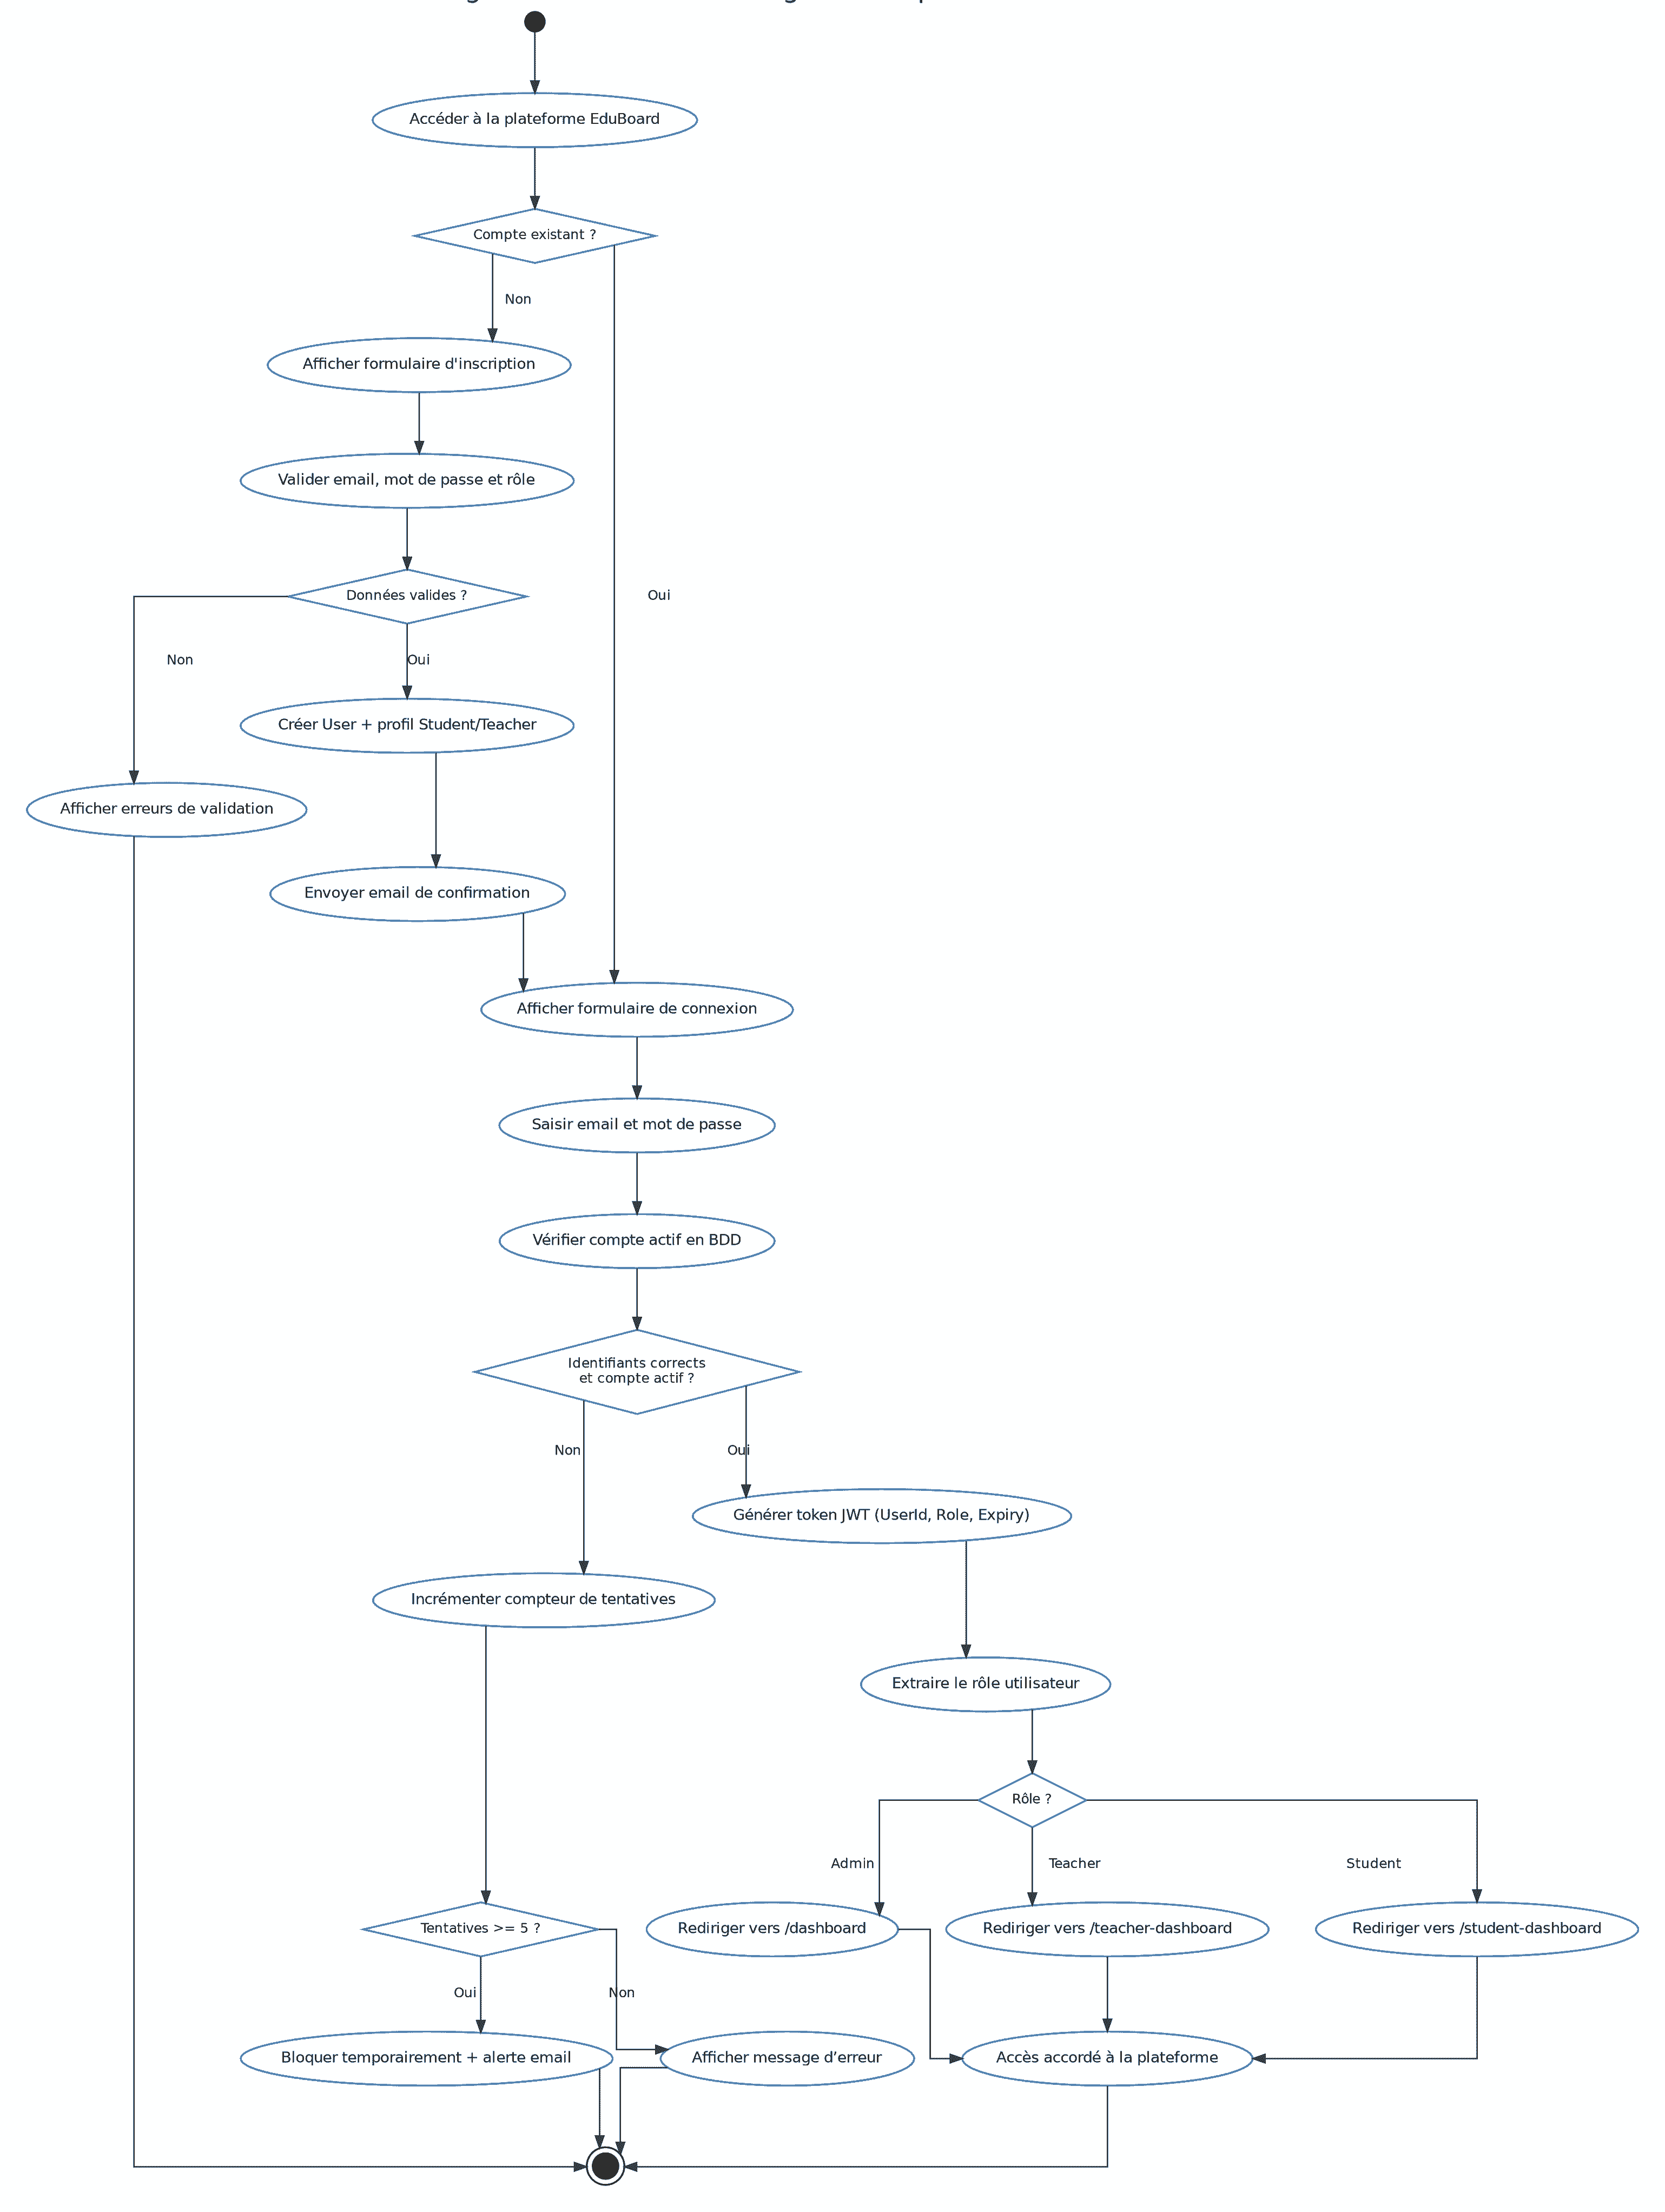
\includegraphics[height=0.8\textheight,keepaspectratio]{DIAGRAMME_D_ACTIVITE_-_INSCRIPTION_ET_AUTHENTIFICATION.png}
  \caption{Diagramme d'activité – Inscription et Authentification}
  \label{fig:act_auth}
\end{figure}
\noindent  Ce diagramme modélise le processus d’authentification et d’inscription sur la plateforme EduBoard, point d’entrée de l’application permettant l’accès sécurisé aux services. Il décrit le parcours d’un utilisateur depuis l’inscription ou la connexion jusqu’à l’obtention d’un token JWT et la redirection vers le tableau de bord approprié selon son rôle.

\noindent Il met en évidence la validation des données, la sécurisation des mots de passe via BCrypt, la génération d’un JWT et la gestion des cas d’erreur, tout en assurant une authentification stateless adaptée à une architecture scalable.
\subsection{Diagramme d'Activité – Achat d'un Cours}

\begin{figure}[H]
  \centering
   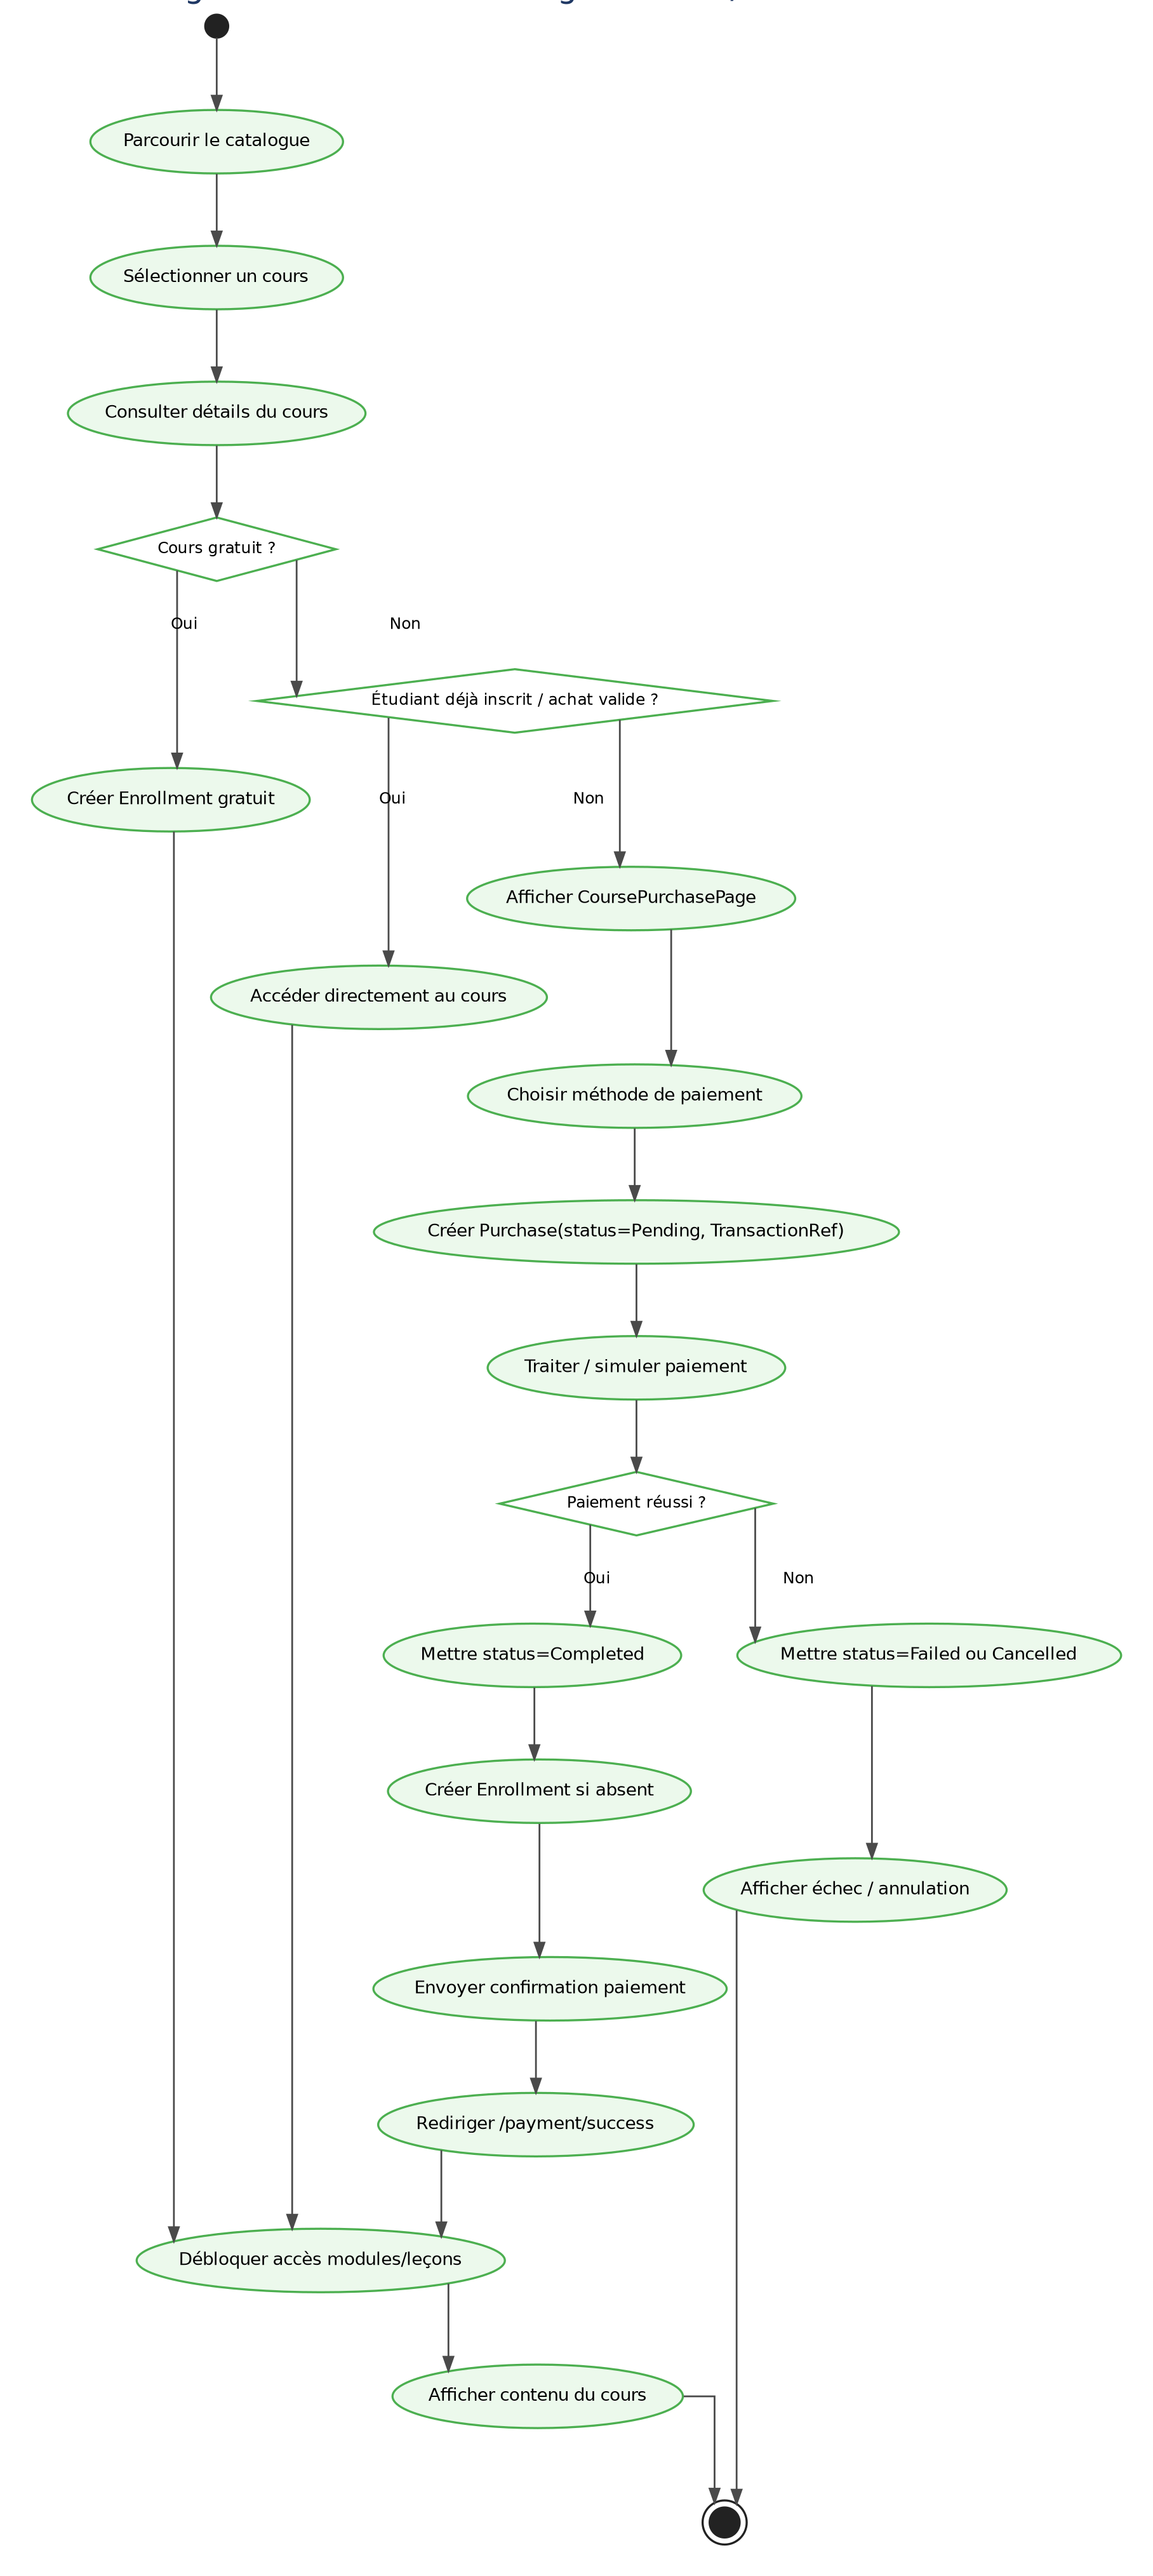
\includegraphics[height=0.8\textheight,keepaspectratio]{DIAGRAMME_D_ACTIVITE_-_ACHAT_D_UN_COURS.png}
  \caption{Diagramme d'activité – Processus d'achat d'un cours}
  \label{fig:act_achat}
\end{figure}
\noindent   Ce diagramme modélise le processus commercial d’EduBoard, couvrant l’acquisition d’un cours payant via le système de paiement Flouci, depuis la consultation du catalogue jusqu’au déblocage de l’accès au contenu pédagogique. Il formalise les étapes du tunnel d’achat, la gestion des statuts de transaction (Pending, Completed, Failed, Cancelled), l’intégration de la passerelle de paiement Flouci avec redirection et callback, ainsi qu’un mode de simulation en environnement local. L’accès au contenu est conditionné à la validation du paiement, avec envoi automatique d’un email de confirmation et séparation claire entre contrôleur, service métier et service de notification.

\subsection{Diagramme d'Activité – Passage d'un Quiz}


\begin{figure}[H]
    \centering
    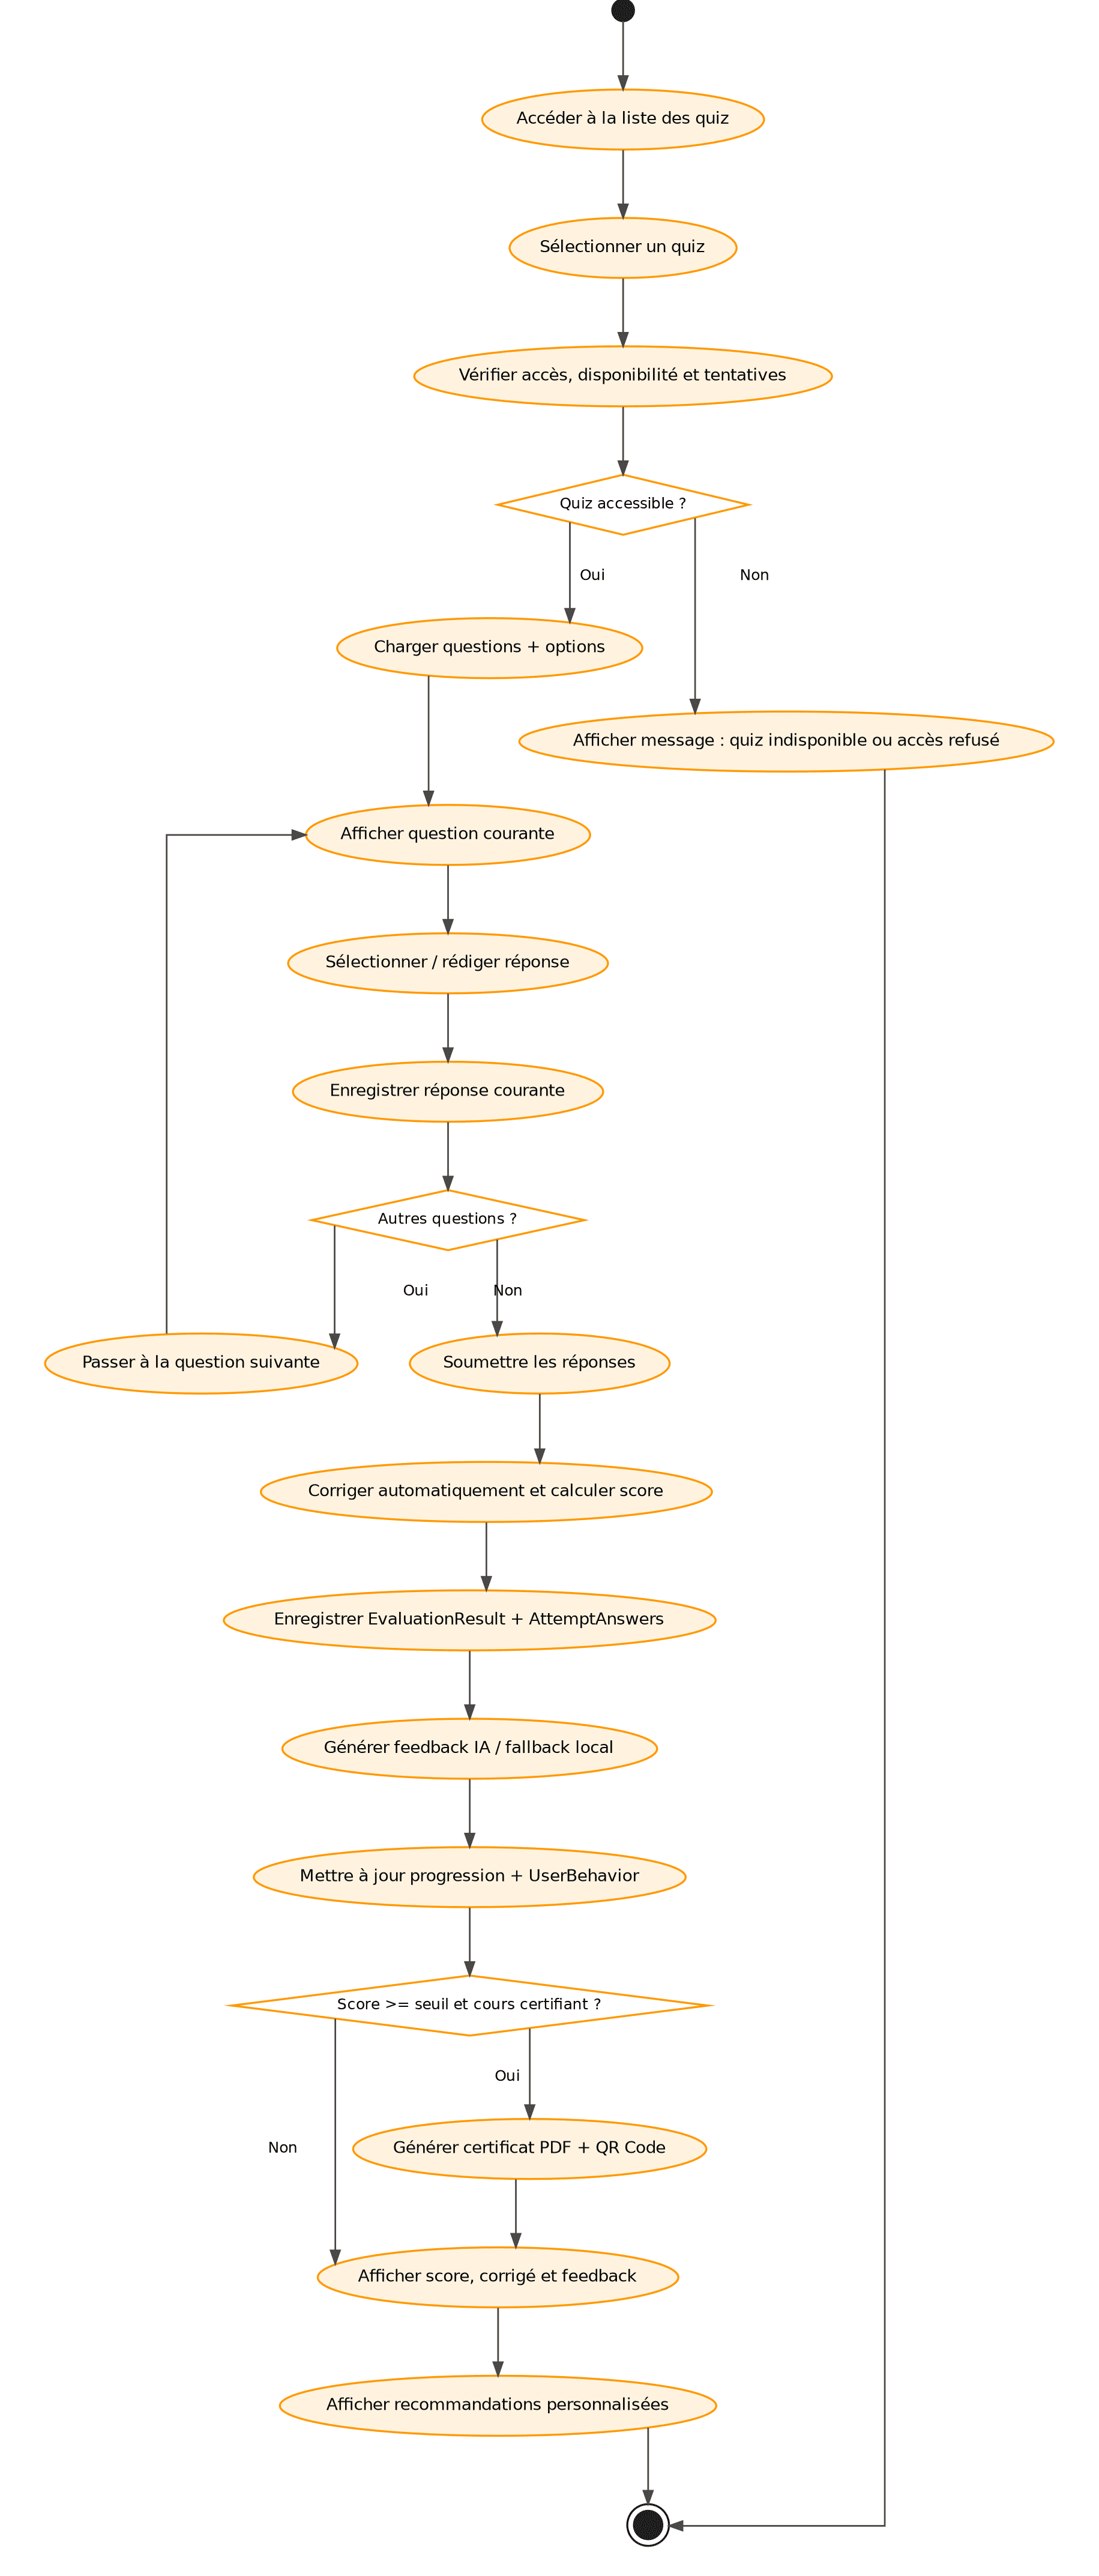
\includegraphics[height=0.8\textheight,keepaspectratio]{DIAGRAMME_D_ACTIVITE_-_PASSAGE_D_UN_QUIZ.png}
    \caption{Diagramme d'activité : Passage d'un quiz avec feedback IA}
    \label{fig:act_quiz}
\end{figure}
\noindent Ce diagramme modélise le processus d’évaluation des étudiants via les quiz adaptatifs d’EduBoard, incluant le déroulement d’un quiz et l’intégration de l’API Anthropic Claude pour générer un feedback pédagogique personnalisé. Il décrit le flux complet d’une tentative de quiz : accès avec vérification des droits et des limites, navigation question par question avec enregistrement des réponses, correction automatique et calcul du score, génération d’un feedback via \textit{QuizFeedbackService} (avec fallback local), mise à jour de la progression utilisateur, et déclenchement éventuel d’un certificat en cas de réussite. Ce processus permet de transformer une évaluation classique en un accompagnement pédagogique personnalisé basé sur l’IA.

\medskip

\noindent Ce diagramme met en évidence un processus central du système d’évaluation d’EduBoard, combinant correction automatique et génération de feedback intelligent afin d’améliorer l’apprentissage des étudiants.

% ------------------------------------------------------------
\section{Diagrammes de Séquence}

\subsection{Diagramme de Séquence – Authentification JWT}

\begin{figure}[H]
  \centering
  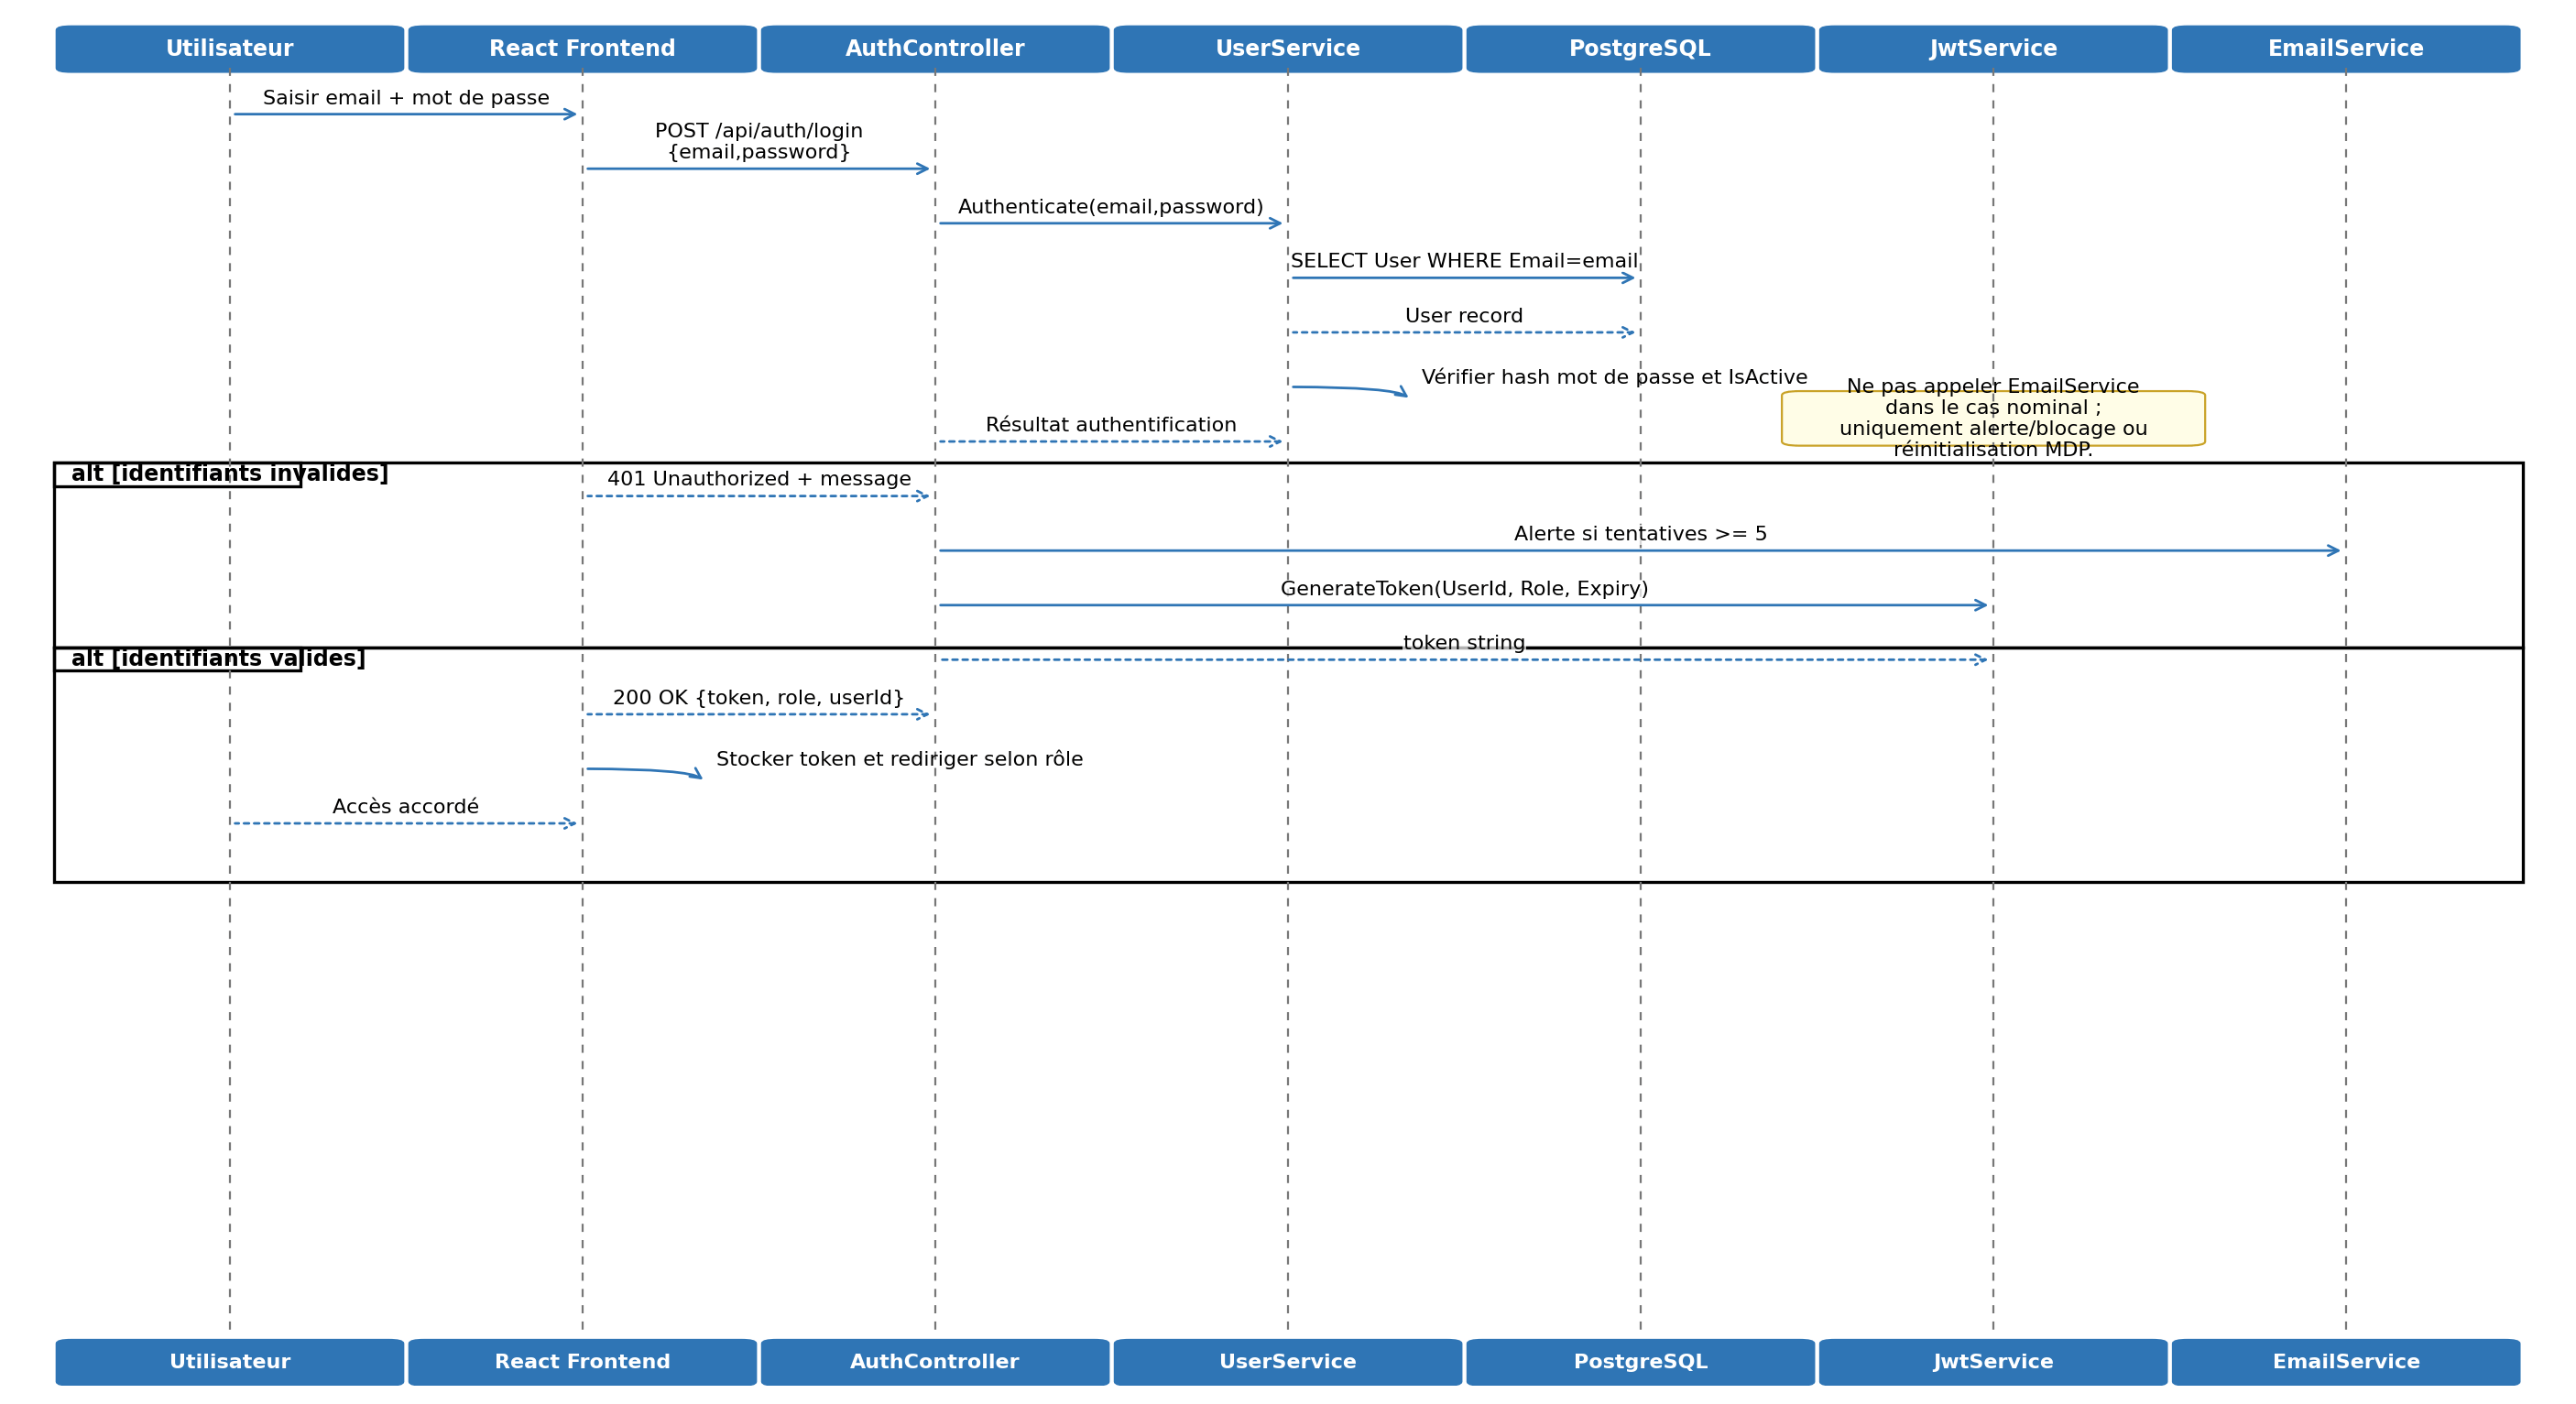
\includegraphics[width=\textwidth]{DIAGRAMME_DE_SEQUENCE_-_AUTHENTIFICATION_JWT.png}
  \caption{Diagramme de séquence – Authentification JWT}
  \label{fig:seq_auth}
\end{figure}
\noindent  Ce diagramme modélise le processus d’authentification basé sur JSON Web Token (JWT) dans EduBoard, illustrant les échanges entre le client React, l’API ASP.NET Core et la base de données lors d’une connexion.

\medskip

\noindent Il décrit le flux du endpoint \texttt{POST /api/auth/login}, depuis la soumission des identifiants jusqu’à la génération et l’utilisation du token JWT. Ce processus inclut la vérification des credentials, la création du token signé et son stockage côté client, ainsi que son injection automatique dans les requêtes protégées via le header \texttt{Authorization: Bearer}. Le diagramme met également en évidence les mécanismes de sécurité et la gestion des accès par rôle..
\subsection{Diagramme de Séquence – Achat d'un Cours}

\begin{figure}[H]
  \centering
  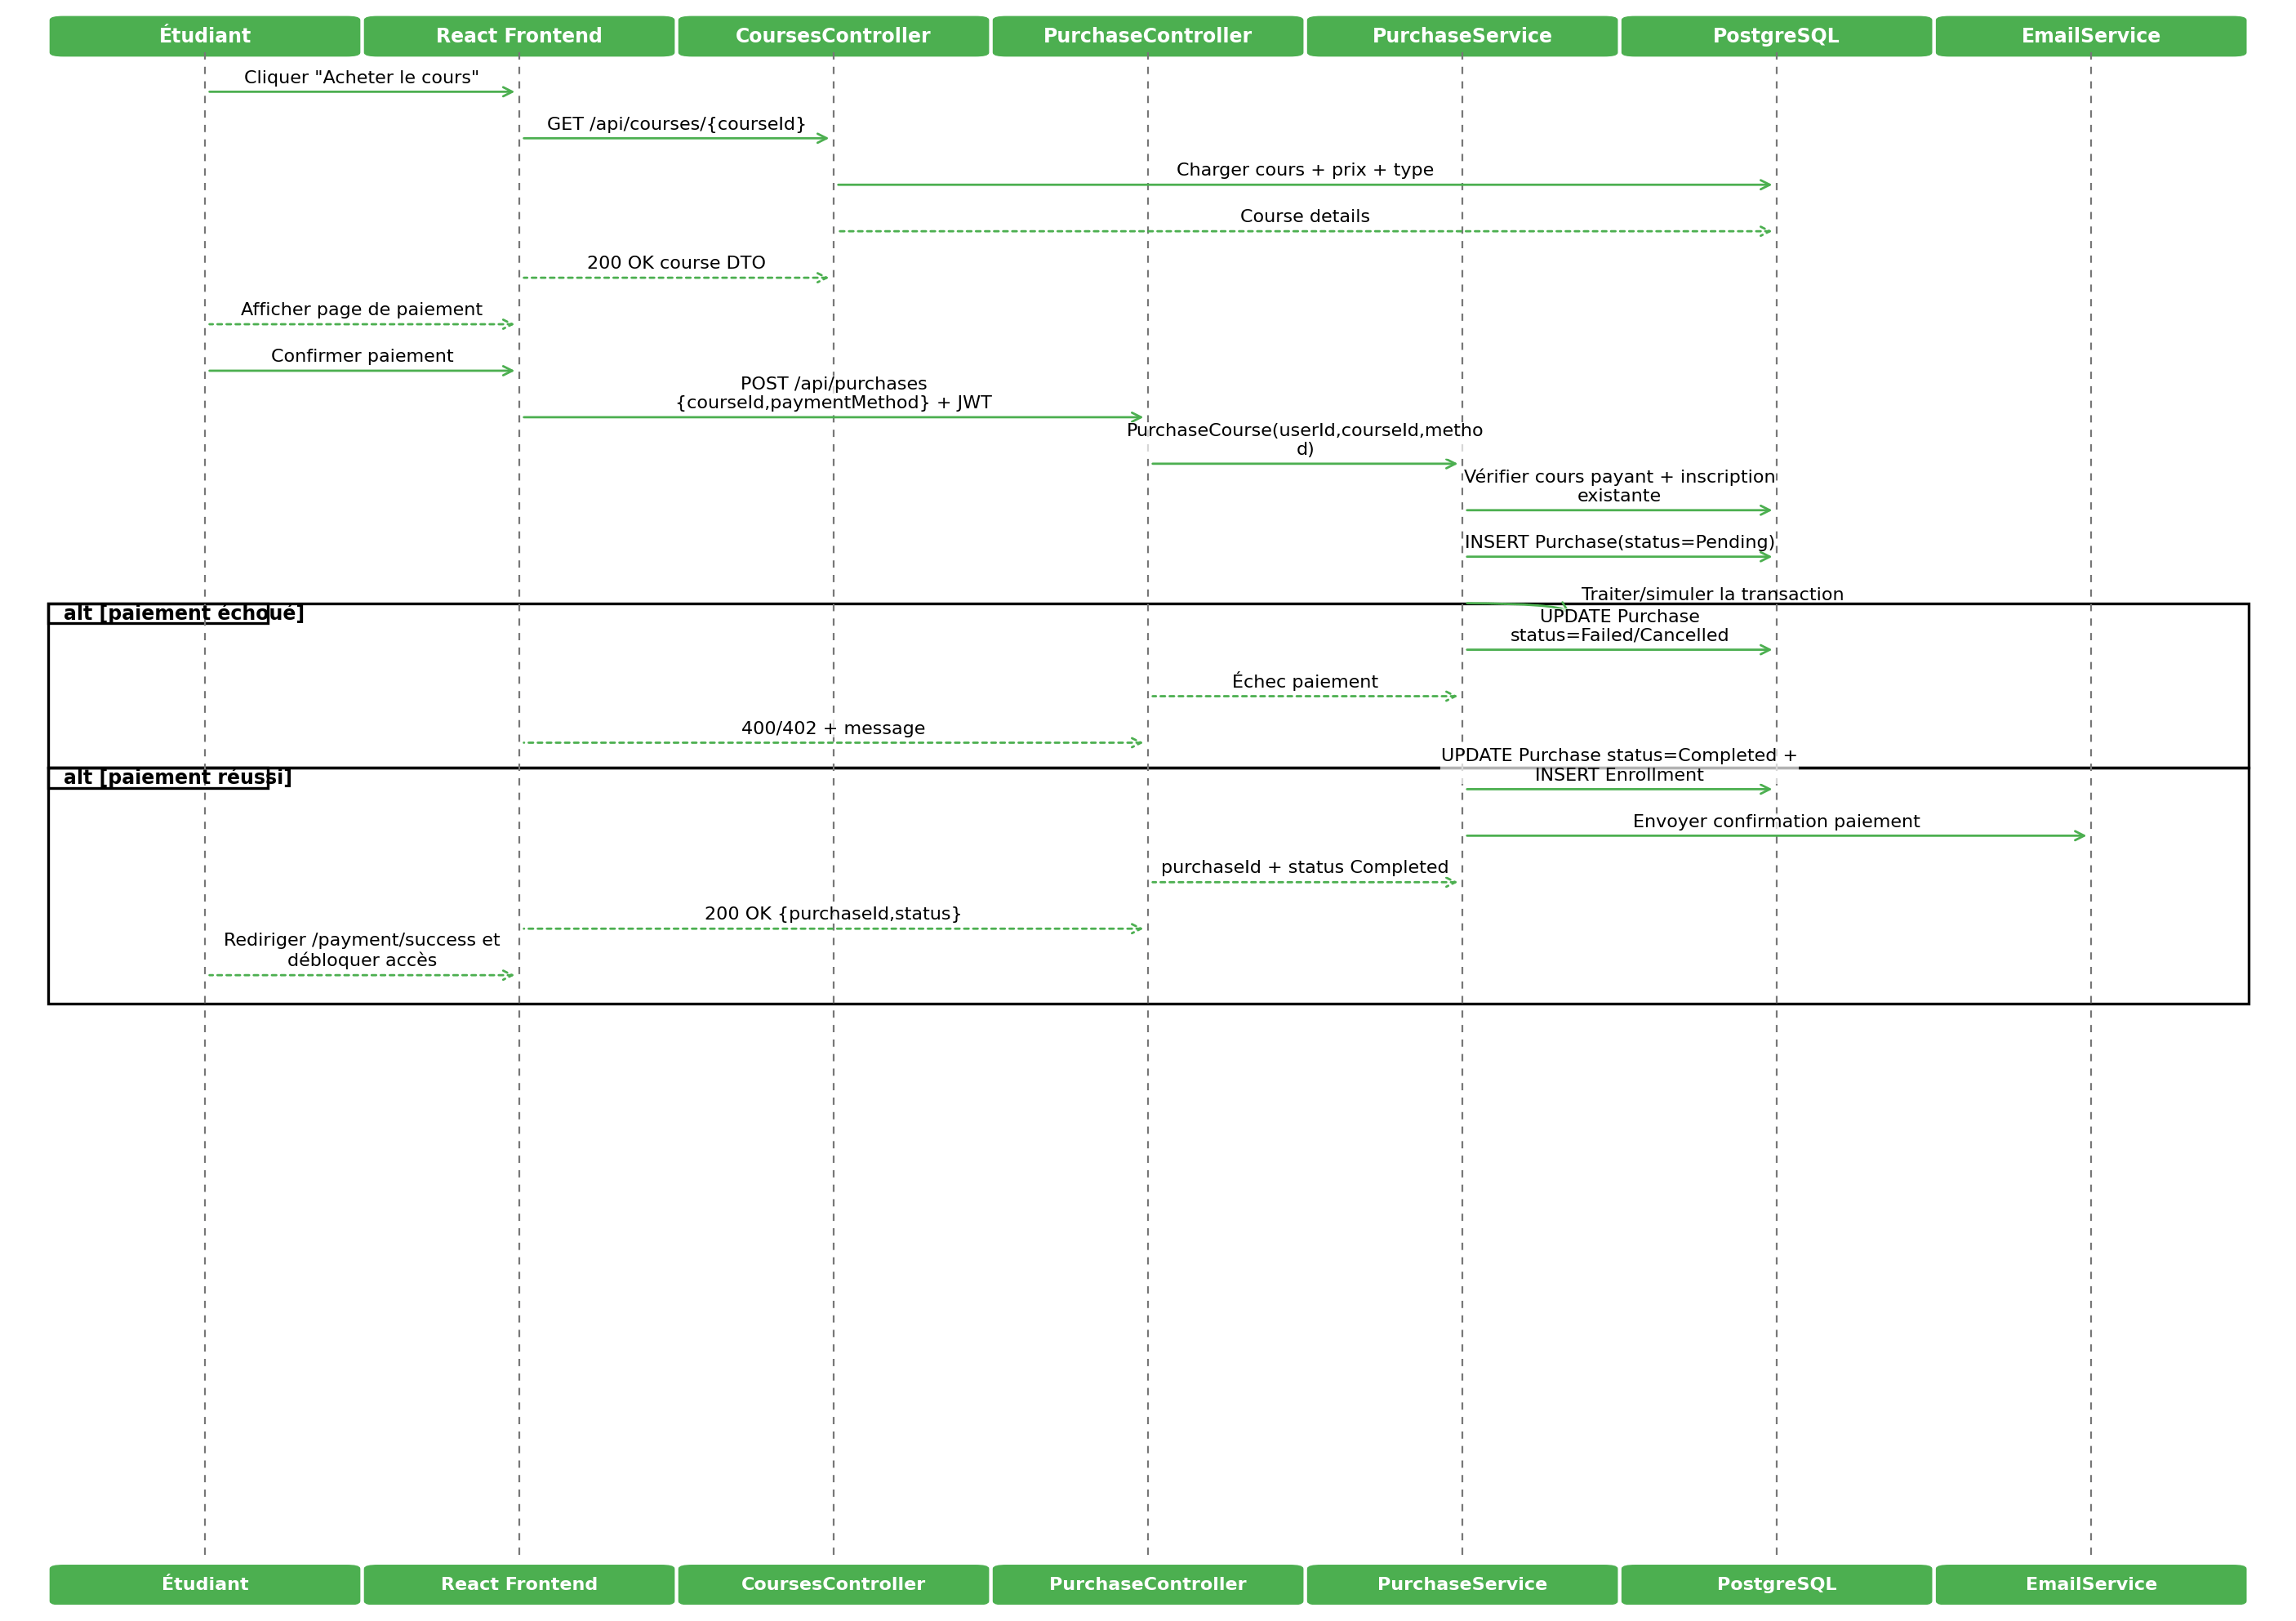
\includegraphics[width=\textwidth]{DIAGRAMME_DE_SEQUENCE_-_ACHAT_D_UN_COURS.png}
  \caption{Diagramme de séquence – Achat d'un cours}
  \label{fig:seq_achat}
\end{figure}
\noindent  Ce diagramme modélise le processus de paiement dans EduBoard, depuis l’initiation de l’achat jusqu’à la confirmation de l’accès au cours via la passerelle Flouci.

\medskip

\noindent Il décrit le flux du tunnel d’achat incluant la création d’une transaction en statut \textit{Pending}, la redirection vers Flouci, la vérification du paiement côté serveur, puis la validation finale permettant la création de l’inscription et l’envoi d’un email de confirmation. L’accès au cours n’est accordé qu’après validation effective du paiement.
\subsection{Diagramme de Séquence – Quiz avec Feedback IA}

\begin{figure}[H]
  \centering
  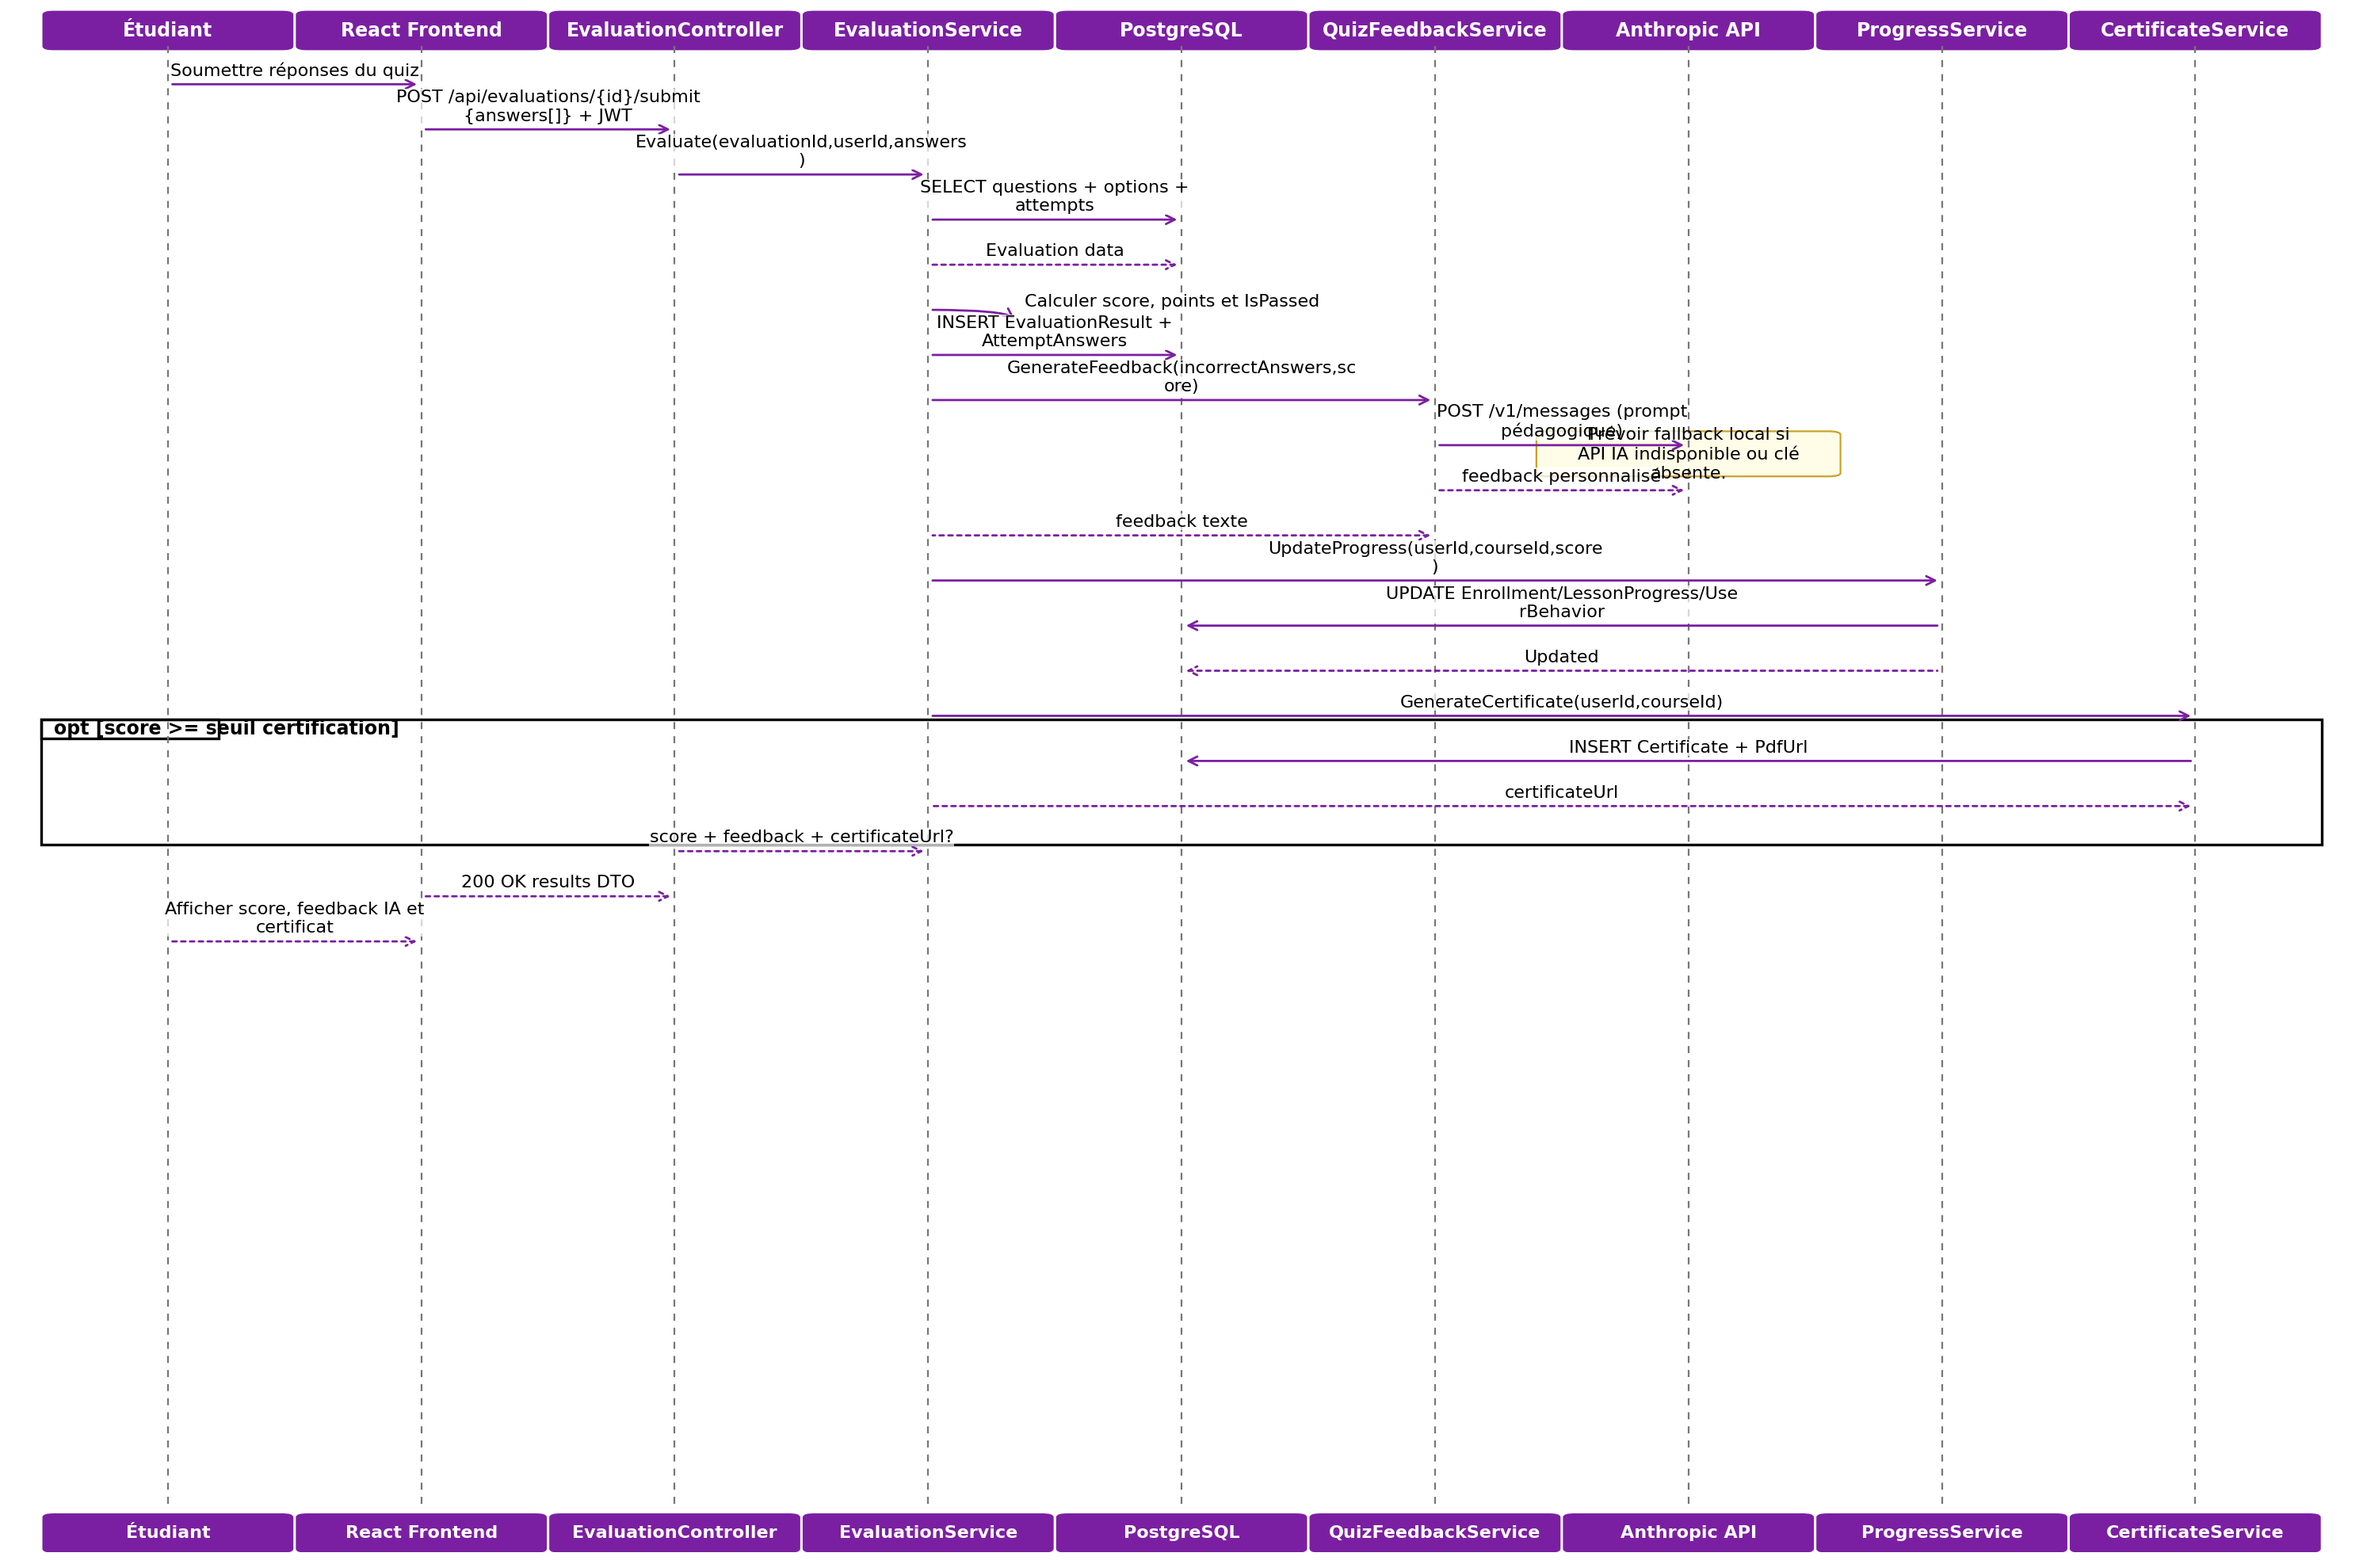
\includegraphics[width=\textwidth]{DIAGRAMME_DE_SEQUENCE_-_SOUMISSION_ET_FEEDBACK_IA_QUIZ.png}
  \caption{Diagramme de séquence – Soumission de quiz et feedback IA (Anthropic)}
  \label{fig:seq_quiz_ia}
\end{figure}
\noindent  Ce diagramme modélise la séquence d’interaction entre EduBoard et l’API Anthropic Claude pour la génération d’un feedback pédagogique personnalisé après la soumission d’un quiz, illustrant l’intégration de l’IA générative dans le cœur pédagogique de la plateforme. Il décrit le flux de traitement du endpoint \texttt{POST /api/quizzes/submit}, depuis la soumission des réponses jusqu’à l’affichage du feedback.

\medskip

\noindent Le processus inclut la correction automatique via \textit{EvaluationService}, la construction d’un prompt contextuel par \textit{QuizFeedbackService}, l’appel à l’API Anthropic (claude-sonnet), la réception et l’extraction du feedback, ainsi que sa persistance dans \texttt{QuizAttempt.AIFeedback}. En cas d’indisponibilité de l’API, un fallback local garantit la continuité du service avec un feedback générique basé sur le score.
\subsection{Diagramme de Séquence – Chatbot IA}

\begin{figure}[H]
  \centering
  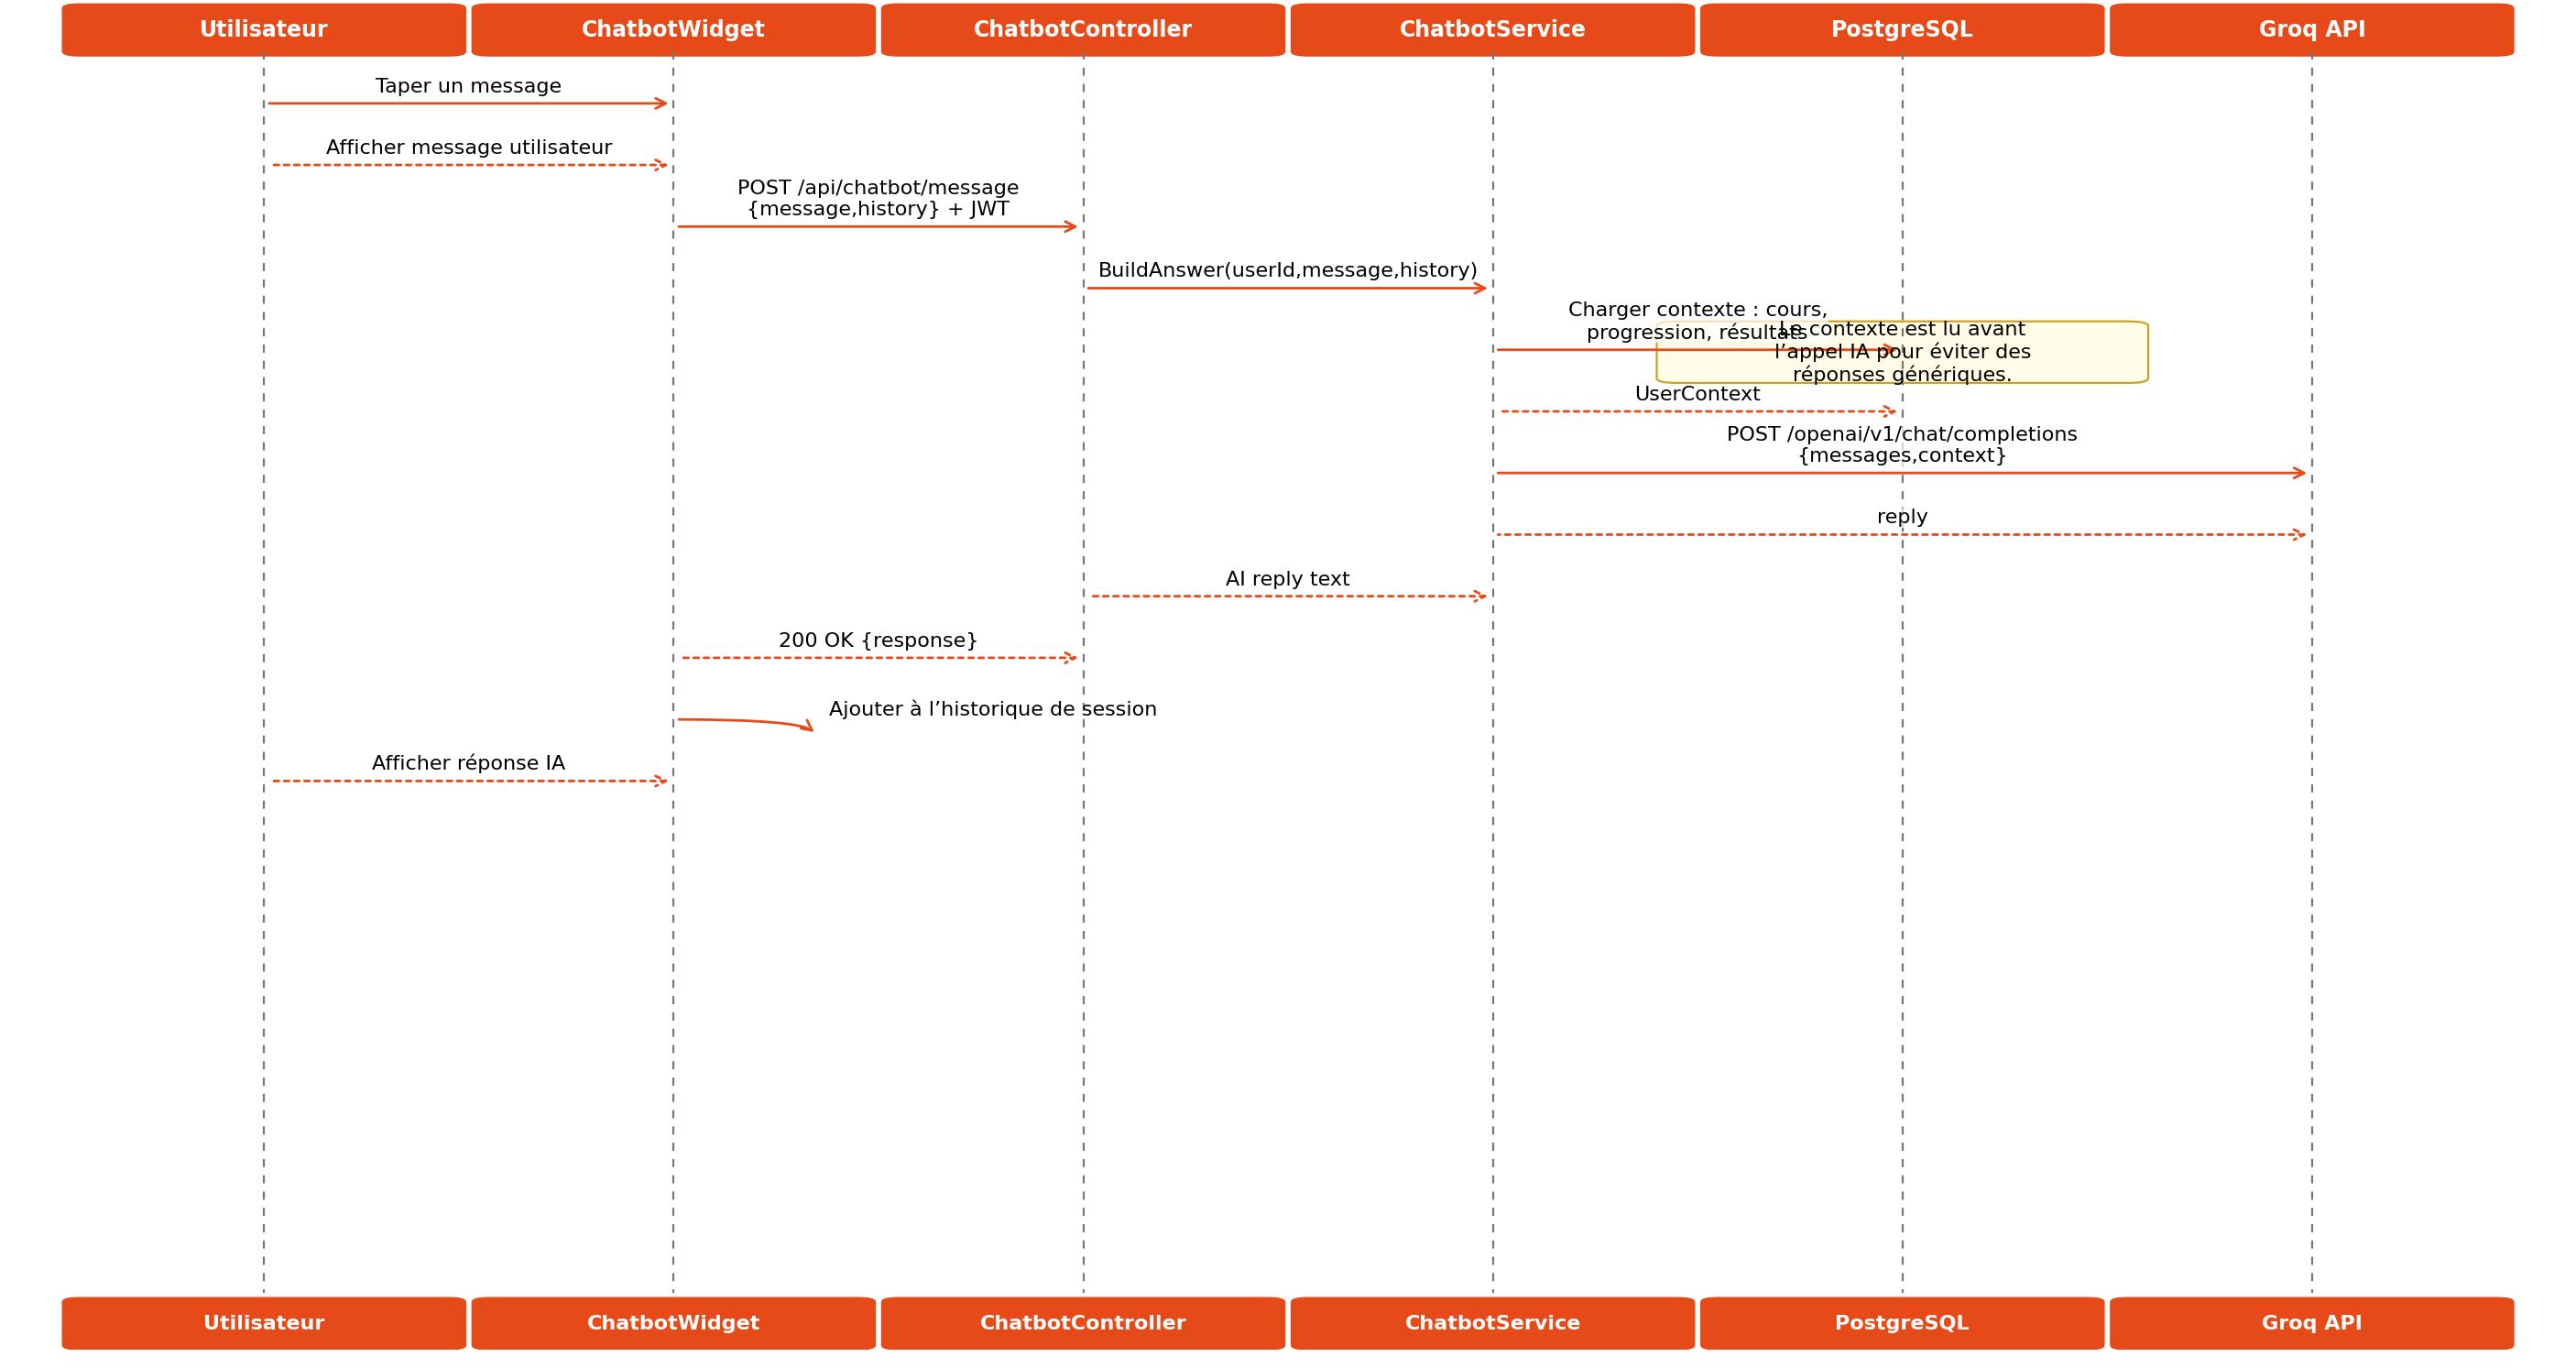
\includegraphics[width=\textwidth]{13_seq_chatbot_corrige.png}
  \caption{Diagramme de séquence – Chatbot pédagogique IA (Groq)}
  \label{fig:seq_chatbot}
\end{figure}
\noindent Ce diagramme modélise le fonctionnement du ChatbotWidget d’EduBoard, composant interactif permettant aux étudiants de poser des questions et d’obtenir des réponses pédagogiques en temps réel via l’API Groq.

\medskip

\noindent Il décrit le flux de traitement d’un message utilisateur, incluant l’enrichissement du prompt avec le contexte du cours et de la progression, l’appel au modèle LLM, puis l’affichage de la réponse. L’historique de conversation est conservé afin d’assurer une continuité contextuelle des échanges.
\subsection{Diagramme de Séquence – Création de Cours}

\begin{figure}[H]
  \centering
  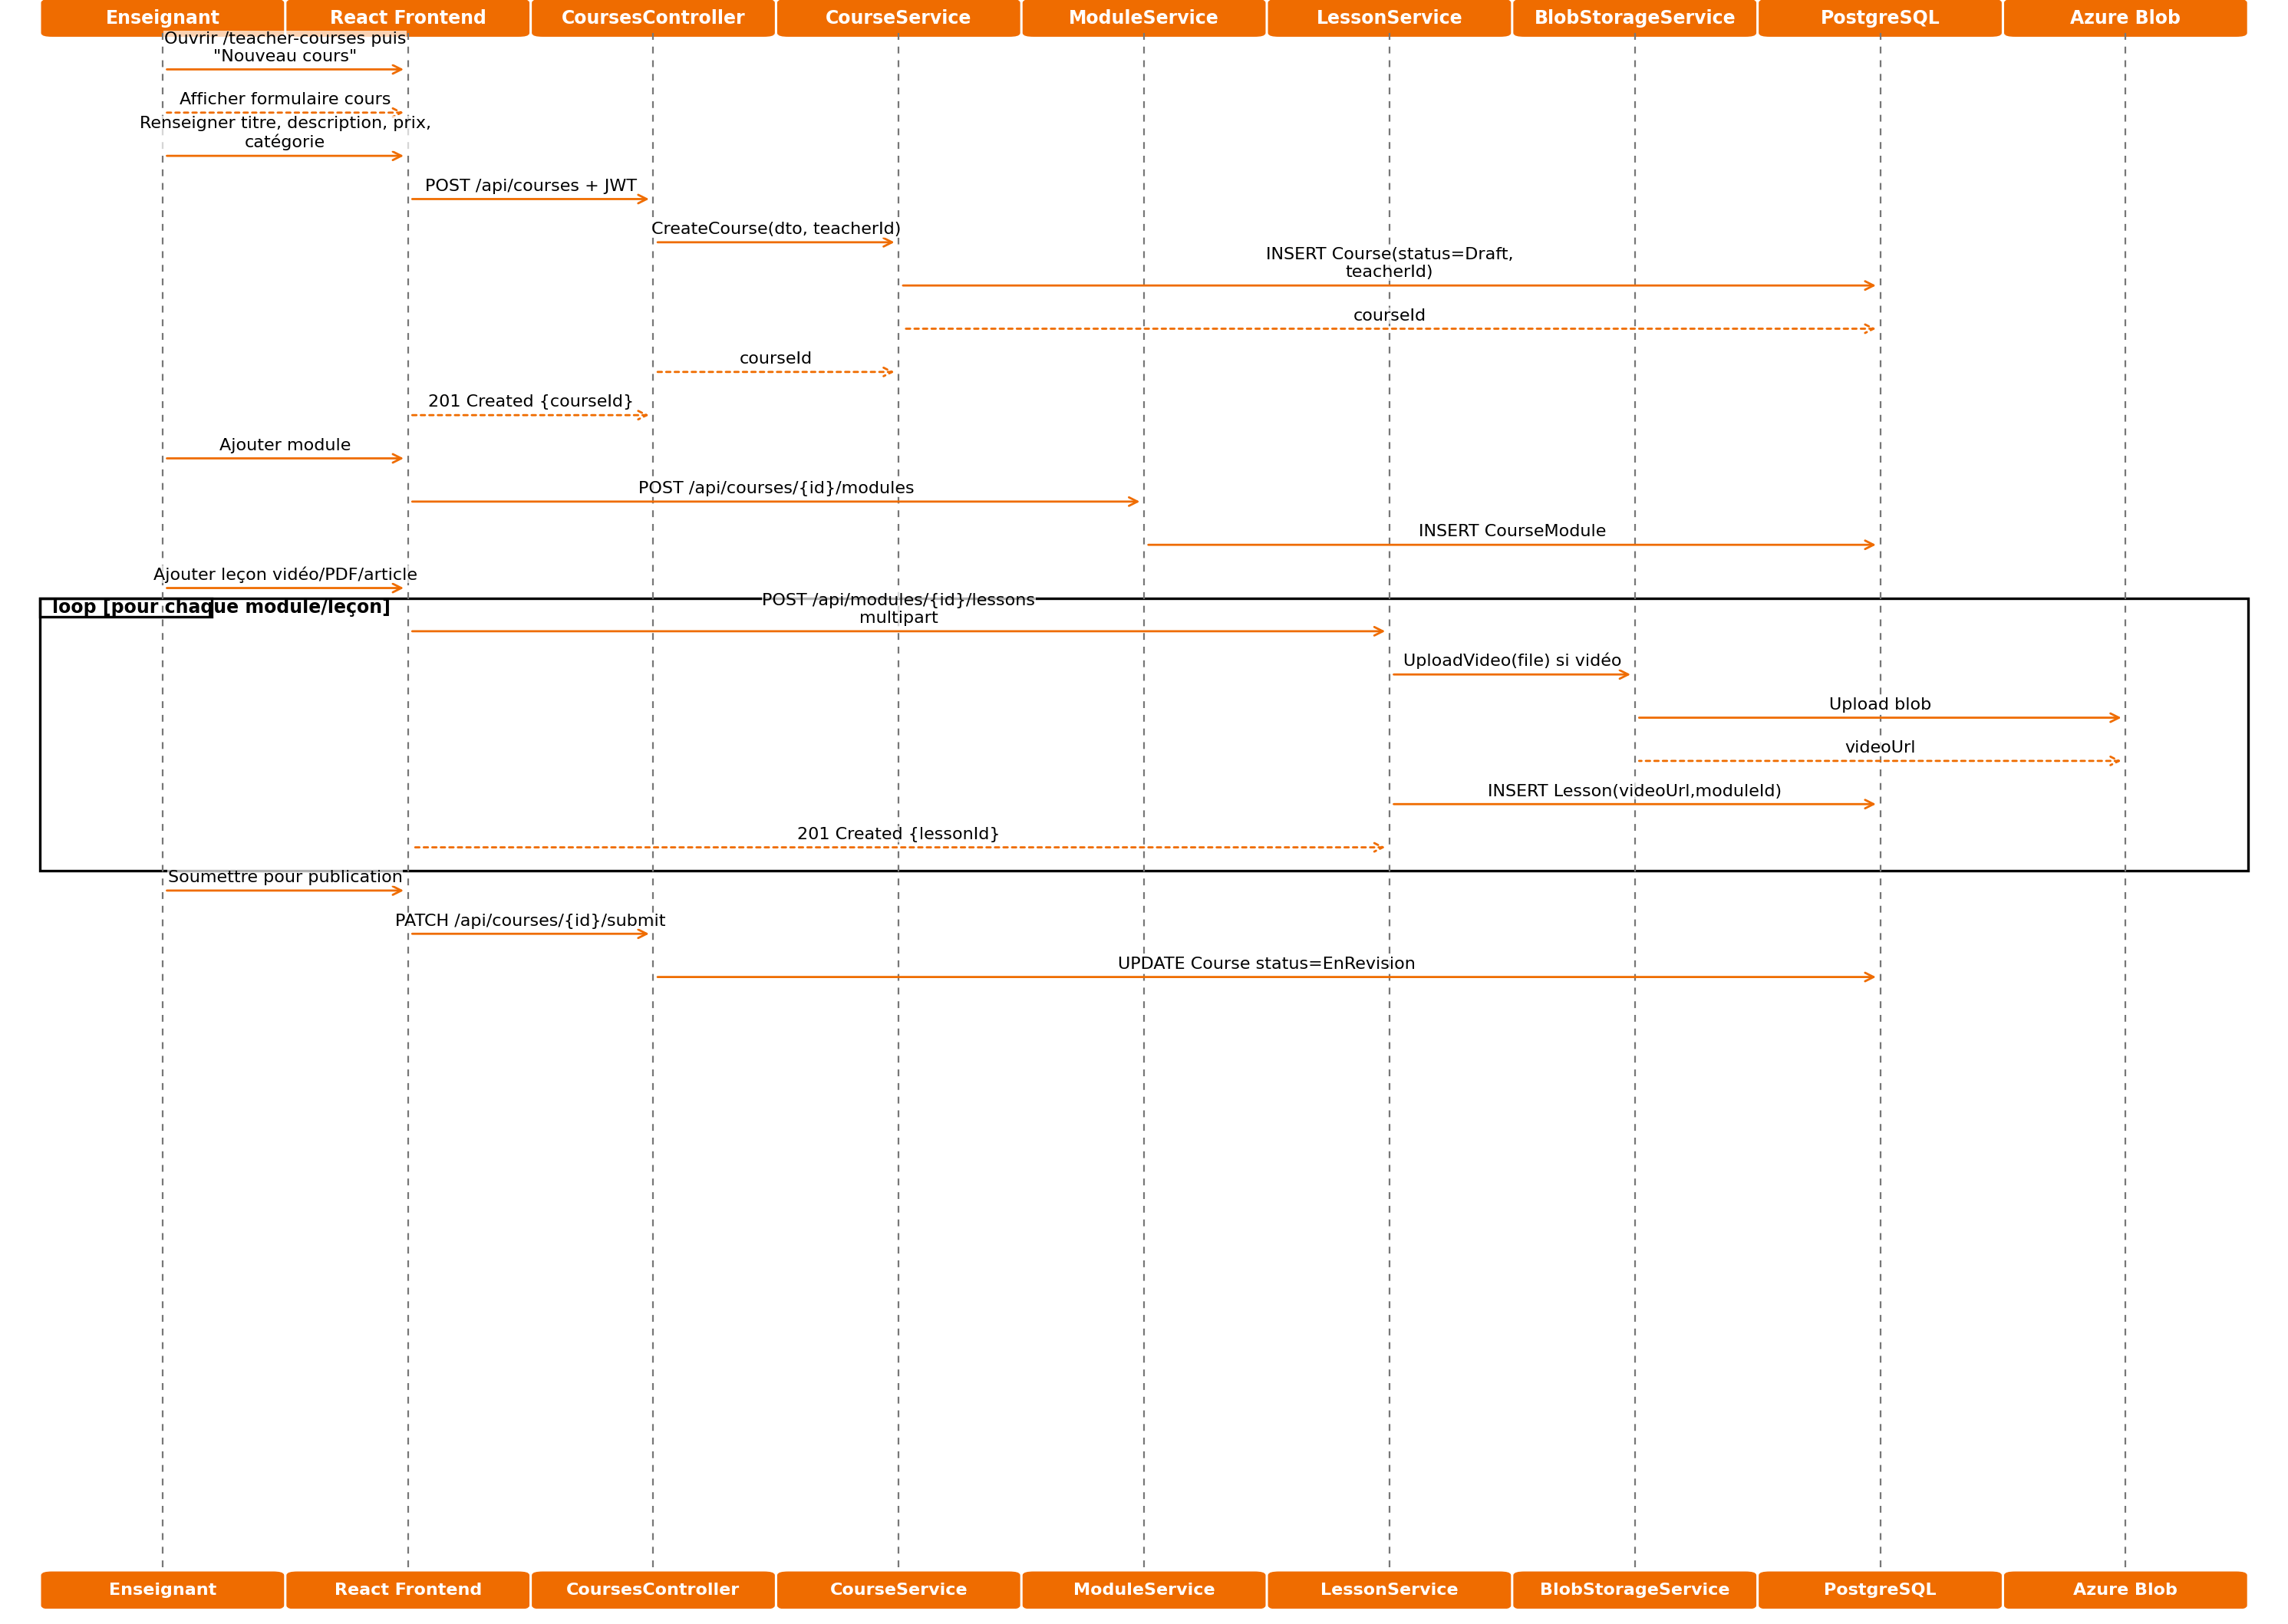
\includegraphics[width=\textwidth]{DIAGRAMME_DE_SEQUENCE_-_CREATION_DE_COURS__ENSEIGNANT_.png}
  \caption{Diagramme de séquence – Création de cours par l'enseignant}
  \label{fig:seq_cours}
\end{figure}
\noindent  Ce diagramme modélise le processus de création de contenu pédagogique dans EduBoard par un enseignant, depuis la création d’un cours jusqu’à sa publication.

\medskip

\noindent Il décrit les principales opérations de gestion du contenu, incluant l’ajout de modules, de leçons et de quiz, ainsi que l’upload de fichiers multimédias vers Azure Blob Storage. Chaque étape est sécurisée par un contrôle de propriété garantissant que seul l’enseignant propriétaire peut modifier son contenu.
% ------------------------------------------------------------
\section{Diagramme de Classes}

\begin{figure}[H] \centering 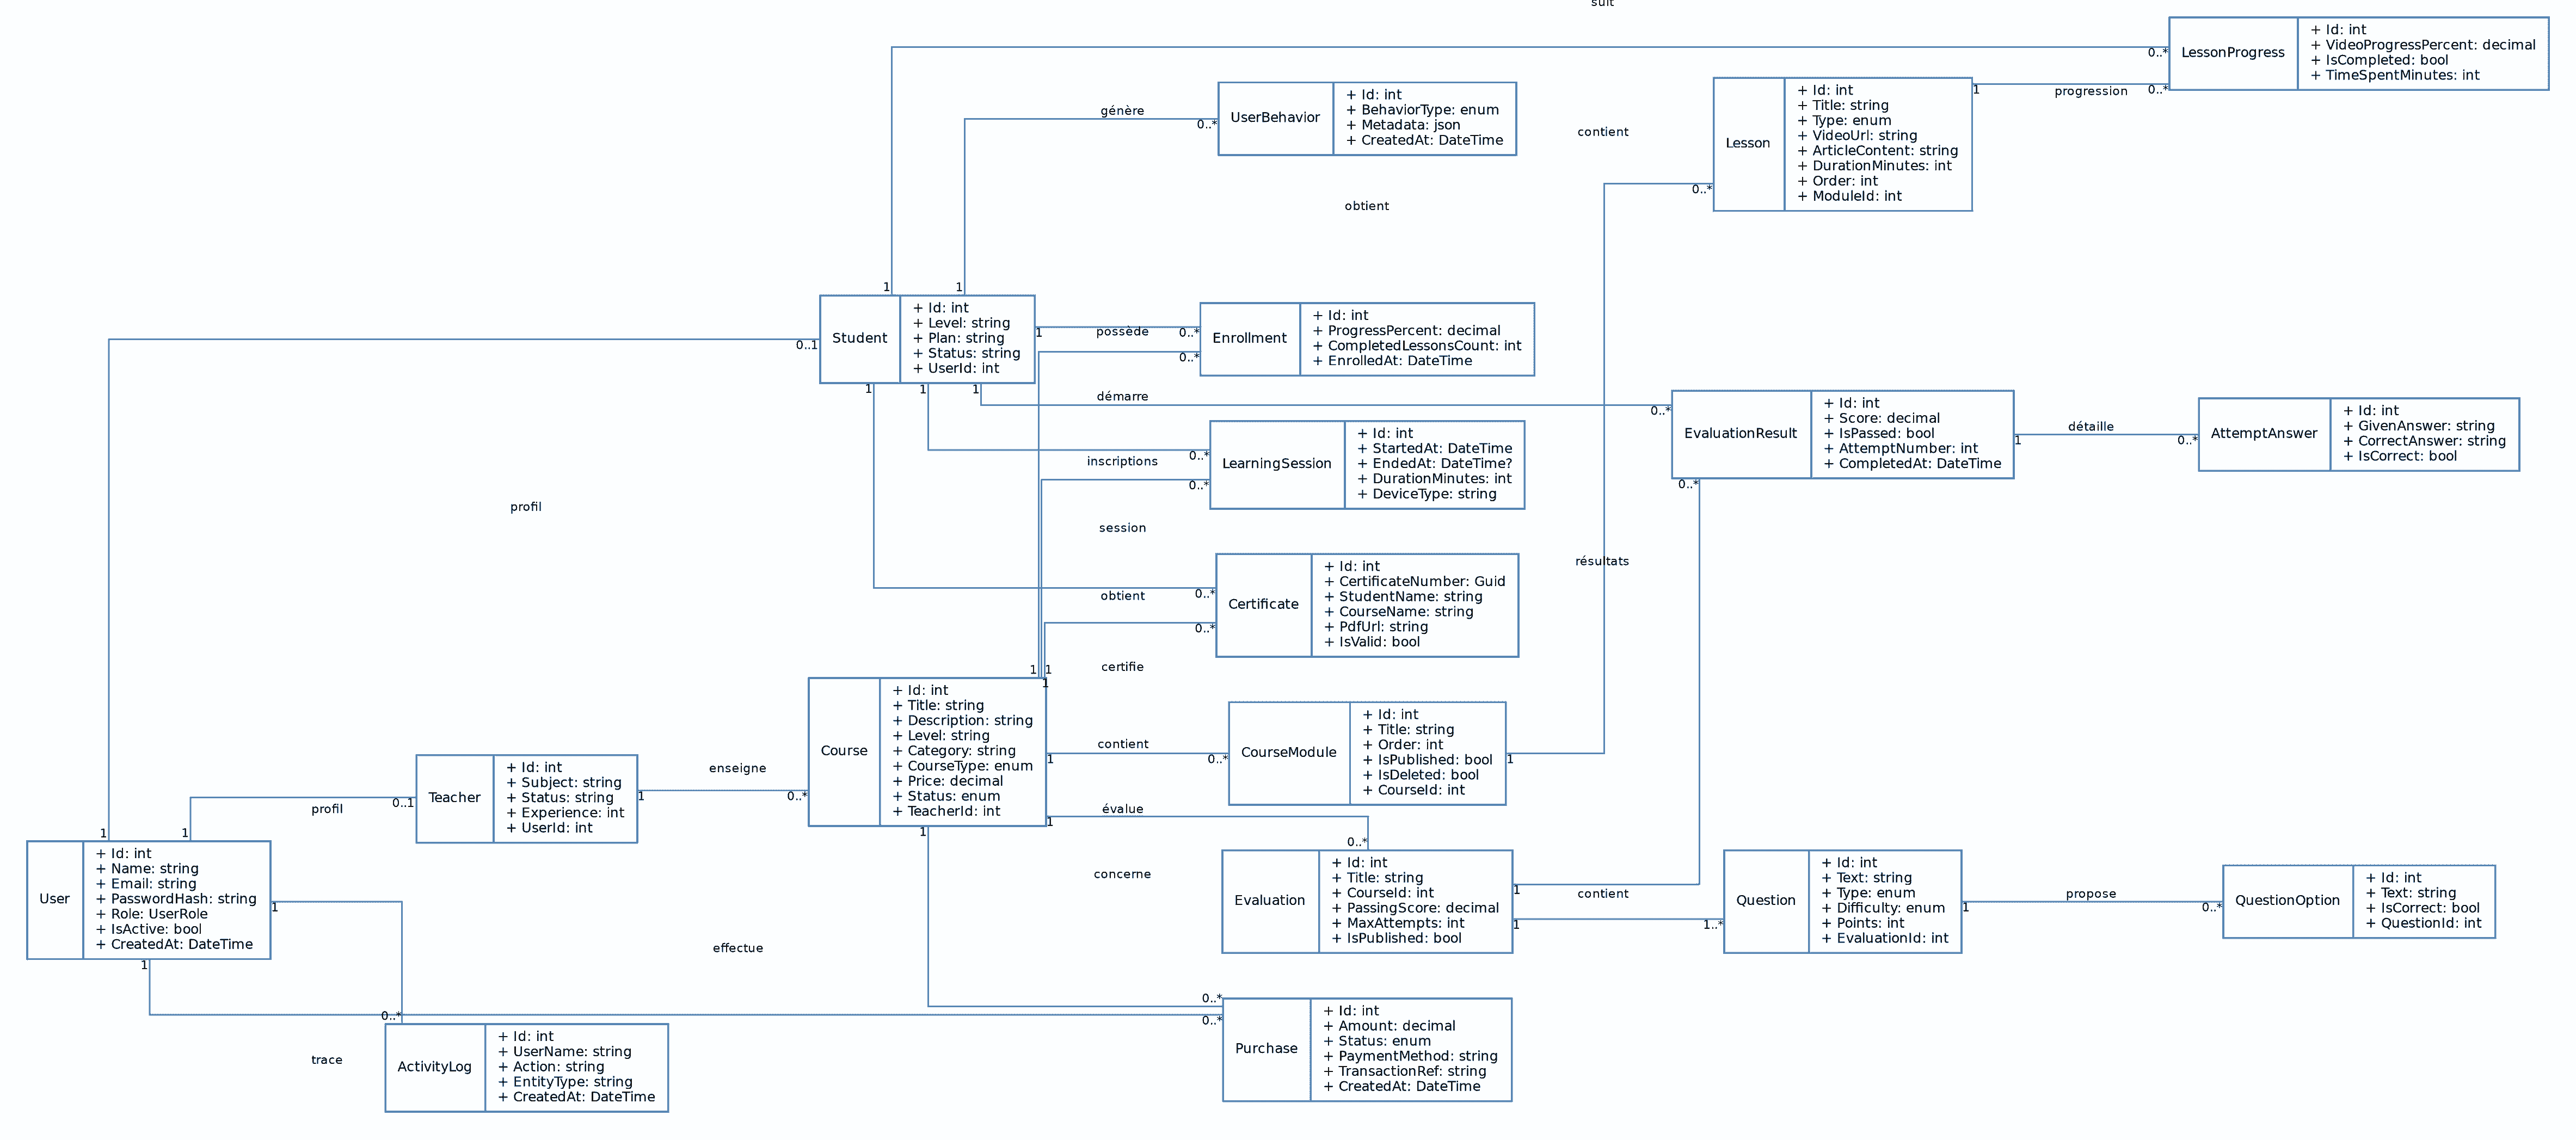
\includegraphics[width=\textwidth]{DIAGRAMME_DE_CLASSES__MODELE_DOMAINE_.png} \caption{Diagramme de classes – Modèle domaine EduBoard} \label{fig:classes} 
\end{figure}

\begin{table}[H]
  \centering
  \caption{Description des entités du modèle domaine}
  \label{tab:entites}
  \begin{tabularx}{\textwidth}{llX}
    \toprule
    \textbf{Entité} & \textbf{Table SQL} & \textbf{Attributs clés} \\
    \midrule
    User         & Users         & Id, Name, Email, PasswordHash, Role, IsActive \\
    Course       & Courses       & Id, Title, Price, OriginalPrice, ThumbnailUrl, Rating, TeacherId \\
    Module       & Modules       & Id, Title, Order, CourseId \\
    Lesson       & Lessons       & Id, Title, Content, VideoUrl, Order, ModuleId \\
    Quiz         & Quizzes       & Id, Title, CourseId, IsPlacement, TimeLimit \\
    Question     & Questions     & Id, Text, Type, Points, QuizId \\
    Answer       & Answers       & Id, Text, IsCorrect, QuestionId \\
    Purchase     & Purchases     & Id, UserId, CourseId, Amount, Status, TransactionRef \\
    QuizAttempt  & QuizAttempts  & Id, UserId, QuizId, Score, AIFeedback, CompletedAt \\
    Certificate  & Certificates  & Id, UserId, CourseId, PdfUrl, IssuedAt \\
    UserProgress & UserProgress  & Id, UserId, CourseId, CompletedLessons, ProgressPercent \\
    \bottomrule
  \end{tabularx}
\end{table}

% ------------------------------------------------------------
\section{Diagramme de Déploiement}

\begin{figure}[H]
  \centering
  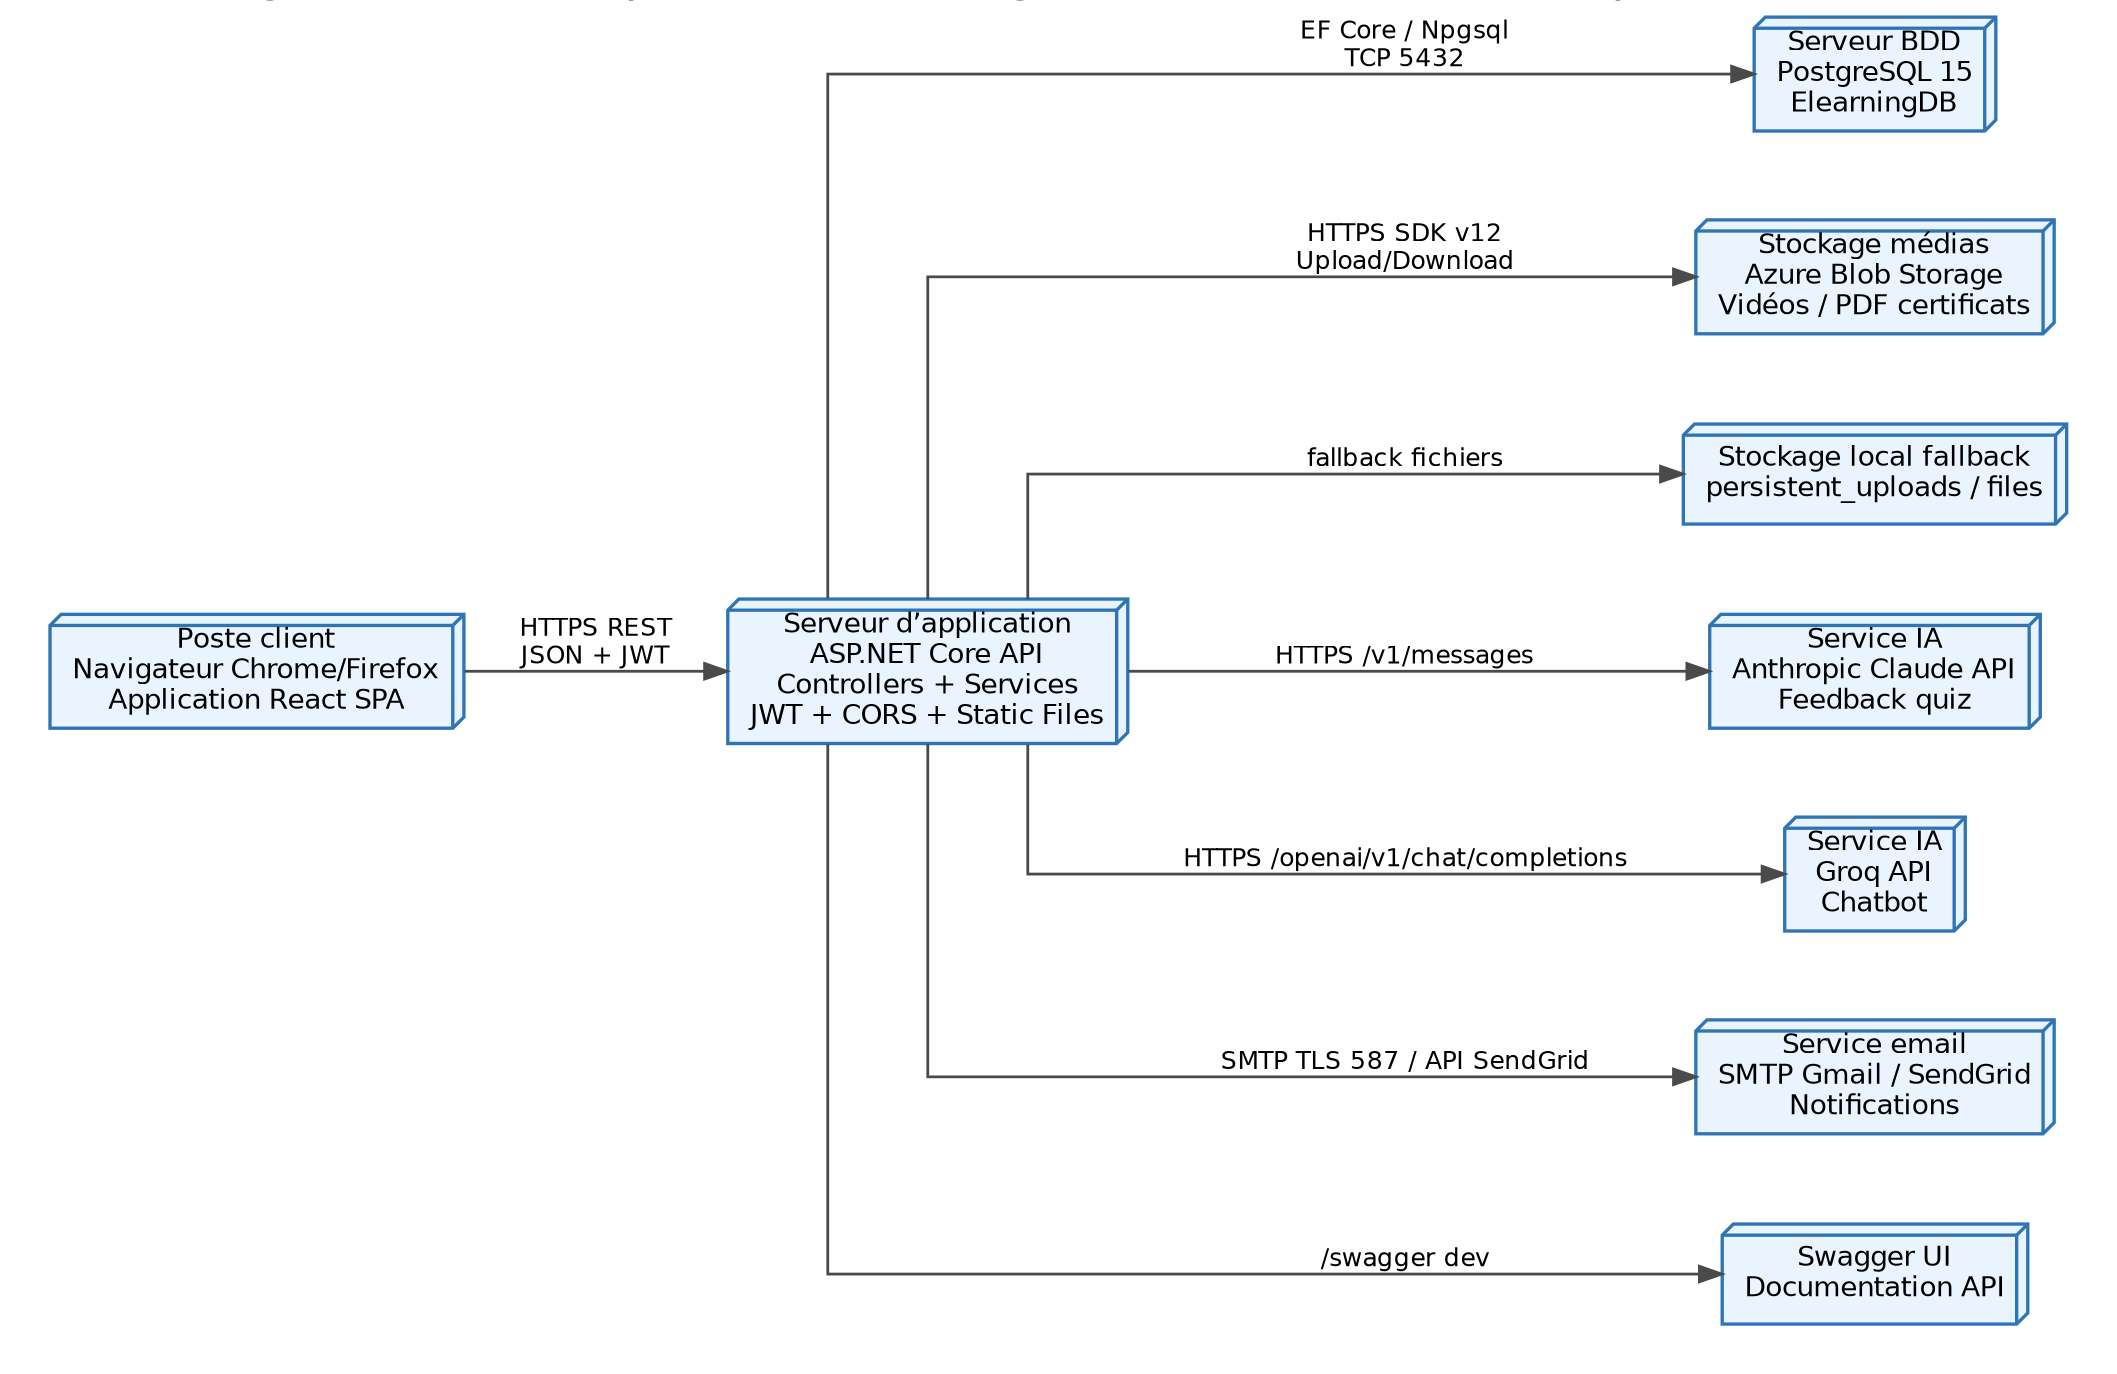
\includegraphics[width=\textwidth]{DIAGRAMME_DE_DEPLOIEMENT.png}
  \caption{Diagramme de déploiement – Architecture technique EduBoard}
  \label{fig:deploiement}
\end{figure}

L'architecture de déploiement comprend quatre nœuds principaux~:
\begin{itemize}
  \item \textbf{Poste Client~:} Navigateur web exécutant l'application React.js (port 3000).
  \item \textbf{Serveur d'Application~:} ASP.NET Core 8 (port 5132) avec middleware JWT,
        CORS et fichiers statiques.
  \item \textbf{Serveur BDD~:} PostgreSQL 15 (port 5432) avec ElearningDB.
  \item \textbf{Services Cloud \& IA~:} Azure Blob Storage, API Anthropic, API Groq, SMTP Gmail.
\end{itemize}

% ------------------------------------------------------------
\section{Diagrammes d'États-Transitions}

\subsection{Cycle de Vie d'un Cours}

\begin{figure}[H]
  \centering
  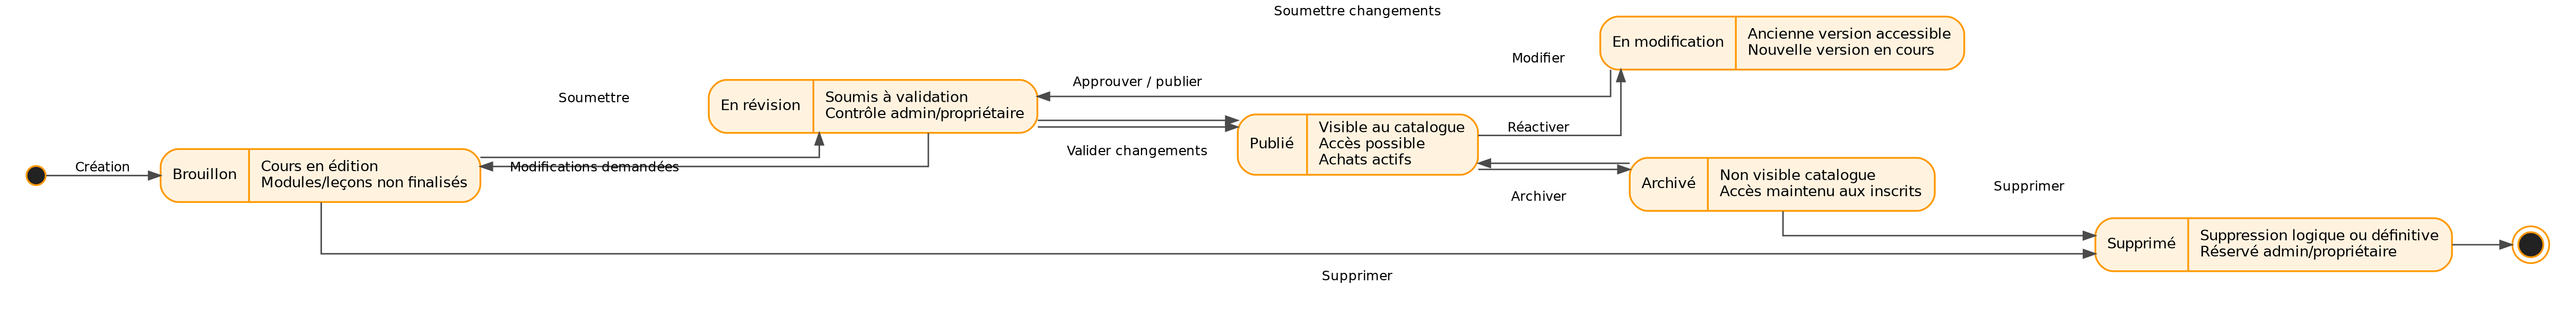
\includegraphics[width=0.85\textwidth]{DIAGRAMME_D_ETATS-TRANSITIONS_-_CYCLE_DE_VIE_D_UN_Cours.png}
  \caption{Diagramme d'états-transitions – Cycle de vie d'un cours}
  \label{fig:etat_cours}
\end{figure}

\section*{Cycle de vie d’un cours (EduBoard)}

Le diagramme décrit les états de maturité d’un cours pédagogique dans la plateforme EduBoard, ainsi que les transitions entre ces états et leur impact sur la visibilité dans le catalogue.

\subsection*{États du cours}
\begin{itemize}
    \item \textbf{Brouillon} : cours en cours de création, non visible par les étudiants.
    \item \textbf{En Révision} : cours soumis à validation par un administrateur.
    \item \textbf{Publié} : cours accessible aux étudiants et visible dans le catalogue.
    \item \textbf{En Mise à Jour} : cours temporairement retiré du catalogue pour modification par l’enseignant.
    \item \textbf{Archivé} : cours retiré définitivement du catalogue, mais toujours accessible aux étudiants déjà inscrits.
\end{itemize}

\subsection*{Règles de visibilité}
Seuls les cours ayant l’état \textbf{Publié} sont accessibles via l’API \texttt{GET /api/courses} sans authentification.  
Les cours \textbf{Archivés} restent consultables par les étudiants déjà inscrits via leur tableau de bord, assurant la continuité pédagogique.

\subsection*{Objectif}
Ce modèle permet de structurer le processus éditorial, de définir clairement les responsabilités des acteurs à chaque transition, et de garantir une publication contrôlée ainsi qu’une modération efficace.

\subsection{Cycle de Vie d'un Achat}

\begin{figure}[H]
  \centering
  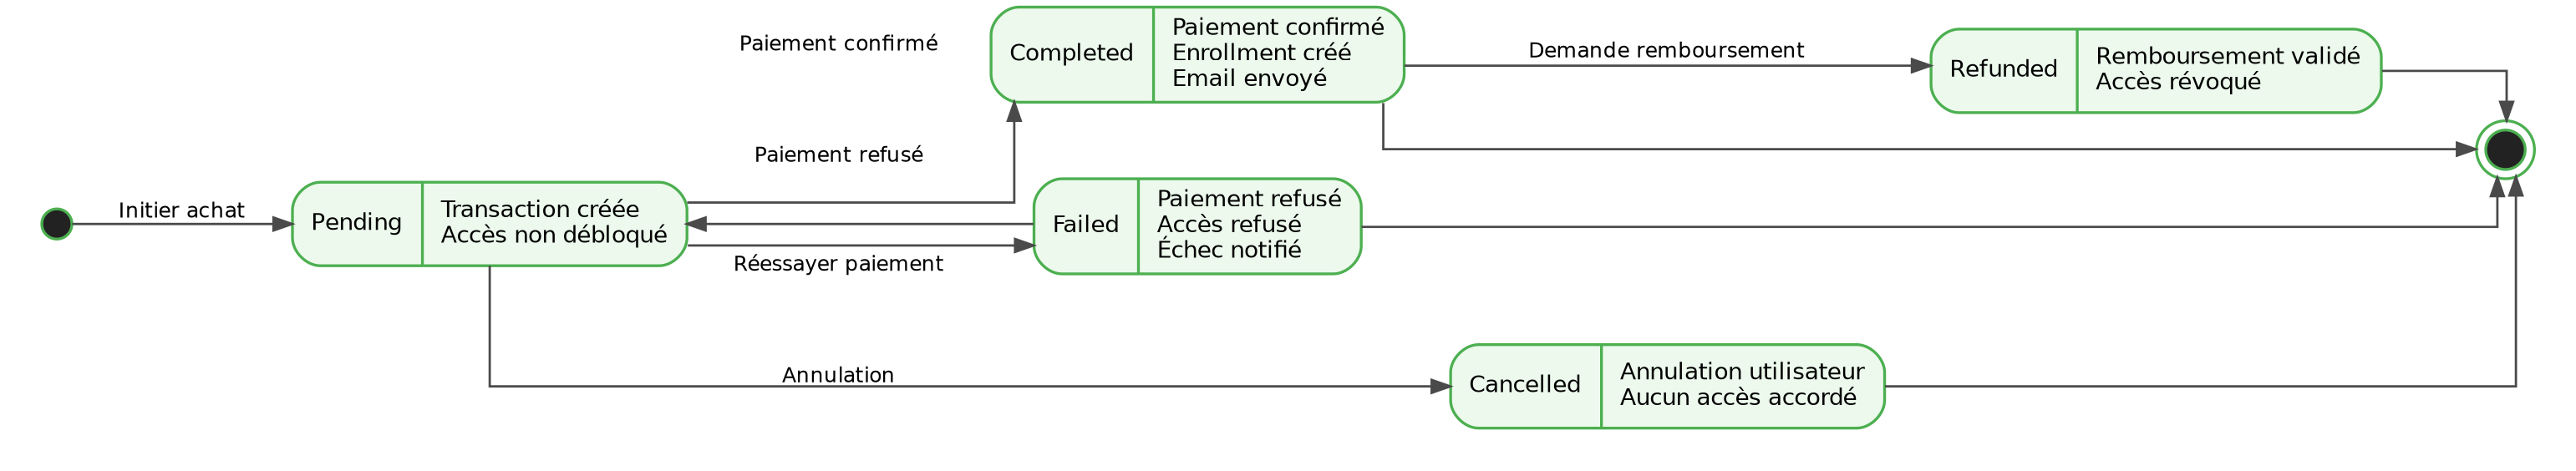
\includegraphics[width=0.85\textwidth]{DIAGRAMME_D_ETATS-TRANSITIONS_-_CYCLE_DE_VIE_D_UN_ACHAT.png}
  \caption{Diagramme d'états-transitions – Cycle de vie d'un achat}
  \label{fig:etat_achat}
\end{figure}

\section*{Cycle de vie d’une transaction (Purchase - EduBoard)}

Ce diagramme modélise les états successifs d’une entité \textit{Purchase} dans EduBoard, depuis son initiation jusqu’à sa finalisation. Il permet de garantir l’intégrité transactionnelle et la cohérence entre le paiement et les droits d’accès des étudiants.

\subsection*{États de la transaction}
\begin{itemize}
    \item \textbf{Pending} : état initial lors de l’initiation du paiement.
    \item \textbf{Completed} : paiement validé par la passerelle (Flouci), déclenchant l’accès au cours.
    \item \textbf{Failed} : paiement refusé par la passerelle de paiement.
    \item \textbf{Cancelled} : transaction annulée par l’utilisateur avant validation.
    \item \textbf{Refunded} : remboursement effectué par l’administrateur, entraînant la révocation de l’accès.
\end{itemize}

\subsection*{Règle métier}
L’inscription (\textit{Enrollment}) n’est créée qu’après une transition vers l’état \textbf{Completed}.  
Une transition de \textbf{Completed} vers \textbf{Refunded} entraîne la suppression ou la désactivation de l’inscription associée.

\subsection*{Objectif}
Ce modèle vise à prévenir les incohérences entre paiement et accès aux cours, notamment l’accès sans paiement confirmé, les doublons de paiement ou le maintien d’accès après remboursement.

% ------------------------------------------------------------
\section{Architecture Frontend React.js}

\subsection{Structure de l'Application}

\begin{table}[H]
  \centering
  \caption{Structure et routes de l'application React EduBoard}
  \label{tab:routes}
  \begin{tabularx}{\textwidth}{llX}
    \toprule
    \textbf{Catégorie} & \textbf{Route} & \textbf{Composant / Description} \\
    \midrule
    Public      & \texttt{/}                    & LandingPage \\
                & \texttt{/login}               & Login \\
                & \texttt{/register}            & Register \\
    Admin       & \texttt{/dashboard}           & AdminDashboard \\
    Enseignant  & \texttt{/teacher-dashboard}   & TeacherDashboard \\
                & \texttt{/teacher-courses}     & CoursesList \\
    Étudiant    & \texttt{/student-dashboard}   & StudentDashboard \\
                & \texttt{/quiz/:id}            & QuizDetails \\
                & \texttt{/certificates}        & CertificatesPage \\
    Paiement    & \texttt{/courses/:id/purchase}& CoursePurchasePage \\
                & \texttt{/payment/success}     & PaymentSuccessPage \\
    \bottomrule
  \end{tabularx}
\end{table}

\subsection{Architecture des Services Backend}

\begin{table}[H]
  \centering
  \caption{Services backend et leurs responsabilités}
  \label{tab:services}
  \begin{tabularx}{\textwidth}{llX}
    \toprule
    \textbf{Service} & \textbf{Interface} & \textbf{Responsabilité} \\
    \midrule
    EvaluationService       & IEvaluationService       & Correction quiz, calcul score \\
    QuizFeedbackService     & IQuizFeedbackService     & Appel API Anthropic, feedback pédagogique \\
    ChatbotService          & –                        & Appel API Groq, conversation \\
    RecommendationService   & IRecommendationService   & Recommandations personnalisées \\
    ProgressService         & IProgressService         & Suivi progression par cours \\
    CertificateService      & ICertificateService      & Génération PDF (QuestPDF) \\
    VideoService            & IVideoService            & Upload vidéo Azure Blob \\
    BlobStorageService      & IBlobStorageService      & Opérations Azure Blob \\
    EmailService            & –                        & Envoi emails SMTP Gmail \\
    BehaviorService         & IBehaviorService         & Analyse comportement étudiant \\
    \bottomrule
  \end{tabularx}
\end{table}

\section*{Conclusion}
\addcontentsline{toc}{section}{Conclusion}

Ce chapitre a présenté l'architecture globale d'EduBoard, les choix technologiques
justifiés, les diagrammes \ac{UML} complets et la conception des services. Le chapitre
suivant présente la réalisation concrète, les interfaces et les tests effectués.

% ============================================================
%  09_chapitre4_realisation.tex  –  Chapitre 4 : Réalisation et Tests
% ============================================================
\chapter{Réalisation et Tests}

\section*{Introduction}
\addcontentsline{toc}{section}{Introduction}

Ce chapitre présente l'environnement de développement, les interfaces réalisées pour
chaque rôle, les fonctionnalités implémentées et les tests effectués pour valider la
solution EduBoard.

% ------------------------------------------------------------
\section{Environnement de Travail}

\subsection{Environnement Matériel}

Le développement de la plateforme EduBoard a été réalisé sur une machine de
développement aux caractéristiques techniques suivantes, permettant de faire tourner
simultanément le frontend React.js, le backend ASP.NET Core 8, la base de données
PostgreSQL ainsi que les outils de développement associés.

\begin{table}[H]
  \centering
  \caption{Spécifications matérielles du poste de développement}
  \label{tab:materiel}
  \renewcommand{\arraystretch}{1.3}
  \begin{tabularx}{\textwidth}{|l|X|}
    \hline
    \textbf{Composant} & \textbf{Spécification} \\
    \hline
    Processeur           & Intel Core i9-13900H 13\textsuperscript{e} gén.\ (2,60\,GHz, 24 cœurs) \\
    \hline
    Mémoire RAM          & 16\,GB DDR5 \\
    \hline
    Carte graphique      & Intel Iris Xe Graphics \\
    \hline
    Stockage             & SSD NVMe 477\,GB \\
    \hline
    Système d'exploitation & Windows 11 Famille (Version 25H2, 64 bits) \\
    \hline
    Résolution écran     & 1920 $\times$ 1080 pixels \\
    \hline
  \end{tabularx}
\end{table}


\subsection{Environnement Logiciel}

Le développement d’EduBoard repose sur un ensemble cohérent d’outils et de technologies couvrant le développement, la gestion de versions, la base de données, la documentation et les services cloud. Ces choix technologiques assurent la performance, la maintenabilité et la compatibilité de la plateforme.


\section{Technologies Utilisées}
% ------------------------------------------------------------
le tableau présente les principales technologies rretenus pour le développement de la plateforme EduBoard , ainsi que leurs roles respectifs au seins de l'architecture.

\begin{table}[H]
  \centering
  \caption{Outils logiciels et environnements de développement}
  \label{tab:logiciels}
  \renewcommand{\arraystretch}{1.35}
  \begin{tabularx}{\textwidth}{|l|l|X|}
    \hline
    \textbf{Outil} & \textbf{Version} & \textbf{Rôle dans le projet} \\
    \hline
    Visual Studio Code     & 1.90+     & Éditeur pour le frontend React.js avec
                                         extensions TypeScript, ESLint, Prettier
                                         et GitLens. \\
    \hline
    React.js                & 18    & Développement de l’interface utilisateur avec React, gestion des dépendances à l’aide de npm et utilisation de Vite comme outil de développement et de génération des builds.. \\
    \hline
    .NET               & 8.0       & Framework backend pour le développement
                                         de l'\ac{API} \ac{REST} ASP.NET Core,
                                         compilation et publication. \\
    \hline
    PostgreSQL             & 15        & Système de gestion de \ac{BDD} relationnelle
                                         pour la persistance des données EduBoard. \\
    \hline
    pgAdmin 4              & 7.x       & Interface graphique d'administration et de
                                         requêtage PostgreSQL. \\
    \hline
    Git / GitHub           & --        & Gestion de versions avec GitFlow (branches
                                         feature, pull requests, historique du code). \\
    \hline
    Swagger / OpenAPI      & 3.0       & Documentation interactive de l'\ac{API}
                                         \ac{REST}, accessible via \texttt{/swagger}. \\
   
                                         
    \hline
    PlantUML               & --        & Génération des diagrammes \ac{UML} du
                                         système (activité, séquence, classes). \\
    \hline
  \end{tabularx}
\end{table}
\section{Language de développement}

\noindent\textbf{Figma :}
est un outil de conception graphique vectoriel. Figma a été déployé en amont
du code pour concevoir le design global de l'application. Il a permis
de créer les maquettes haute fidélité.

\begin{figure}[H]
\centering
\includegraphics[width=0.2\textwidth]{figures/images/figma (1).png}
\caption{Logo Figma}
\label{fig:figma}
\end{figure}

  %\item \includegraphics[height=0.8cm]{images/vscode.png}
  \textbf{Visual Studio Code (1.90+)} : éditeur utilisé pour le développement du frontend React.js avec support TypeScript et extensions dédiées.

  %\item \includegraphics[height=0.8cm]{images/nodejs.png}
  \textbf{Node.js (20 LTS)} : environnement d’exécution JavaScript utilisé pour le frontend et la gestion des dépendances npm.

  %\item \includegraphics[height=0.8cm]{images/postgresql.png}
  \textbf{PostgreSQL (15)} : système de gestion de base de données relationnelle utilisé pour stocker les données de la plateforme.

  %\item \includegraphics[height=0.8cm]{images/pgadmin.png}
  \textbf{pgAdmin 4 (7.x)} : outil d’administration graphique de la base de données PostgreSQL.

  %\item \includegraphics[height=0.8cm]{images/github.png}
  \textbf{Git / GitHub} : gestion de versions et collaboration via GitFlow (branches, pull requests, suivi du code).

  %\item \includegraphics[height=0.8cm]{images/dotnet.png}
  \textbf{.NET SDK (8.0)} : framework backend utilisé pour le développement de l’API REST ASP.NET Core.

  %\item \includegraphics[height=0.8cm]{images/swagger.png}
  \textbf{Swagger / OpenAPI (3.0)} : outil de documentation et de test interactif des API REST.

  %\item \includegraphics[height=0.8cm]{images/plantuml.png}
  \textbf{PlantUML} : outil de modélisation UML utilisé pour générer les diagrammes du système.

  %\item \includegraphics[height=0.8cm]{images/docker.png}
  \textbf{Docker} : conteneurisation des services pour assurer un déploiement reproductible.
\end{itemize}
% ------------------------------------------------------------
\subsection{Page d'Accueil (Landing Page)}

\begin{figure}[H]
  \centering
  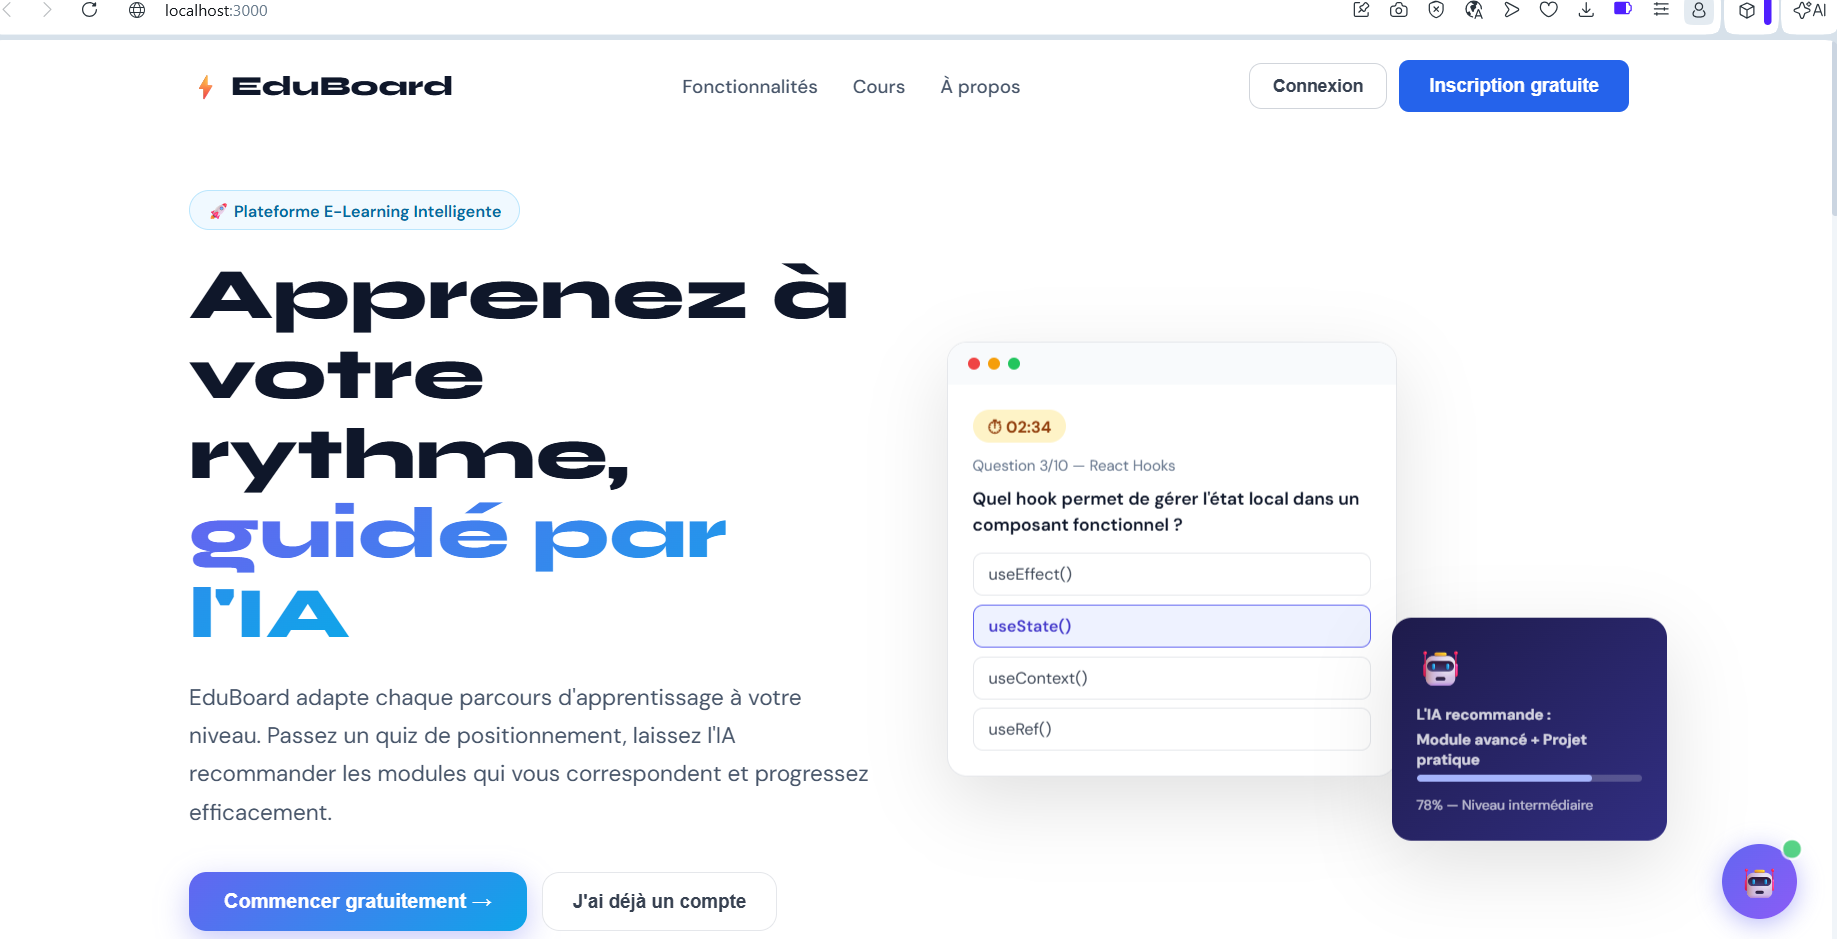
\includegraphics[width=\textwidth]{capture_landing.png}
  \caption{Page d'accueil de la plateforme EduBoard (Landing Page)}
  \label{fig:landing}
\end{figure}

\vspace{1cm}

\subsection{Authentification – Connexion et Inscription}

\begin{figure}[H]
  \centering

  % -------- Login --------
  \begin{subfigure}[b]{0.95\textwidth}
    \centering
    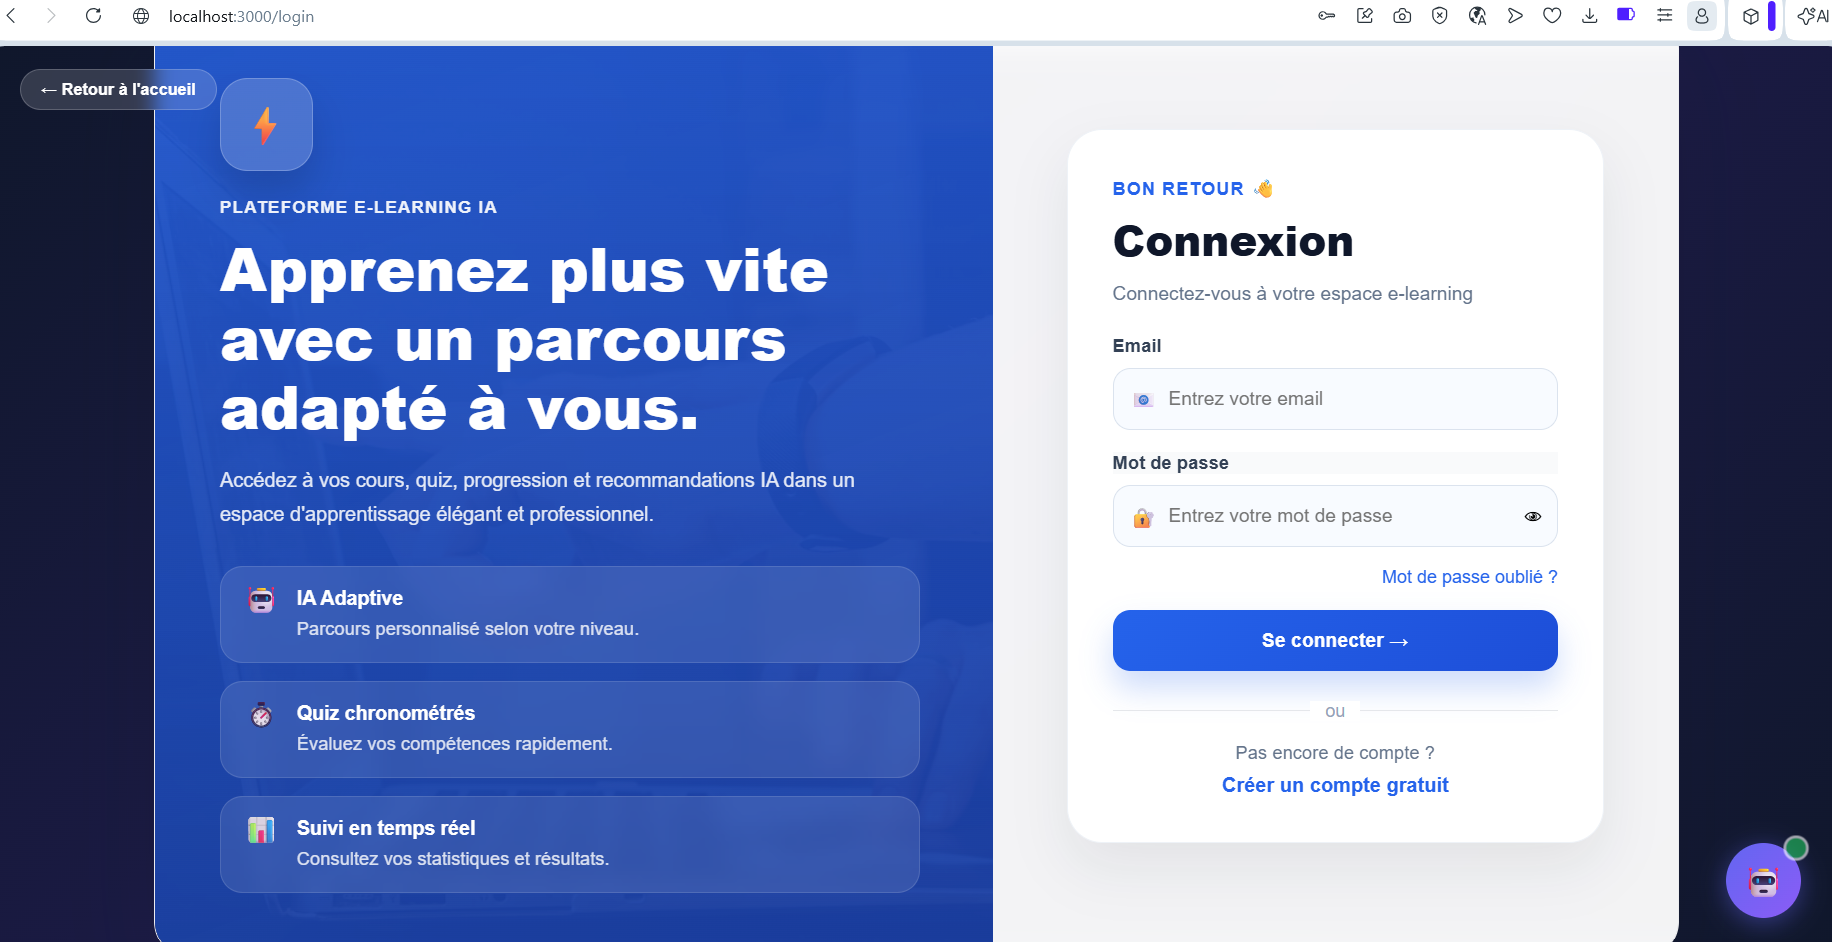
\includegraphics[width=0.95\textwidth]{capture_login.png}
    \caption{Page de connexion}
  \end{subfigure}
  \hfill

  % -------- Register --------
  \begin{subfigure}[b]{0.95\textwidth}
    \centering
    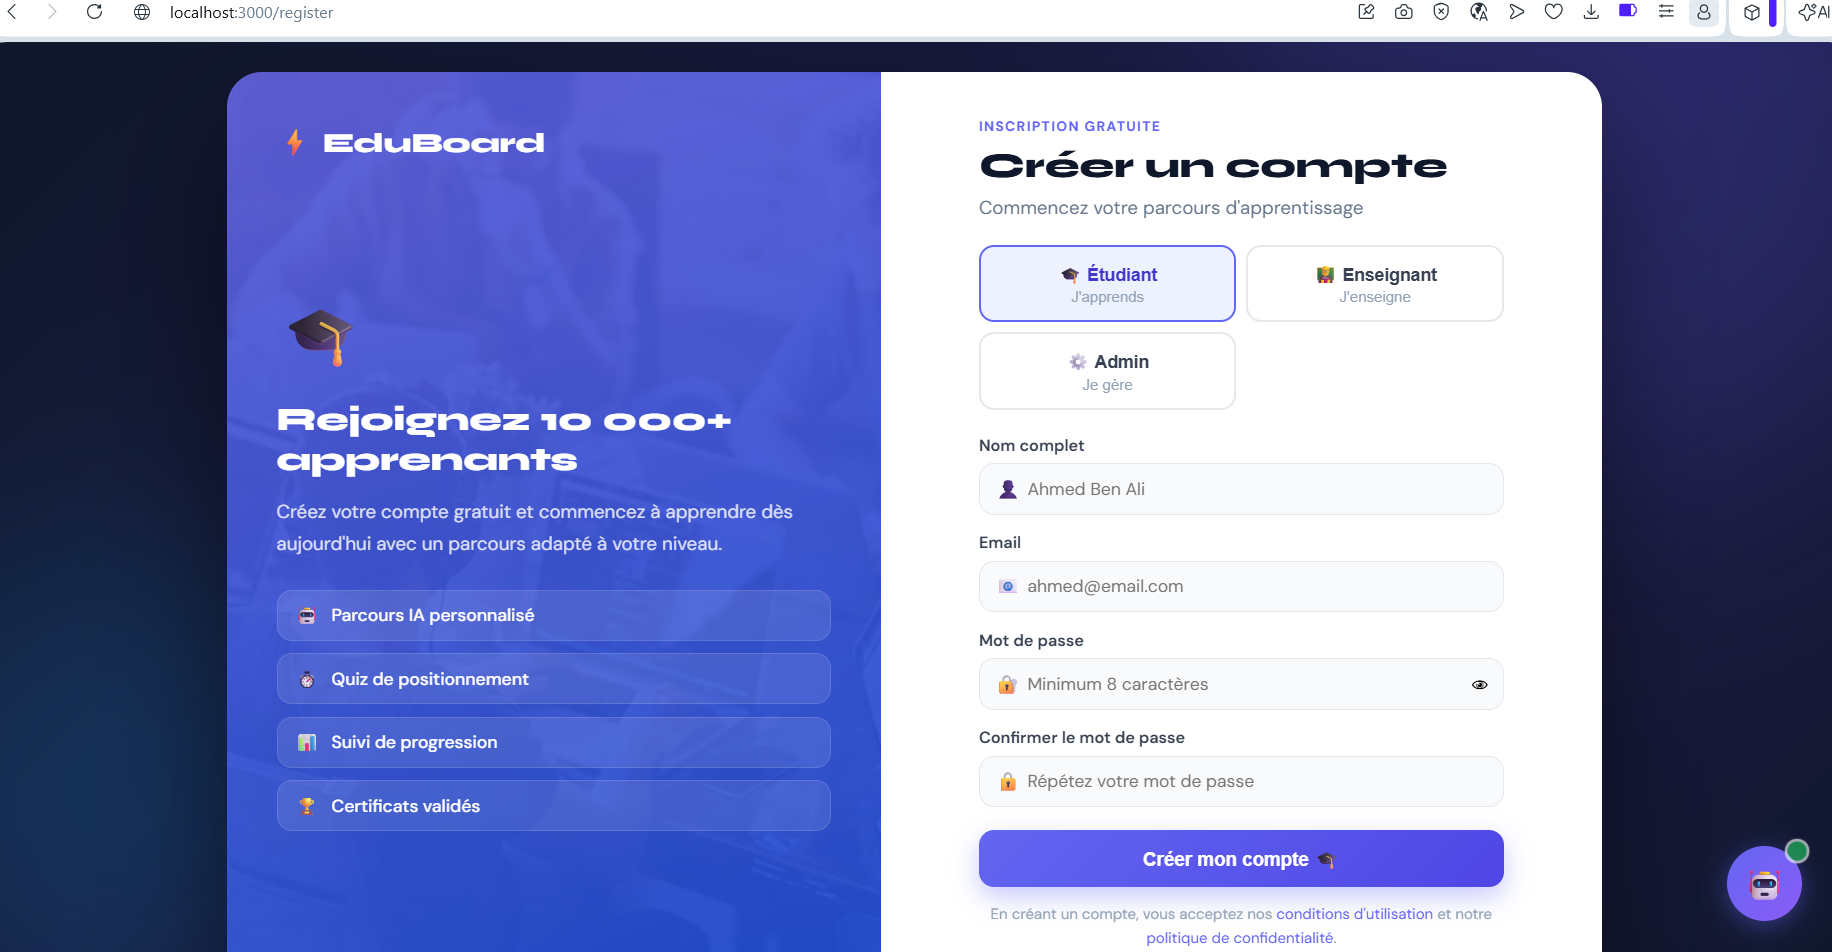
\includegraphics[width=0.95\textwidth]{capture_register.png}
    \caption{Page d'inscription}
  \end{subfigure}

  \caption{Interfaces d'authentification de la plateforme EduBoard}
  \label{fig:auth}
\end{figure}

\subsection{Tableau de Bord Étudiant}

\begin{figure}[H]
  \centering

  % -------- Image 1 --------
  \begin{subfigure}[b]{0.95\textwidth}
    \centering
    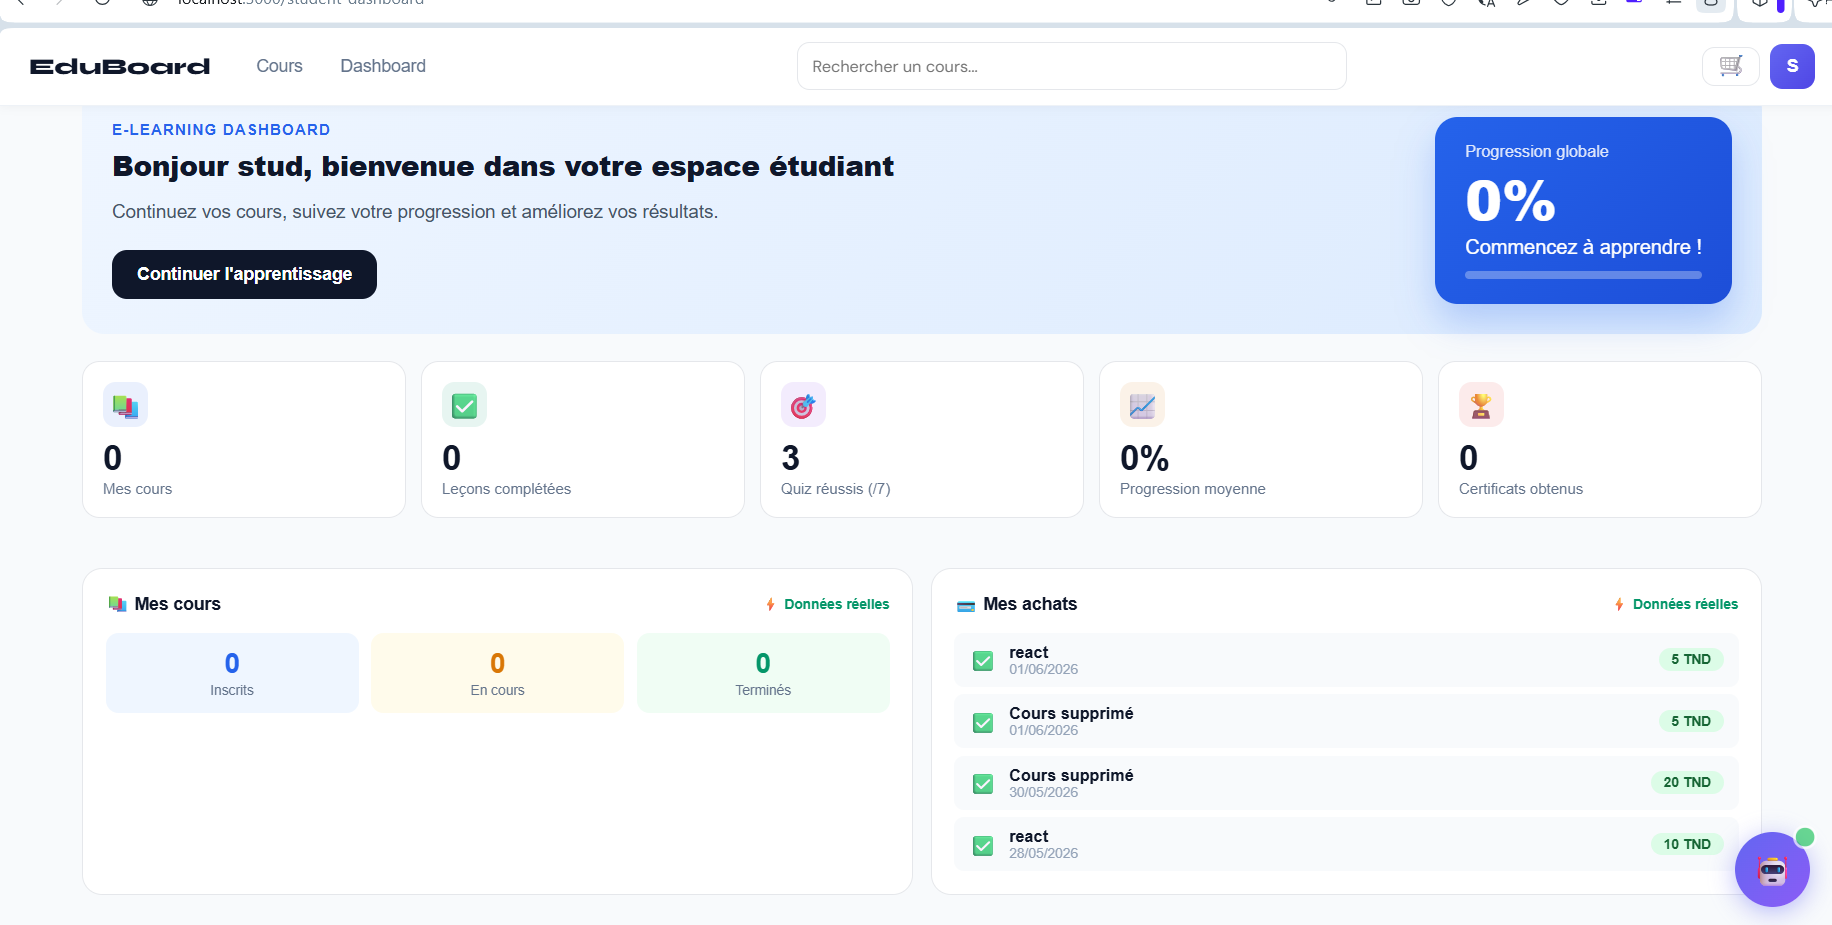
\includegraphics[width=0.95\textwidth]{capture_student_dashboard.png}
    \caption{Dashboard étudiant – vue principale}
  \end{subfigure}

  \vspace{0.8cm}

  % -------- Image 2 --------
  \begin{subfigure}[b]{0.95\textwidth}
    \centering
    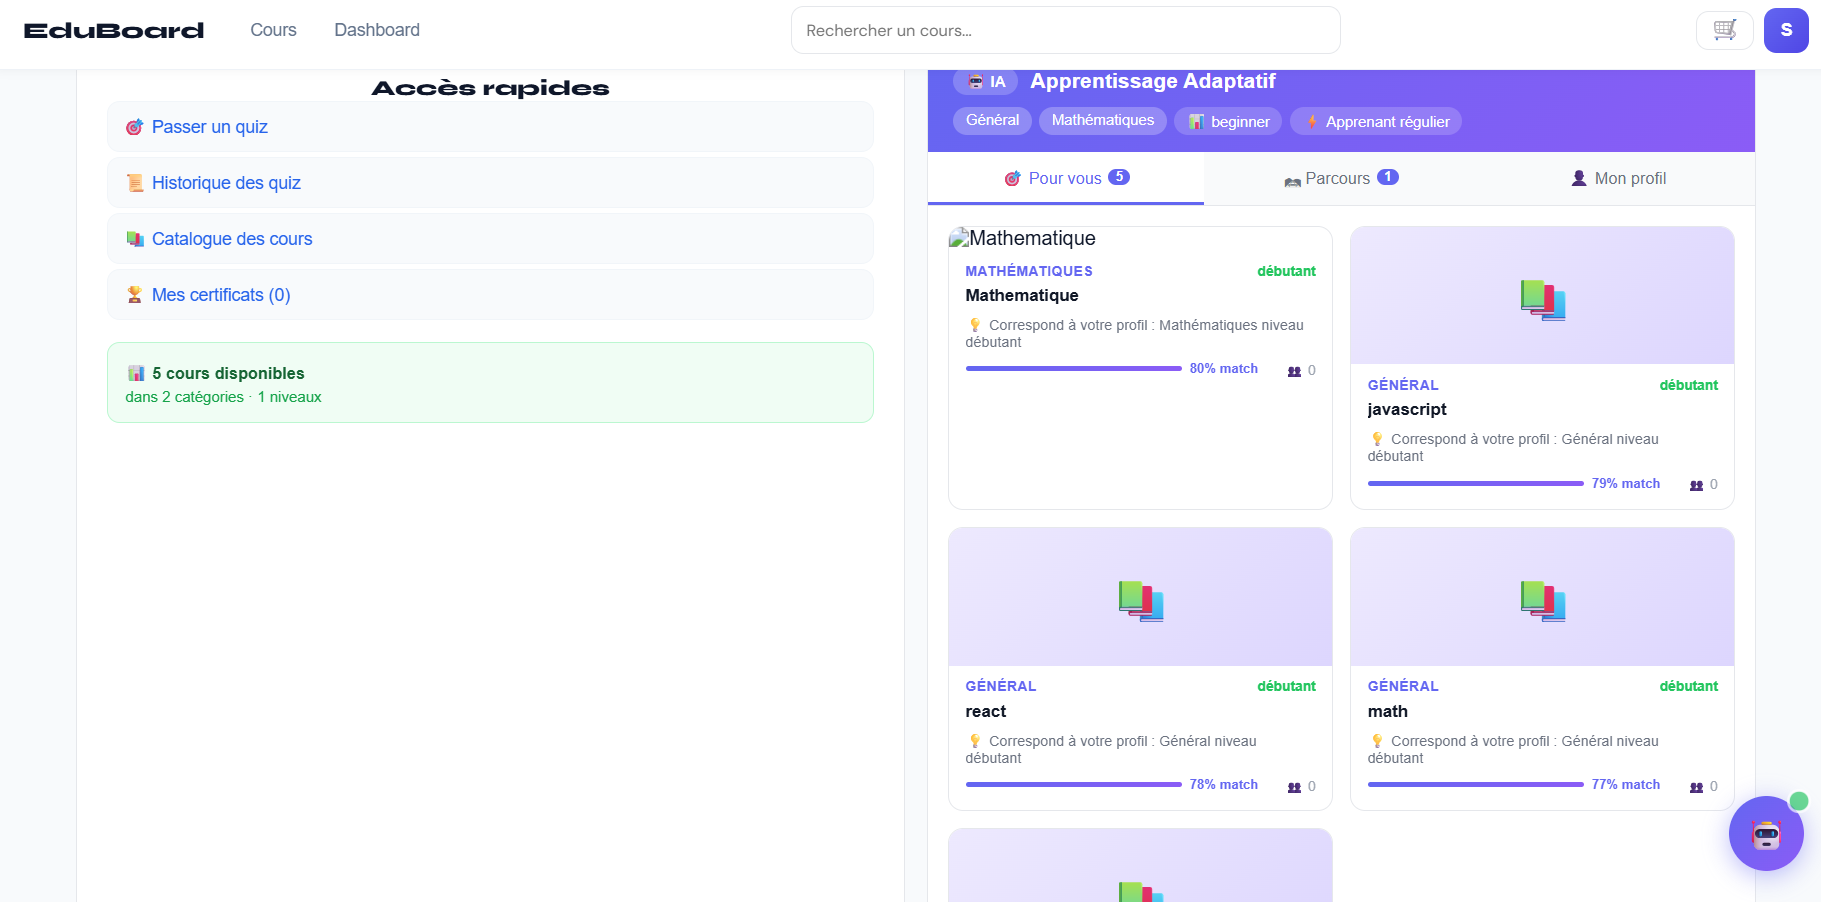
\includegraphics[width=0.95\textwidth]{capture_student_dashboard2.png}
    \caption{Dashboard étudiant – vue secondaire}
  \end{subfigure}

  \caption{Tableau de bord étudiant (\texttt{/student-dashboard})}
  \label{fig:dashboard_etudiant}
\end{figure}

\subsection{Tableau de Bord Enseignant}

\begin{figure}[H]
  \centering
  \begin{subfigure}[b]{0.48\textwidth}
    \includegraphics[width=\textwidth]{interfaceteacher1.png}
    \caption{Dashboard enseignant – vue 1}
  \end{subfigure}
  \hfill
  \begin{subfigure}[b]{0.48\textwidth}
    \includegraphics[width=\textwidth]{interfaceteacher2.png}
    \caption{Dashboard enseignant – vue 2}
  \end{subfigure}
  \caption{Tableau de bord Enseignant (\texttt{/teacher-dashboard})}
  \label{fig:dashboard_enseignant}
\end{figure}

\subsection{Tableau de Bord Administrateur}

\begin{figure}[H]
  \centering
  \includegraphics[width=\textwidth]{capture_admin_dashboard.png}
  \caption{Tableau de bord Administrateur (\texttt{/dashboard})}
  \label{fig:dashboard_admin}
\end{figure}

\subsection{Catalogue et Détail de Cours}

\begin{figure}[H]
  \centering
  \begin{subfigure}[b]{0.48\textwidth}
    \includegraphics[width=\textwidth]{capture_courses_list.png}
    \caption{Catalogue des cours}
  \end{subfigure}
  \hfill
  \begin{subfigure}[b]{0.48\textwidth}
    \includegraphics[width=\textwidth]{capture_course_detail.png}
    \caption{Détail d'un cours}
  \end{subfigure}
  \caption{Interfaces de gestion des cours}
  \label{fig:cours}
\end{figure}

\subsection{Interface de Passage de Quiz avec Feedback IA}

\begin{figure}[H]
  \centering
  \begin{subfigure}[b]{0.48\textwidth}
    \includegraphics[width=\textwidth]{capture_quiz_passage.png}
    \caption{Passage du quiz}
  \end{subfigure}
  \hfill
  \begin{subfigure}[b]{0.48\textwidth}
    \includegraphics[width=\textwidth]{capture_quiz_result.png}
    \caption{Résultats et feedback IA}
  \end{subfigure}
  \caption{Interface de quiz avec feedback IA (Anthropic Claude)}
  \label{fig:quiz}
\end{figure}

\subsection{Chatbot Pédagogique IA}

\begin{figure}[H]
  \centering
  \includegraphics[width=0.5\textwidth]{capture_chatbot.png}
  \caption{ChatbotWidget – Assistant pédagogique IA (Groq)}
  \label{fig:chatbot}
\end{figure}

\subsection{Processus de Paiement}

\begin{figure}[H]
  \centering
  \begin{subfigure}[b]{0.48\textwidth}
    \includegraphics[width=\textwidth]{capture_payment.png}
    \caption{Page de paiement}
  \end{subfigure}
  \hfill
  \begin{subfigure}[b]{0.48\textwidth}
    \includegraphics[width=\textwidth]{capture_payment_success.png}
    \caption{Page de succès paiement}
  \end{subfigure}
  \caption{Interfaces du processus de paiement}
  \label{fig:paiement}
\end{figure}

\subsection{Certificats}

\begin{figure}[H]
  \centering
  \includegraphics[width=\textwidth]{capture_certificates.png}
  \caption{Page des certificats (\texttt{/certificates}) avec téléchargement PDF}
  \label{fig:certificats}
\end{figure}

% ------------------------------------------------------------
\section{Tests}

\subsection{Tests Fonctionnels}

\begin{table}[H]
  \centering
  \caption{Résultats des tests fonctionnels principaux}
  \label{tab:tests}
  \begin{tabularx}{\textwidth}{lllc}
    \toprule
    \textbf{Scénario testé} & \textbf{Endpoint} & \textbf{Résultat attendu} & \textbf{Statut} \\
    \midrule
    Inscription utilisateur     & POST \texttt{/api/auth/register}     & 201 Created         & \checkmark \\
    Connexion valide            & POST \texttt{/api/auth/login}         & 200 + JWT           & \checkmark \\
    Connexion invalide          & POST \texttt{/api/auth/login}         & 401                 & \checkmark \\
    Création cours              & POST \texttt{/api/courses}            & 201 Created         & \checkmark \\
    Upload vidéo                & POST \texttt{/api/lessons}            & 201 + URL           & \checkmark \\
    Passage quiz                & POST \texttt{/api/quizzes/submit}     & 200 + score         & \checkmark \\
    Feedback IA Anthropic       & Via QuizFeedbackService               & Texte feedback      & \checkmark \\
    Achat cours (succès)        & POST \texttt{/api/purchases}          & 200 Completed       & \checkmark \\
    Achat cours (échec)         & POST \texttt{/api/purchases}          & 400 Failed          & \checkmark \\
    Génération certificat PDF   & Via CertificateService                & PDF généré          & \checkmark \\
    Chatbot réponse             & POST \texttt{/api/chatbot/message}    & 200 + réponse       & \checkmark \\
    Recommandations             & GET \texttt{/api/recommendations}     & 200 + liste         & \checkmark \\
    \bottomrule
  \end{tabularx}
\end{table}

\subsection{Tests de Sécurité}

\begin{itemize}
  \item \textbf{Protection des routes~:} toutes les routes protégées retournent 401
        Unauthorized sans token JWT valide.
  \item \textbf{Autorisation par rôle~:} les routes réservées retournent 403 Forbidden
        avec un rôle inadéquat.
  \item \textbf{CORS~:} les origines non listées dans la politique AllowReactDev sont
        bien rejetées.
  \item \textbf{Hashage BCrypt~:} les mots de passe sont hashés en BDD et jamais
        stockés en clair.
  \item \textbf{Expiration JWT~:} le token expiré est correctement rejeté
        (\texttt{ClockSkew = TimeSpan.Zero}).
\end{itemize}

\subsection{Tests de Performance}

Des tests de charge basiques ont été effectués avec Postman Collections Runner pour
simuler des accès concurrents. Les endpoints d'authentification et de consultation de
cours maintiennent un temps de réponse inférieur à 500 ms pour 50 requêtes
simultanées, satisfaisant ainsi l'exigence non fonctionnelle de performance définie
au chapitre~2.

\section*{Conclusion}
\addcontentsline{toc}{section}{Conclusion}

Ce chapitre a présenté l'implémentation complète d'EduBoard~: environnement de
développement, interfaces utilisateurs pour chaque rôle et résultats des tests. La
plateforme répond à l'ensemble des besoins identifiés au chapitre~2 et constitue une
solution innovante, robuste et scalable.

% ============================================================
%  10_conclusion_generale.tex  –  Conclusion Générale
% ============================================================
\chapter*{Conclusion Générale}
\addcontentsline{toc}{chapter}{Conclusion Générale}
\markboth{Conclusion Générale}{Conclusion Générale}

Ce projet de fin d'études nous a permis de concevoir, développer et valider
\textbf{EduBoard}, une plateforme e-learning intelligente de nouvelle génération
intégrant les dernières avancées en intelligence artificielle générative. Réalisé au
sein de Whitecape Technologies sur une période de quatre mois (Février – Mai 2026),
ce projet représente une expérience professionnelle authentique et complète, depuis la
phase d'analyse et de spécification jusqu'à la livraison d'une solution opérationnelle,
testée et documentée.

\medskip

Sur le plan fonctionnel, EduBoard répond à une problématique réelle et croissante du
marché de la formation en ligne~: la personnalisation de l'expérience d'apprentissage.
En intégrant nativement l'API Claude d'Anthropic pour le feedback pédagogique
contextuel et l'API Groq pour le chatbot 24h/24, la plateforme se distingue
fondamentalement des solutions traditionnelles.

\medskip

Sur le plan technique, ce projet a permis d'approfondir et de mettre en pratique~:
\begin{itemize}
  \item Architecture full-stack moderne avec ASP.NET Core 8 et React.js 18.
  \item Conception orientée services avec respect des principes SOLID.
  \item Gestion de base de données relationnelle avec PostgreSQL 15 et EF Core.
  \item Authentification et autorisation sécurisées avec JWT et RBAC.
  \item Intégration d'APIs d'\ac{IA} générative (Anthropic Claude, Groq).
  \item Génération de documents PDF avec QuestPDF.
  \item Gestion du cycle de vie complet avec la méthodologie Scrum.
\end{itemize}

\medskip

\textbf{Perspectives d'évolution~:}
\begin{itemize}
  \item Application mobile (React Native ou Flutter) pour un accès hors ligne.
  \item Déploiement cloud sur Azure ou AWS en mode SaaS, avec scaling horizontal.
  \item Gamification (badges, points XP, classements) pour augmenter l'engagement.
  \item Forum et collaboration entre étudiants (discussions par cours).
  \item Analytics avancés avec Business Intelligence (export CSV/Excel).
  \item Multi-langue avec internationalisation complète (i18n).
  \item Tests automatisés unitaires et d'intégration avec xUnit et Jest/Cypress.
  \item Modération \ac{IA} du contenu.
\end{itemize}

\medskip

En définitive, ce projet constitue bien plus qu'un exercice académique~: c'est une
solution logicielle réelle, fonctionnelle et commercialisable, aboutissement de cinq
années de formation à l'ESPITA.


% ---- Bibliographie ----
% ============================================================
%  11_bibliographie.tex  –  Bibliographie et Webographie
% ============================================================
\chapter*{Bibliographie et Webographie}
\addcontentsline{toc}{chapter}{Bibliographie et Webographie}
\markboth{Bibliographie et Webographie}{Bibliographie et Webographie}

\section*{Documentation Technique Officielle}

\begin{itemize}
  \item Microsoft. \textit{ASP.NET Core 8 Documentation}.
        \url{https://docs.microsoft.com/aspnet/core}
  \item Anthropic. \textit{Claude API Documentation}.
        \url{https://docs.anthropic.com}
  \item Groq. \textit{Groq API Documentation}.
        \url{https://console.groq.com/docs}
  \item PostgreSQL Global Development Group. \textit{PostgreSQL 15 Documentation}.
        \url{https://www.postgresql.org/docs/15/}
  \item React Development Team. \textit{React 18 Documentation}.
        \url{https://react.dev}
  \item Microsoft. \textit{Entity Framework Core 8 Documentation}.
        \url{https://learn.microsoft.com/ef/core}
  \item QuestPDF Team. \textit{QuestPDF Documentation}.
        \url{https://www.questpdf.com/documentation}
  \item Microsoft Azure. \textit{Azure Blob Storage Documentation}.
        \url{https://docs.microsoft.com/azure/storage/blobs}
\end{itemize}

\section*{Ouvrages de Référence}

\begin{itemize}
  \item Fowler, M. (2018). \textit{Patterns of Enterprise Application Architecture}.
        Addison-Wesley.
  \item Freeman, A. (2022). \textit{Pro ASP.NET Core 6}. Apress.
  \item Wieruch, R. (2022). \textit{The Road to React}. Self-published.
  \item Schwaber, K. \& Sutherland, J. (2020). \textit{The Scrum Guide}.
        \url{https://www.scrum.org}
\end{itemize}

\section*{Sites Web}

\begin{itemize}
  \item Whitecape Technologies. \url{https://www.whitecapetech.com}
  \item JSON Web Tokens. \url{https://jwt.io}
  \item PlantUML. \url{https://plantuml.com}
  \item Swagger / OpenAPI. \url{https://swagger.io}
  \item Stack Overflow. \url{https://stackoverflow.com}
\end{itemize}


% ---- Annexes ----
\appendix
% ============================================================
%  12_annexes.tex  –  Annexes
% ============================================================

% ---- Annexe A : Extrait Program.cs ----
\chapter{Extrait du Code Source – Program.cs}
\label{ann:program_cs}

\begin{lstlisting}[language={[Sharp]C}, caption={Configuration de l'injection de dépendances (Program.cs)}, label={lst:program}]
// Dependency Injection
builder.Services.AddHttpClient<IAIGradingService, AIGradingService>();
builder.Services.AddHttpClient<ChatbotService>();

// QuizFeedbackService avec header Anthropic
builder.Services.AddHttpClient<IQuizFeedbackService, QuizFeedbackService>(
    client =>
    {
        client.DefaultRequestHeaders.Add("x-api-key",
            builder.Configuration["Anthropic:ApiKey"] ?? "");
        client.DefaultRequestHeaders.Add(
            "anthropic-version", "2023-06-01");
    });

builder.Services.AddScoped<IEvaluationService, EvaluationService>();
builder.Services.AddScoped<IProgressService, ProgressService>();
builder.Services.AddScoped<ICertificateService, CertificateService>();
builder.Services.AddScoped<IVideoService, VideoService>();
builder.Services.AddScoped<IBlobStorageService, BlobStorageService>();
\end{lstlisting}

% ---- Annexe B : Migration SQL ----
\chapter{Migration SQL – Table Purchases}
\label{ann:sql_purchases}

\begin{lstlisting}[language=SQL, caption={Migration SQL de création de la table Purchases}, label={lst:sql_purchases}]
CREATE TABLE IF NOT EXISTS Purchases (
    Id              SERIAL PRIMARY KEY,
    UserId          INT NOT NULL,
    CourseId        INT NOT NULL,
    Amount          DECIMAL(10,2) NOT NULL,
    Status          VARCHAR(50) DEFAULT 'Pending',
    PaymentMethod   VARCHAR(50),
    TransactionRef  VARCHAR(255),
    CreatedAt       TIMESTAMP DEFAULT CURRENT_TIMESTAMP
);

-- Enrichissement de la table Courses
ALTER TABLE Courses ADD COLUMN IF NOT EXISTS
    Price           DECIMAL(10,2) DEFAULT 0;
ALTER TABLE Courses ADD COLUMN IF NOT EXISTS
    OriginalPrice   DECIMAL(10,2) DEFAULT 0;
ALTER TABLE Courses ADD COLUMN IF NOT EXISTS
    ThumbnailUrl    TEXT;
ALTER TABLE Courses ADD COLUMN IF NOT EXISTS
    TotalHours      INT DEFAULT 0;
ALTER TABLE Courses ADD COLUMN IF NOT EXISTS
    Rating          DECIMAL(3,2) DEFAULT 0;
\end{lstlisting}

% ---- Annexe C : Guide d'insertion des captures ----
\chapter{Guide d'Insertion des Captures d'Écran}
\label{ann:guide_images}

\begin{center}
\textbf{Structure recommandée du dossier \texttt{figures/images/}}
\end{center}
\begin{table}[H]
\centering
\caption{Correspondance fichiers images – contenus}
\label{tab:images_guide}
\small
\renewcommand{\arraystretch}{1.2}
\begin{tabularx}{\textwidth}{>{\ttfamily}l X}
\toprule
\textbf{Fichier} & \textbf{Contenu} \\
\midrule

\_whitecape.jpg & Logo Whitecape Technologies \\
scrum.png & Cycle de vie SCRUM \\
cas\_d\_utilisation\_sprint\_1\_et\_2.png & Diagramme UC global \\
DIAGRAMME\_DE\_CAS\_D\_UTILISATION\_-\_ETUDIANT.png & Diagramme UC étudiant \\
DIAGRAMME\_DE\_CAS\_D\_UTILISATION\_-\_ENSEIGNANT.png & Diagramme UC enseignant \\
DIAGRAMME\_DE\_CAS\_D\_UTILISATION\_-\_ADMINISTRATEUR.png & Diagramme UC admin \\
DIAGRAMME\_D\_ACTIVITE\_-\_INSCRIPTION\_ET\_AUTHENTIFICATION.png & Diagramme activité auth \\
DIAGRAMME\_D\_ACTIVITE\_-\_ACHAT\_D\_UN\_COURS.png & Diagramme activité achat \\
DIAGRAMME\_D\_ACTIVITE\_-\_PASSAGE\_D\_UN\_QUIZ.png & Diagramme activité quiz \\
DIAGRAMME\_DE\_SEQUENCE\_-\_AUTHENTIFICATION\_JWT.png & Diagramme séquence auth \\
DIAGRAMME\_DE\_SEQUENCE\_-\_ACHAT\_D\_UN\_COURS.png & Diagramme séquence achat \\
DIAGRAMME\_DE\_SEQUENCE\_-\_SOUMISSION\_ET\_FEEDBACK\_IA\_QUIZ.png & Diagramme séquence quiz IA \\
1710971628400.jpg.png & Diagramme séquence chatbot \\
DIAGRAMME\_DE\_SEQUENCE\_-\_CREATION\_DE\_COURS\_\_ENSEIGNANT\_.png & Diagramme séquence cours \\
DIAGRAMME\_DE\_CLASSES\_\_MODELE\_DOMAINE\_.png & Diagramme de classes \\
DIAGRAMME\_DE\_DEPLOIEMENT.png & Diagramme déploiement \\
DIAGRAMME\_D\_ETATS-TRANSITIONS\_-\_CYCLE\_DE\_VIE\_D\_UN\_COURS.png & Diagramme états cours \\
DIAGRAMME\_D\_ETATS-TRANSITIONS\_-\_CYCLE\_DE\_VIE\_D\_UN\_ACHAT.png & Diagramme états achat \\
capture\_landing.png & Capture page d'accueil \\
capture\_login.png & Capture page connexion \\
capture\_register.png & Capture page inscription \\
capture\_student\_dashboard.png & Dashboard étudiant \\
capture\_student\_dashboard2.png & Dashboard étudiant (suite) \\
interfaceteacher1.png & Dashboard enseignant 1 \\
interfaceteacher2.png & Dashboard enseignant 2 \\
capture\_admin\_dashboard.png & Dashboard admin \\
capture\_courses\_list.png & Catalogue des cours \\
capture\_course\_detail.png & Détail d’un cours \\
capture\_quiz\_passage.png & Passage de quiz \\
capture\_quiz\_result.png & Résultats du quiz \\
capture\_chatbot.png & Interface chatbot \\
capture\_payment.png & Interface de paiement \\
capture\_payment\_success.png & Confirmation de paiement \\
capture\_certificates.png & Page certificats \\

\bottomrule
\end{tabularx}
\end{table}




\end{document}
